\documentclass[a4paper]{article}
% PACKAGES

\usepackage[
    top=1.7cm,
    bottom=1.7cm,
    left=1.9cm,
    right=1.9cm
]{geometry}

\usepackage{setspace}
\usepackage{graphicx}
\usepackage{float}
\usepackage{booktabs}
\usepackage{tabularx}
\usepackage{array}
\usepackage{enumitem}
\usepackage[hidelinks]{hyperref}
\usepackage{xurl}   
\usepackage{pgfgantt}
\usepackage{longtable}
\usepackage{array}

\usepackage{xcolor}
% Allows LaTeX to break long URLs more easily
\Urlmuskip=0mu plus 1mu

\onehalfspacing
\setlength{\parindent}{0pt}
\setlength{\parskip}{5pt}

% APA 7 referencing
\usepackage{csquotes}
\usepackage[
    backend=biber,
    style=apa,
    sorting=nyt
]{biblatex}

\addbibresource{references.bib}

\title{
    \textbf{Project Proposal}\\[0.4cm]
    \large A Data Mining Solution for Early Gallstone Prediction\\
    to Support Sustainable Healthcare
}

\author{
    Duong Nguyen\\
    Student UUID: dugn944\\
    University of Auckland
}

\date{25 September 2026}

\begin{document}
\maketitle
\tableofcontents
\newpage

% 1. INTRODUCTION
\section{Introduction}
Sustainable Development Goal 3 (SDG 3), \textit{Good Health and Well-Being} \ref{fig:global_challenges}, aims to improve health outcomes through prevention, early intervention, and access to effective healthcare services. Achieving this goal increasingly depends on the ability of healthcare systems to use available data efficiently and support evidence-based clinical decisions. Data mining and machine learning can contribute to this objective by identifying hidden patterns in routinely collected health information and supporting earlier detection of disease risk.

\begin{figure}[H]
    \centering
    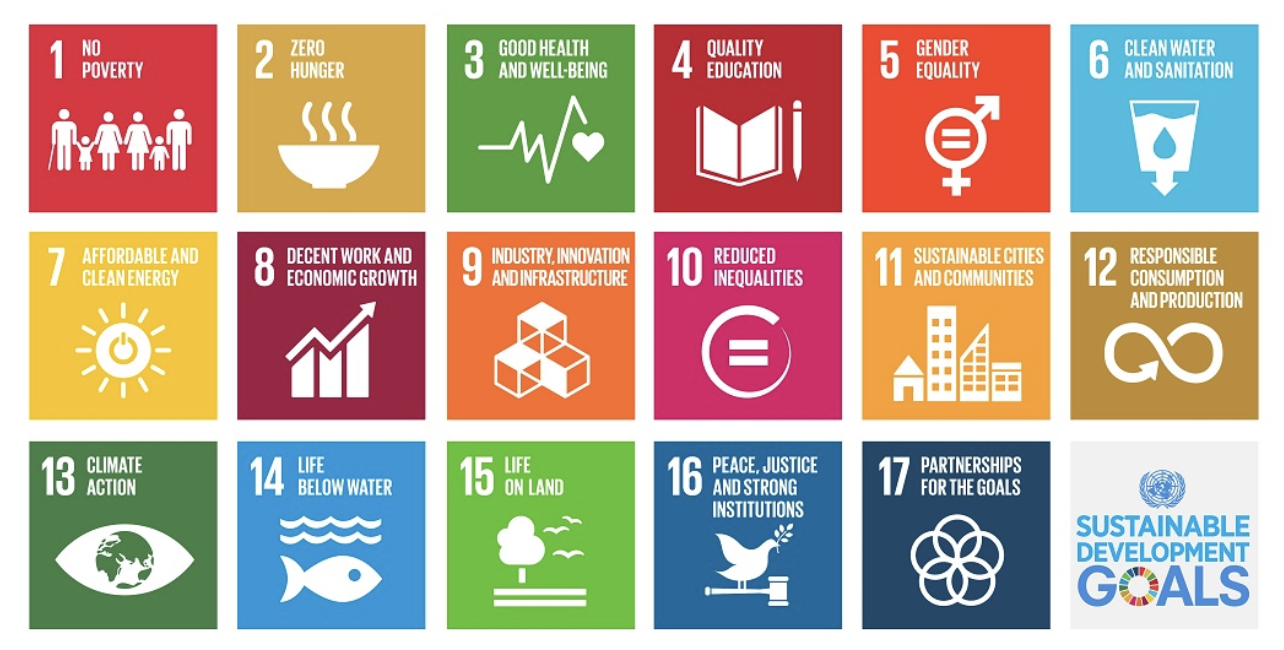
\includegraphics[width=0.8\linewidth]{media/SGD.png}
    \caption{17 Global Challenge for Government Transparency: The Sustainable Development Goals (SDG) 2030 Agenda }
    \label{fig:global_challenges}
\end{figure}

Gallstone disease is a common condition that may remain asymptomatic but can lead to complications such as acute cholecystitis, biliary obstruction, cholangitis, and pancreatitis \parencite{lammert2016gallstones,fujita2023guidelines}. Diagnosis generally relies on clinical assessment and abdominal ultrasonography. However, identifying high-risk individuals before complications occur may support earlier investigation and improve the efficient use of healthcare resources.

This project therefore develops a data-mining solution for the early prediction of gallstone disease using demographic, comorbidity, laboratory, and body-composition information. The Gallstone dataset contains records from 319 participants, including both patients with gallstones and control participants \parencite{esen2024early,uci2025gallstone}. Machine-learning models will be used to identify patterns associated with gallstone status and estimate individual disease risk.

The proposed solution is intended as a clinical decision-support tool rather than a replacement for medical diagnosis. By evaluating predictive performance, sensitivity, interpretability, and important risk factors, the project aims to demonstrate how data-driven healthcare can support preventive intervention, reduce avoidable complications, and improve resource allocation. In this way, the project contributes to a more proactive, efficient, and sustainable healthcare system aligned with the broader objectives of SDG 3.


% 2. BUSINESS AND SITUATION UNDERSTANDING
\section{Business and Situation Understanding}
\label{sec:business-understanding}
\subsection{Clinical background and motivation}

Gallstone disease (cholelithiasis) is a common hepatobiliary disorder in which solid deposits form within the gallbladder or biliary tract. Although many gallstones remain clinically silent, obstruction of the cystic or common bile duct can lead to biliary colic and complications such as acute cholecystitis, obstructive jaundice, cholangitis, and gallstone pancreatitis \cite{lammert2016gallstones,fujita2023guidelines}. A recent systematic review and meta-analysis estimated that approximately 6\% of the global population has gallstones, with prevalence varying substantially by sex and geographical region \cite{wang2024global}. The scale of the condition and the possibility of clinically important complications make the identification of individuals at increased risk a relevant preventive and diagnostic-support problem.

Gallstone formation is multifactorial rather than the result of a single abnormal measurement. Established or commonly reported associations include age, sex, obesity and body-fat distribution, metabolic abnormalities, dyslipidaemia, and diabetes \cite{lammert2016gallstones}. These relationships are relevant to the present dataset because its predictors combine demographic information, comorbidities, body-composition measurements, and routine laboratory markers. This creates an opportunity to investigate whether the joint pattern of routinely obtainable variables contains sufficient information to distinguish patients with and without gallstones.

In current clinical practice, abdominal ultrasonography remains a principal first-line imaging method for suspected gallstone disease, together with appropriate laboratory assessment \cite{easl2016guidelines,nice2014gallstone,fujita2023guidelines,gutt2020treatment}. Therefore, the purpose of the proposed machine learning system is \emph{not} to replace ultrasound or provide an autonomous diagnosis. Instead, the project treats prediction as a risk-stratification and decision-support problem: a model could estimate the probability of gallstone disease from non-imaging clinical information and thereby identify individuals who may warrant closer clinical assessment or confirmatory imaging.

This direction is supported by recent work applying machine learning to clinical and metabolic information. Salem et al.\ combined metabolomic and clinical predictors and demonstrated that nonlinear models can capture patterns associated with gallstone status \cite{salem2023ml}. More directly, Esen et al.\ introduced the dataset used in this project and reported that models based on bioimpedance and laboratory variables could distinguish gallstone cases from controls, with their strongest models reaching approximately 85\% accuracy and an area under the receiver-operating-characteristic curve (ROC--AUC) of about 0.85 \cite{esen2024early}. These results provide a useful benchmark, but they do not remove the need for careful validation, because the available sample is small and originates from a single clinical setting.

\subsection{Business and situation objectives}
\label{subsec:business-objectives}

The practical objective of this project is to develop and evaluate an interpretable early-risk prediction approach for gallstone disease using information that may already be available from routine clinical assessment, blood testing, and bioimpedance measurement. In a realistic healthcare workflow, the intended output would be a \emph{risk estimate} rather than a definitive diagnostic label. The model should help prioritise patients for further assessment while maintaining sufficient transparency for its predictions to be examined by a clinician.

Accordingly, the business/situation objectives are:

\begin{enumerate}
    \item Determine whether demographic, comorbidity, laboratory, and body-composition variables can provide useful early discrimination between patients with and without gallstones;
    \item Minimise clinically undesirable false-negative predictions, because a model that frequently classifies gallstone cases as low risk would have limited screening value;
    \item Identify the variables that contribute most strongly to predictions so that the resulting model remains interpretable and clinically reviewable; and
    \item Produce a reproducible proof-of-concept that can justify, but not substitute for, subsequent external clinical validation.
\end{enumerate}

For this iteration, business success is defined as evidence that the dataset can support a stable and interpretable risk-stratification model rather than evidence that the model is ready for clinical deployment. The analytical success criteria are therefore set as: (i) ROC--AUC of at least 0.80 under a validation procedure that keeps training and evaluation data separate; (ii) sensitivity/recall of at least 0.80 for the gallstone class at the selected decision threshold; (iii) performance superior to simple baselines such as majority-class prediction and standard logistic regression where possible; and (iv) reporting of calibration, confusion-matrix outcomes, and important predictors in addition to overall accuracy. These thresholds are project benchmarks chosen to make the data-mining goal measurable; they are not clinical guideline thresholds.

\subsection{Situation assessment}
\label{subsec:situation-assessment}

\subsubsection{Available resources and data}

The UCI Gallstone dataset originates from a prospective descriptive study conducted at the Internal Medicine Outpatient Clinic of Ankara VM Medical Park Hospital between June 2022 and June 2023 \cite{esen2024early,uci2025gallstone}. The source study initially considered 454 participants and excluded individuals who had previously undergone gallbladder surgery, leaving 319 participants for analysis: 161 with gallstones and 158 controls \cite{esen2024early}. The near-balanced outcome distribution is advantageous for a binary classification exercise because the model is not forced to learn from a severely under-represented positive class.

The dataset contains demographic variables, comorbidities, anthropometric measurements, bioimpedance measurements, hepatic-fat information, and routine laboratory results. Examples include age, sex, body mass index (BMI), diabetes, hyperlipidaemia, total body water, extracellular and intracellular water, body-fat and lean-mass measures, visceral fat measures, glucose, lipid markers, liver enzymes, creatinine, glomerular filtration rate, C-reactive protein (CRP), haemoglobin, and vitamin D \cite{esen2024early,uci2025gallstone}. The UCI repository describes the released data as having no missing values \cite{uci2025gallstone}; however, this must still be confirmed programmatically before modelling rather than assumed from documentation alone.

The dataset is computationally small and can be analysed on ordinary hardware. All development in this iteration will use Python, with reproducible scripts and notebooks used to record data validation, preprocessing, feature engineering, model fitting, and evaluation. The principal libraries are pandas and NumPy for data handling, scikit-learn for preprocessing, validation, and baseline models, and XGBoost and LightGBM for boosted-tree experiments.

\subsubsection{Requirements and assumptions}

Several requirements follow from the medical context. First, all predictor transformations must be fitted using training data only so that information from the evaluation set cannot leak into model development. Second, model performance must be reported with class-sensitive metrics---particularly sensitivity, specificity, precision, F1 score, ROC--AUC, and the confusion matrix---rather than accuracy alone. Third, model interpretation is required because a high-performing but opaque model would be difficult to justify as clinical decision support. Finally, the analysis should distinguish prediction from causal inference: an important feature may improve classification without being a causal determinant of gallstone formation.

A critical data-validation requirement is to verify the target encoding directly from the supplied dataset before analysis. The published study describes one numerical coding for gallstone presence, whereas the UCI repository documentation presents the class labels differently \cite{esen2024early,uci2025gallstone}. Similarly, repository metadata and the study description should be reconciled for the final number of observations. These discrepancies do not prevent modelling, but failure to resolve them could invert the target labels or create incorrect performance interpretation.

\subsubsection{Constraints, risks, and contingencies}

The principal constraint is sample size. With only approximately 319 participants and a relatively large number of candidate predictors, flexible models can overfit the training data. This risk will be reduced through stratified resampling, cross-validation, regularisation or restricted model complexity, and comparison with simpler baselines. Hyperparameter tuning and feature selection must occur inside the training/resampling process rather than on the full dataset.

A second constraint is external validity. The records come from a single hospital population in Ankara, and the observed relationships may not transfer directly to other countries, ethnic groups, age structures, or healthcare settings. Consequently, even strong internal validation results should be described as proof-of-concept evidence. External validation on an independent cohort would be required before clinical use.

A third risk concerns measurement availability. Some variables, particularly detailed bioimpedance measurements, may not be collected in every routine clinical setting. To address this, the project should compare a full-feature model with a reduced model based on more routinely available demographic and laboratory variables. If predictive performance remains similar, the reduced model may provide greater practical value.

Other risks include correlated body-composition variables, unstable feature importance, hidden coding errors, and optimistic results caused by repeated experimentation on the same test data. The contingency plan is to preserve a clear evaluation protocol, report uncertainty across resamples, investigate highly correlated variables, and avoid claiming that a small improvement in a single metric represents clinically meaningful superiority.

\subsection{Data-mining goals}
\label{subsec:data-mining-goals}

The data-mining task is a supervised binary-classification problem in which gallstone status is the target variable. The immediate technical goals are to:

\begin{enumerate}
    \item Audit variable types, ranges, coding, duplicates, and missing values;
    \item Explore relationships between gallstone status and demographic, metabolic, laboratory, and body-composition predictors;
    \item Establish interpretable baselines using logistic regression and a simple tree-based model;
    \item Compare a limited set of nonlinear classifiers such as random forest and gradient boosting using consistent resampling;
    \item Tune decision thresholds with particular attention to sensitivity and false-negative errors;
    \item Assess probability calibration in addition to discrimination;
    \item Evaluate model behaviour across clinically relevant subgroups, especially sex and age groups where sample size permits; and
    \item Use interpretable feature-attribution or model-specific importance methods to identify variables that consistently contribute to predictions.
\end{enumerate}

These goals align directly with the business objective: the model is useful only if it can identify higher-risk individuals with acceptable sensitivity, provide a meaningful probability estimate, and explain the factors contributing to that estimate. The strongest model will therefore not automatically be the model with the highest raw accuracy; model selection will consider discrimination, sensitivity, calibration, stability, and interpretability together.

\subsection{Project plan for the current iteration}
\label{subsec:project-plan}

Table~\ref{tab:iteration-plan} summarises the iteration running from 21 August to 21 September 2026. Development is organised around a common Python evaluation framework so that the baseline, data-centric, and model-centric strategies can be compared fairly using the same data partitions and metrics.

\begin{table}[htbp]
\centering
\caption{Iteration plan for Python development and evaluation, 21 August--21 September 2026.}
\label{tab:iteration-plan}
\begin{tabularx}{\textwidth}{p{2.7cm} X X}
\toprule
\textbf{Dates} & \textbf{Main activities} & \textbf{Expected output} \\
\midrule
21--24 August & Confirm the business objective and success criteria; audit target coding, variable types, missing values, duplicates, ranges, and provenance in Python. & Validated problem statement, data dictionary, and data-quality log. \\
25--28 August & Complete exploratory analysis and implement a leakage-safe Python pipeline with fixed stratified 70/15/15 partitions and repeated seeds; establish logistic-regression and tree baselines. & Reproducible baseline workflow, saved split membership, and benchmark metrics. \\
29 August--5 September & Apply the \emph{data-centric strategy}: correct data-quality issues, assess transformations and outliers, engineer clinically meaningful features, compare full and reduced feature sets, and perform feature selection within cross-validation. & Audited feature sets and evidence of whether data improvements increase validation performance and stability. \\
29 August--8 September & In parallel, apply the \emph{model-centric strategy}: compare logistic regression, random forest, Extra Trees, support-vector machine, XGBoost, LightGBM, and stacking; tune promising models without accessing the test set. & Tuned candidate models and a cross-validated comparison table. \\
9--13 September & Evaluate alternative validation strategies using repeated stratified holdout and leave-one-out cross-validation (LOOCV); assess threshold choice, calibration, sensitivity, specificity, ROC--AUC, F1, and log loss. & Robustness analysis showing the effect of evaluation strategy and decision threshold. \\
14--17 September & Conduct error analysis, subgroup checks, feature-importance analysis, and comparison of data-centric, model-centric, and combined strategies. & Error profiles, interpretation outputs, and a defensible preferred approach. \\
18--21 September & Re-run the selected workflow, verify reproducibility, consolidate results and limitations, and finalise the report and recommendations. & Reproducible Python artefacts and final iteration report. \\
\bottomrule
\end{tabularx}
\end{table}

\subsubsection{Development and data-mining plan}
The current iteration is scheduled from 21 August to 21 September 2026. All
development will be completed in Python. The work begins with a reproducible
baseline and then separates improvement activities into two complementary
strategies. The data-centric strategy improves the quality and representation
of the input data through validation, transformation, feature engineering,
feature selection, and reduced-feature experiments. The model-centric strategy
holds the prepared data and evaluation rules constant while comparing model
families, hyperparameters, ensembles, calibration, and classification
thresholds. A final combined strategy uses only improvements supported by
validation evidence.

Figure~\ref{fig:gantt-iteration} presents the project timeline. The same saved
data partitions and metrics will be used across strategies to ensure that any
observed improvement is attributable to the tested change rather than to a
different evaluation setup.

\begin{figure}[H]
\centering
\resizebox{\textwidth}{!}{%
\begin{ganttchart}[
    hgrid,
    vgrid,
    time slot format=isodate,
    title/.style={fill=gray!20},
    title label font=\bfseries\small,
    bar label font=\small,
    group label font=\bfseries\small,
    bar/.style={fill=blue!45},
    group/.style={fill=blue!70},
    milestone/.style={fill=red},
    x unit=0.36cm,
    y unit chart=0.55cm,
    y unit title=0.55cm
]{2026-08-21}{2026-09-21}

% Timeline
\gantttitle{August 2026}{11}
\gantttitle{September 2026}{21} \\
\gantttitlelist{21,23,...,29}{2}
\gantttitle{31}{1}
\gantttitlelist{1,3,...,19}{2}
\gantttitle{21}{1} \\

% Phase 1
\ganttgroup{Phase 1: Problem and Data Validation}
    {2026-08-21}{2026-08-24} \\

\ganttbar{Validate objective, target, variables, and provenance}
    {2026-08-21}{2026-08-24} \\

% Phase 2
\ganttgroup{Phase 2: Python Baseline and Evaluation Design}
    {2026-08-25}{2026-08-28} \\

\ganttbar{EDA, saved splits, pipelines, and baselines}
    {2026-08-25}{2026-08-28} \\

% Phase 3
\ganttgroup{Phase 3: Parallel Strategy Development}
    {2026-08-29}{2026-09-08} \\

\ganttbar[bar/.append style={fill=teal!55}]{Data-centric: quality, features, and selection}
    {2026-08-29}{2026-09-05} \\

\ganttbar[bar/.append style={fill=orange!65}]{Model-centric: compare, tune, and stack}
    {2026-08-29}{2026-09-08} \\

% Phase 4
\ganttgroup{Phase 4: Strategy Evaluation}
    {2026-09-09}{2026-09-13} \\

\ganttbar{Repeated holdout, LOOCV, metrics, and thresholds}
    {2026-09-09}{2026-09-13} \\

% Phase 5
\ganttgroup{Phase 5: Error Analysis and Strategy Selection}
    {2026-09-14}{2026-09-17} \\

\ganttbar{Errors, subgroups, interpretation, and comparison}
    {2026-09-14}{2026-09-17} \\

% Phase 6
\ganttgroup{Phase 6: Reproducibility and Reporting}
    {2026-09-18}{2026-09-21} \\

\ganttbar{Re-run workflow and finalise report}
    {2026-09-18}{2026-09-21} \\

\ganttmilestone{Current iteration completed}
    {2026-09-21}

\end{ganttchart}%
}
\caption{Python development and evaluation plan for the current gallstone
prediction iteration, 21 August--21 September 2026.}
\label{fig:gantt-iteration}
\end{figure}

The baseline strategy provides the reference result against which subsequent
changes are assessed. In the data-centric stage, models are deliberately kept
stable while changes to data quality, transformations, engineered variables,
and feature subsets are evaluated. In the model-centric stage, the selected
data representation is held stable while algorithms and hyperparameters are
varied. Preprocessing and feature selection remain inside each resampling fold
to prevent leakage. Repeated holdout evaluation measures variation across
partitions, while LOOCV provides a complementary assessment that uses nearly
all observations for training in each fold. The preferred approach will be
selected using sensitivity, specificity, ROC--AUC, F1, calibration, stability,
interpretability, and implementation complexity rather than accuracy alone.

Figure~\ref{fig:python-project-pipeline} clarifies the experimental pipeline.
The untouched test partition is used only after the data-centric and
model-centric choices have been made from training and validation evidence.

\begin{figure}[H]
\centering
\resizebox{\textwidth}{!}{%
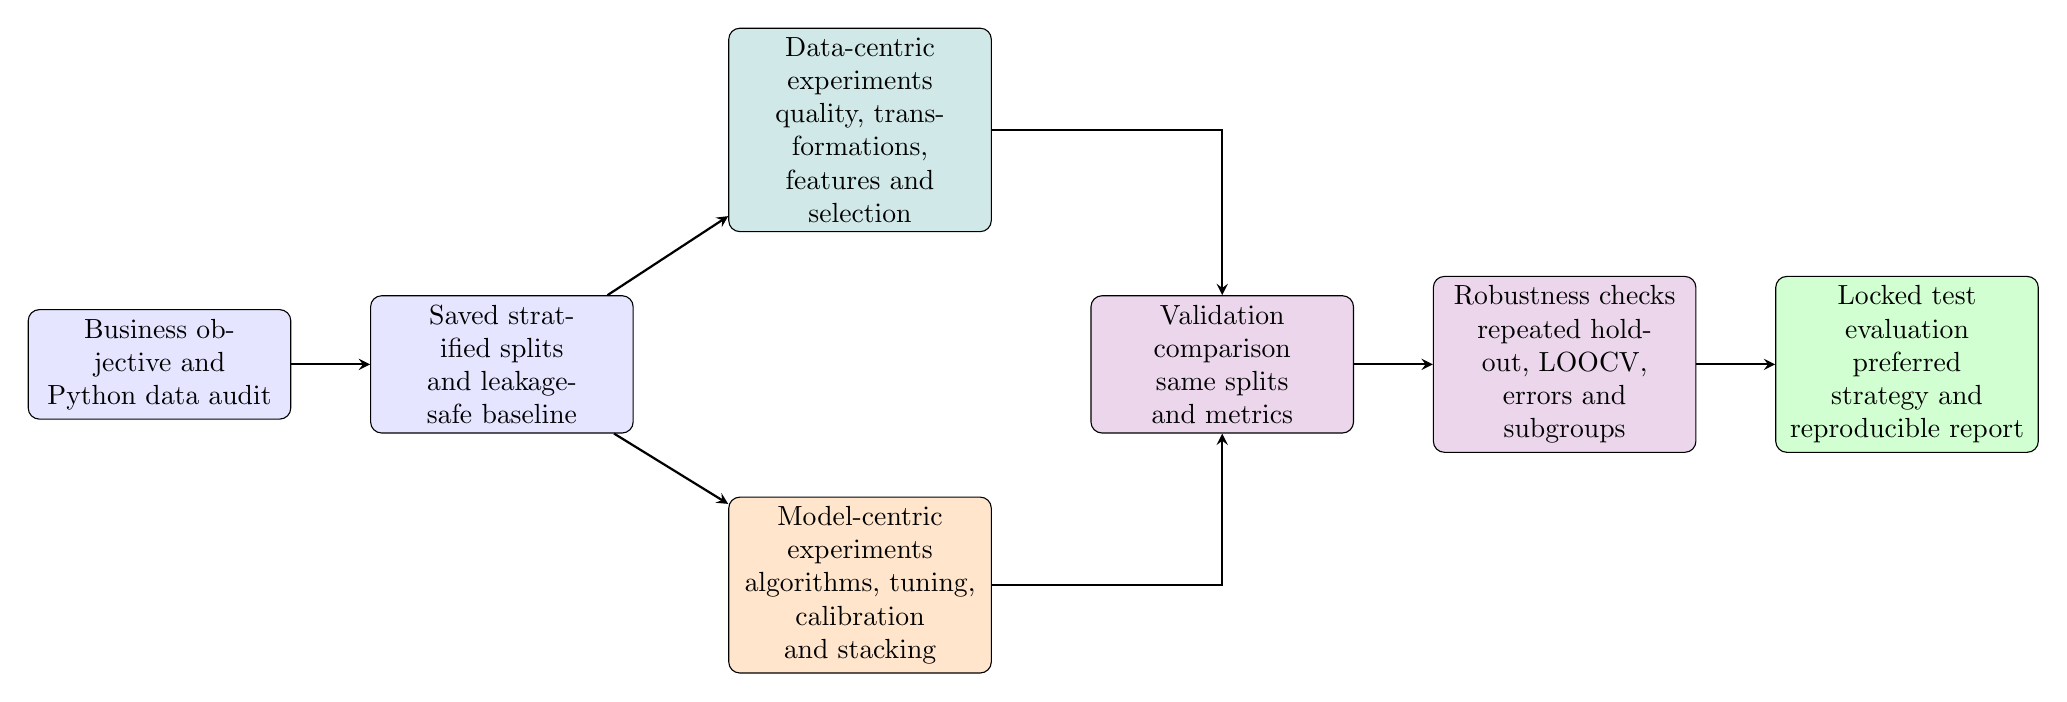
\begin{tikzpicture}[
    node distance=7mm and 10mm,
    stage/.style={draw, rounded corners, align=center, minimum height=9mm,
                  text width=3.1cm, fill=blue!10},
    data/.style={stage, fill=teal!18},
    model/.style={stage, fill=orange!20},
    decision/.style={stage, fill=violet!16},
    output/.style={stage, fill=green!18},
    arrow/.style={->, thick, >=stealth}
]
\node[stage] (audit) {Business objective and\\Python data audit};
\node[stage, right=of audit] (split) {Saved stratified splits\\and leakage-safe baseline};
\node[data, above right=8mm and 12mm of split] (datacentric)
    {Data-centric experiments\\quality, transformations,\\features and selection};
\node[model, below right=8mm and 12mm of split] (modelcentric)
    {Model-centric experiments\\algorithms, tuning,\\calibration and stacking};
\node[decision, right=58mm of split] (compare)
    {Validation comparison\\same splits and metrics};
\node[decision, right=of compare] (robust)
    {Robustness checks\\repeated holdout, LOOCV,\\errors and subgroups};
\node[output, right=of robust] (final)
    {Locked test evaluation\\preferred strategy and\\reproducible report};

\draw[arrow] (audit) -- (split);
\draw[arrow] (split) -- (datacentric);
\draw[arrow] (split) -- (modelcentric);
\draw[arrow] (datacentric.east) -| (compare.north);
\draw[arrow] (modelcentric.east) -| (compare.south);
\draw[arrow] (compare) -- (robust);
\draw[arrow] (robust) -- (final);
\end{tikzpicture}
}
\caption{Python project pipeline for comparing data-centric, model-centric,
and combined gallstone-prediction strategies.}
\label{fig:python-project-pipeline}
\end{figure}

\subsubsection{Report writing plan}
\label{subsec:report-writing-plan}

Report writing will be carried out progressively throughout the current
iteration rather than being postponed until the modelling work is complete.
Early sections describing the problem, dataset, and methodology will be
drafted while the corresponding analytical tasks are being completed.
Results, discussion, limitations, and recommendations will then be added as
model outputs become available. This approach allows the report to be updated continuously and reduces the risk of documentation being disconnected from the implemented analysis.

Figure~\ref{fig:gantt-report-writing} presents the report-writing schedule for
21 August--21 September 2026.

\begin{figure}[H]
\centering
\resizebox{\textwidth}{!}{%
\begin{ganttchart}[
    hgrid,
    vgrid,
    time slot format=isodate,
    title/.style={fill=gray!20},
    title label font=\bfseries\small,
    bar label font=\small,
    group label font=\bfseries\small,
    bar/.style={fill=green!45},
    group/.style={fill=green!70},
    milestone/.style={fill=red},
    x unit=0.36cm,
    y unit chart=0.55cm,
    y unit title=0.55cm
]{2026-08-21}{2026-09-21}

% Timeline
\gantttitle{August 2026}{11}
\gantttitle{September 2026}{21} \\
\gantttitlelist{21,23,...,29}{2}
\gantttitle{31}{1}
\gantttitlelist{1,3,...,19}{2}
\gantttitle{21}{1} \\

% Planning
\ganttgroup{Report Planning and Structure}
    {2026-08-21}{2026-08-23} \\

\ganttbar{Define report structure and section outline}
    {2026-08-21}{2026-08-22} \\

\ganttbar{Organise references and supporting materials}
    {2026-08-22}{2026-08-23} \\

% Introduction
\ganttgroup{Introduction and Problem Definition}
    {2026-08-24}{2026-08-28} \\

\ganttbar{Draft background and motivation}
    {2026-08-24}{2026-08-25} \\

\ganttbar{Write problem statement and objectives}
    {2026-08-26}{2026-08-27} \\

\ganttbar{Write project scope and success criteria}
    {2026-08-28}{2026-08-28} \\

% Data and Methodology
\ganttgroup{Data and Methodology}
    {2026-08-29}{2026-09-05} \\

\ganttbar{Document dataset and variables}
    {2026-08-29}{2026-08-30} \\

\ganttbar{Write data quality and EDA section}
    {2026-08-31}{2026-09-01} \\

\ganttbar{Document preprocessing and evaluation design}
    {2026-09-02}{2026-09-03} \\

\ganttbar{Describe baseline and candidate models}
    {2026-09-04}{2026-09-05} \\

% Results
\ganttgroup{Results}
    {2026-09-06}{2026-09-13} \\

\ganttbar{Prepare model performance tables}
    {2026-09-06}{2026-09-08} \\

\ganttbar{Prepare figures and visualisations}
    {2026-09-09}{2026-09-10} \\

\ganttbar{Write model comparison results}
    {2026-09-11}{2026-09-12} \\

\ganttbar{Write threshold and calibration results}
    {2026-09-13}{2026-09-13} \\

% Discussion
\ganttgroup{Discussion and Interpretation}
    {2026-09-14}{2026-09-17} \\

\ganttbar{Interpret predictive performance}
    {2026-09-14}{2026-09-14} \\

\ganttbar{Discuss feature importance and clinical relevance}
    {2026-09-15}{2026-09-16} \\

\ganttbar{Document limitations and risks}
    {2026-09-17}{2026-09-17} \\

% Finalisation
\ganttgroup{Finalisation}
    {2026-09-18}{2026-09-21} \\

\ganttbar{Write conclusion and recommendations}
    {2026-09-18}{2026-09-18} \\

\ganttbar{Review consistency, citations, tables, and figures}
    {2026-09-19}{2026-09-20} \\

\ganttbar{Proofread and finalise report}
    {2026-09-21}{2026-09-21} \\

\ganttmilestone{Final report completed}
    {2026-09-21}

\end{ganttchart}%
}
\caption{Day-to-day report-writing plan for the gallstone prediction project,
21 August--21 September 2026.}
\label{fig:gantt-report-writing}
\end{figure}

The completion criterion for this iteration is therefore a transparent comparison of feasible predictive models and a defensible conclusion about whether this dataset supports early gallstone-risk stratification. Clinical deployment, treatment decisions, and replacement of diagnostic imaging are explicitly outside the scope of the present iteration.


% 3. DATA UNDERSTANDING
\section{Data understanding}
\label{sec:data-understanding}
\subsection{Initial Data Collection}
\label{subsec:initial-data-collection}

The dataset used in this project was obtained from the UCI Machine Learning Repository and originates from the clinical study conducted by \textcite{esen2024early}. The original data were collected prospectively from patients attending the Internal Medicine Outpatient Clinic of Ankara VM Medical Park Hospital, Turkey, between June 2022 and June 2023 \parencite{esen2024early,uci2025gallstone}.

The original study initially collected information from 454 participants. Records from individuals who had previously undergone gallbladder surgery were excluded, resulting in a final published dataset of 319 participants. Among these, 161 participants were diagnosed with gallstone disease and 158 formed the control group \parencite{esen2024early}. Data collection included demographic and clinical characteristics, comorbidities, laboratory test results, and body-composition measurements obtained through bioimpedance analysis. The resulting dataset contains 38 predictive attributes relating to factors such as age, BMI, diabetes, lipid profiles, liver-function markers, glucose levels, body water, muscle mass, and body-fat distribution/

No additional primary data were collected for the current project; therefore, this analysis represents secondary use of the published clinical dataset. The UCI repository reports no missing values. However, an issue identified during initial data collection and validation is an inconsistency in the published metadata: the repository description reports 319 participants, while one metadata field lists 320 instances. Consequently, the downloaded dataset's row count and target coding will be independently verified before further analysis.

The dataset was downloaded in tabular form and will be retained in its original form as a raw-data copy before any cleaning or transformation is performed.

\subsection{Data Description}
\label{subsec:data-description}

The dataset contains one binary target variable, \textit{Gallstone Status}, and 38 predictor variables covering demographic characteristics, comorbidities, anthropometric measurements, body-composition indicators, and laboratory measurements. The predictors include both categorical and numerical variables, allowing the project to investigate multiple clinical and physiological factors that may be associated with gallstone disease.

According to the dataset documentation, no missing values are reported. However, the variable types, class coding, ranges, and missing-value patterns will be independently verified during the data-quality assessment before modelling. In particular, categorical variables stored numerically will be converted to appropriate factor or categorical representations to prevent their codes from being interpreted as continuous quantities.

Table~\ref{tab:data-dictionary} summarises the variables contained in the dataset.

\begin{longtable}{
    p{4.0cm}
    p{1.3cm}
    p{1.6cm}
    p{1.4cm}
    p{5.0cm}
    p{1.0cm}
    p{1.2cm}
}
\caption{Data dictionary for the Gallstone dataset.}
\label{tab:data-dictionary} \\

\toprule
\textbf{Variable} &
\textbf{Role} &
\textbf{Type} &
\textbf{Demo.} &
\textbf{Description} &
\textbf{Units} &
\textbf{Missing} \\
\midrule
\endfirsthead

\multicolumn{7}{c}%
{{\tablename\ \thetable{} -- continued from previous page}} \\

\toprule
\textbf{Variable} &
\textbf{Role} &
\textbf{Type} &
\textbf{Demo.} &
\textbf{Description} &
\textbf{Units} &
\textbf{Missing} \\
\midrule
\endhead

\midrule
\multicolumn{7}{r}{{Continued on next page}} \\
\endfoot

\bottomrule
\endlastfoot

Gallstone Status
& Target & Binary & -- 
& Presence or absence of gallstones 
& -- & No \\

Age
& Feature & Integer & Age
& Age of the participant
& years & No \\

Gender
& Feature & Categorical & Gender
& Gender of the participant
& -- & No \\

Comorbidity
& Feature & Categorical & --
& Number of concomitant medical conditions
& -- & No \\

Coronary Artery Disease (CAD)
& Feature & Binary & --
& Presence of coronary artery disease
& -- & No \\

Hypothyroidism
& Feature & Binary & --
& Presence of an underactive thyroid gland
& -- & No \\

Hyperlipidemia
& Feature & Binary & --
& Presence of elevated blood lipid levels
& -- & No \\

Diabetes Mellitus (DM)
& Feature & Binary & --
& Presence of diabetes mellitus
& -- & No \\

Height
& Feature & Integer & --
& Height of the participant
& -- & No \\

Weight
& Feature & Continuous & --
& Body weight of the participant
& -- & No \\

Body Mass Index (BMI)
& Feature & Continuous & --
& Weight relative to height
& -- & No \\

Total Body Water (TBW)
& Feature & Continuous & --
& Total amount of water in the body
& -- & No \\

Extracellular Water (ECW)
& Feature & Continuous & --
& Amount of water outside body cells
& -- & No \\

Intracellular Water (ICW)
& Feature & Continuous & --
& Amount of water contained within body cells
& -- & No \\

Extracellular Fluid/Total Body Water (ECF/TBW)
& Feature & Continuous & --
& Ratio of extracellular fluid to total body water
& -- & No \\

Total Body Fat Ratio (TBFR)
& Feature & Continuous & --
& Proportion of total body mass consisting of fat
& \% & No \\

Lean Mass (LM)
& Feature & Continuous & --
& Proportion of lean body mass
& \% & No \\

Body Protein Content (Protein)
& Feature & Continuous & --
& Estimated proportion of body protein
& \% & No \\

Visceral Fat Rating (VFR)
& Feature & Integer & --
& Rating of visceral fat surrounding internal organs
& -- & No \\

Bone Mass (BM)
& Feature & Continuous & --
& Estimated bone mass
& -- & No \\

Muscle Mass (MM)
& Feature & Continuous & --
& Estimated amount of muscle mass
& -- & No \\

Obesity
& Feature & Continuous & --
& Estimated degree of excess adiposity
& \% & No \\

Total Fat Content (TFC)
& Feature & Continuous & --
& Estimated total amount of body fat
& -- & No \\

Visceral Fat Area (VFA)
& Feature & Continuous & --
& Estimated area of visceral adipose tissue
& -- & No \\

Visceral Muscle Area (VMA)
& Feature & Continuous & --
& Estimated visceral muscle measurement
& kg & No \\

Hepatic Fat Accumulation (HFA)
& Feature & Categorical & --
& Degree of fat accumulation in the liver
& -- & No \\

Glucose
& Feature & Continuous & --
& Blood glucose level
& -- & No \\

Total Cholesterol (TC)
& Feature & Continuous & --
& Total blood cholesterol level
& -- & No \\

Low Density Lipoprotein (LDL)
& Feature & Continuous & --
& Low-density lipoprotein cholesterol level
& -- & No \\

High Density Lipoprotein (HDL)
& Feature & Continuous & --
& High-density lipoprotein cholesterol level
& -- & No \\

Triglyceride
& Feature & Continuous & --
& Triglyceride concentration in the blood
& -- & No \\

Aspartate Aminotransferase (AST)
& Feature & Continuous & --
& Liver enzyme measurement
& -- & No \\

Alanine Aminotransferase (ALT)
& Feature & Continuous & --
& Liver enzyme measurement
& -- & No \\

Alkaline Phosphatase (ALP)
& Feature & Continuous & --
& Enzyme associated primarily with liver and bone
& -- & No \\

Creatinine
& Feature & Continuous & --
& Indicator associated with kidney function
& -- & No \\

Glomerular Filtration Rate (GFR)
& Feature & Continuous & --
& Estimated kidney filtration rate
& -- & No \\

C-Reactive Protein (CRP)
& Feature & Continuous & --
& Marker associated with systemic inflammation
& -- & No \\

Hemoglobin (HGB)
& Feature & Continuous & --
& Concentration of oxygen-carrying haemoglobin
& -- & No \\

Vitamin D
& Feature & Continuous & --
& Blood vitamin D level
& -- & No \\

\end{longtable}

\subsubsection{Categorical Variable Coding}
\label{subsubsec:categorical-coding}

Several categorical variables are represented by integer codes in the raw dataset. These values represent categories rather than continuous numerical quantities and therefore require appropriate treatment during preprocessing. The documented class labels are:

\begin{itemize}
    \item \textbf{Gallstone Status:}
    0 = gallstones present; 
    1 = gallstones absent.

    \item \textbf{Gender:}
    0 = male; 
    1 = female.

    \item \textbf{Comorbidity:}
    0 = no comorbidities;
    1 = one comorbid condition;
    2 = two comorbid conditions;
    3 = three or more comorbid conditions.

    \item \textbf{Coronary Artery Disease:}
    0 = no;
    1 = yes.

    \item \textbf{Hypothyroidism:}
    0 = no;
    1 = yes.

    \item \textbf{Hyperlipidemia:}
    0 = no;
    1 = yes.

    \item \textbf{Diabetes Mellitus:}
    0 = no;
    1 = yes.

    \item \textbf{Hepatic Fat Accumulation (HFA):}
    0 = no fat accumulation;
    1 = Grade 1 (mild);
    2 = Grade 2 (moderate);
    3 = Grade 3 (severe);
    4 = Grade 4 (very severe).
\end{itemize}

Although these categories are encoded numerically, they do not all have the same statistical interpretation. Binary variables such as diabetes and coronary artery disease can be represented as indicator variables, whereas \textit{Comorbidity} and \textit{Hepatic Fat Accumulation} are ordinal variables because their categories represent increasing levels of severity or burden. Their treatment during modelling will therefore be determined explicitly during the data-preparation stage.

\subsection{Data exploration}
\label{subsec:data-exploration}
Exploratory data analysis (EDA) was conducted on the raw dataset before any transformation or model training. The purpose was to understand the distribution of the target variable, examine the characteristics of the predictors, identify potential outliers or skewed variables, and investigate relationships that may influence subsequent data preparation and modelling.

\subsubsection{Target Variable Distribution} Figure~\ref{fig:target-distribution} shows the distribution of the target variable, \textit{Gallstone Status}. Based on the documented class encoding, 0 represents the presence of gallstones and 1 represents the absence of gallstones. 

\begin{figure}[H] 
    \centering 
    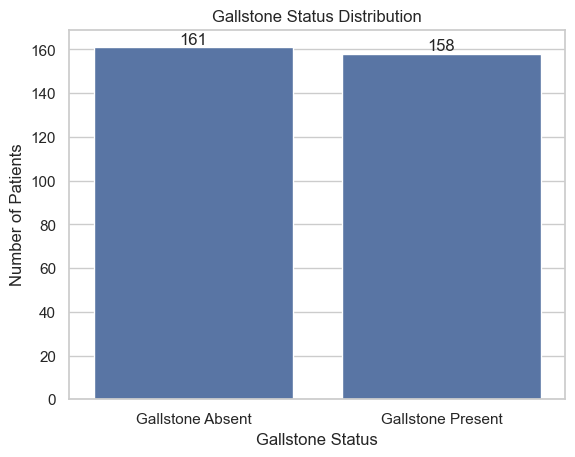
\includegraphics[width=0.8\textwidth]{media/binary_target_distirbution.png} 
    \caption{Distribution of Gallstone Status in the raw dataset.} 
    \label{fig:target-distribution} 
\end{figure} 

The dataset contains 161 participants with gallstones and 158 participants without gallstones. The two classes therefore account for approximately 50.5\% and 49.5\% of the observations, respectively. This indicates that the classification problem is almost perfectly balanced. This is an important characteristic for the subsequent modelling stage. Severe class imbalance is unlikely to be a major source of bias, and resampling techniques such as oversampling or undersampling are not immediately required. Nevertheless, stratified data partitioning will be used when dividing the observations into training and testing sets to preserve the approximately equal class proportions. Model evaluation will also consider sensitivity, specificity, F1-score and ROC-AUC rather than accuracy alone.

\subsubsection{Distribution of Continuous Features}
\label{sec:cont_distribution}

\begin{figure}[H]
    \centering
    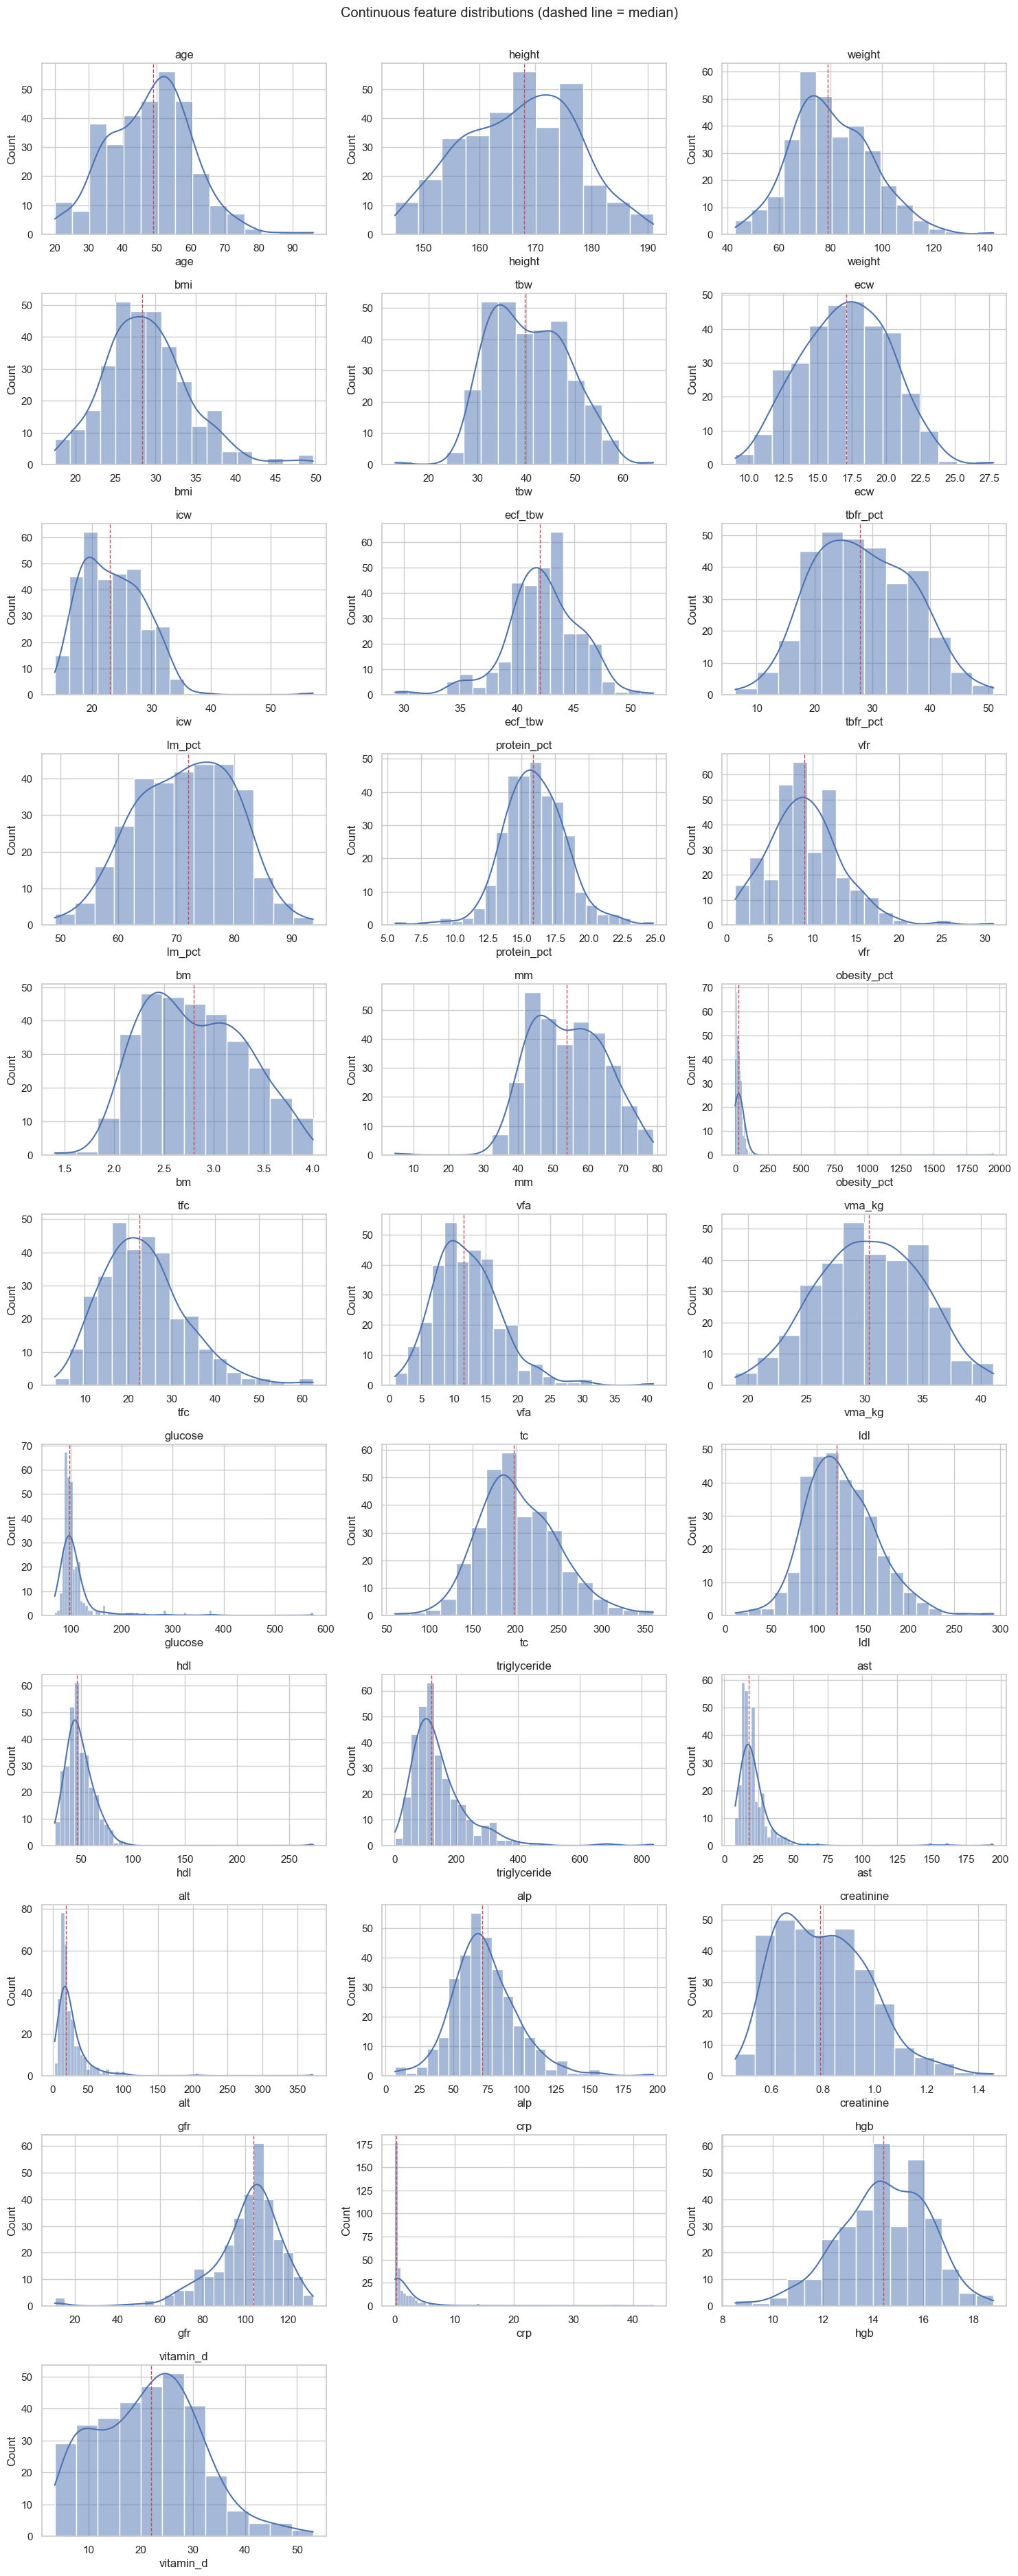
\includegraphics[
        width=\linewidth,
        height=0.75\textheight
    ]{media/Continous_Distribution.png}
    \caption{Distribution of continuous variables in the raw Gallstone dataset.
    The dashed vertical line represents the median.}
    \label{fig:cont-dis}
\end{figure}

Figure~\ref{fig:cont-dis} presents the distributions of the continuous variables before any transformation or outlier treatment. The plots show considerable variation in distributional shape across the clinical and body-composition measurements.

Several variables, including age, height, BMI, extracellular water (ECW), lean mass, creatinine, haemoglobin, and visceral muscle area, display relatively smooth and approximately unimodal distributions. In contrast, variables such as glucose, triglyceride, AST, ALT, CRP, visceral fat rating (VFR), visceral fat area (VFA), and total fat content (TFC) show noticeable right-skewness, with most observations concentrated at lower values and a small number of substantially larger measurements.

The distributions also reveal several extreme observations, particularly in metabolic and laboratory variables. These values require further assessment during the data-quality stage to determine whether they represent valid clinical measurements or potential data errors. They will not be removed automatically, as unusual values may contain clinically meaningful information relevant to gallstone risk.

Overall, this exploration indicates that the predictors differ substantially in both scale and distribution. Consequently, standardisation and possible transformations of strongly skewed variables will be considered during data preparation, depending on the modelling technique used. The next stage of the analysis compares these predictors with \textit{Gallstone Status} to identify variables that may provide useful discriminatory information for the classification models.

\subsubsection{Distribution of categorical features and Association with Gallstone Status}
\label{subsubsec:categorical-distribution}

The categorical predictors were examined by comparing both the class counts and
the proportion of participants with gallstones within each category. This
provides an initial indication of whether particular categorical variables may
contain useful discriminatory information for the prediction task.

\begin{figure}[H]
    \centering
    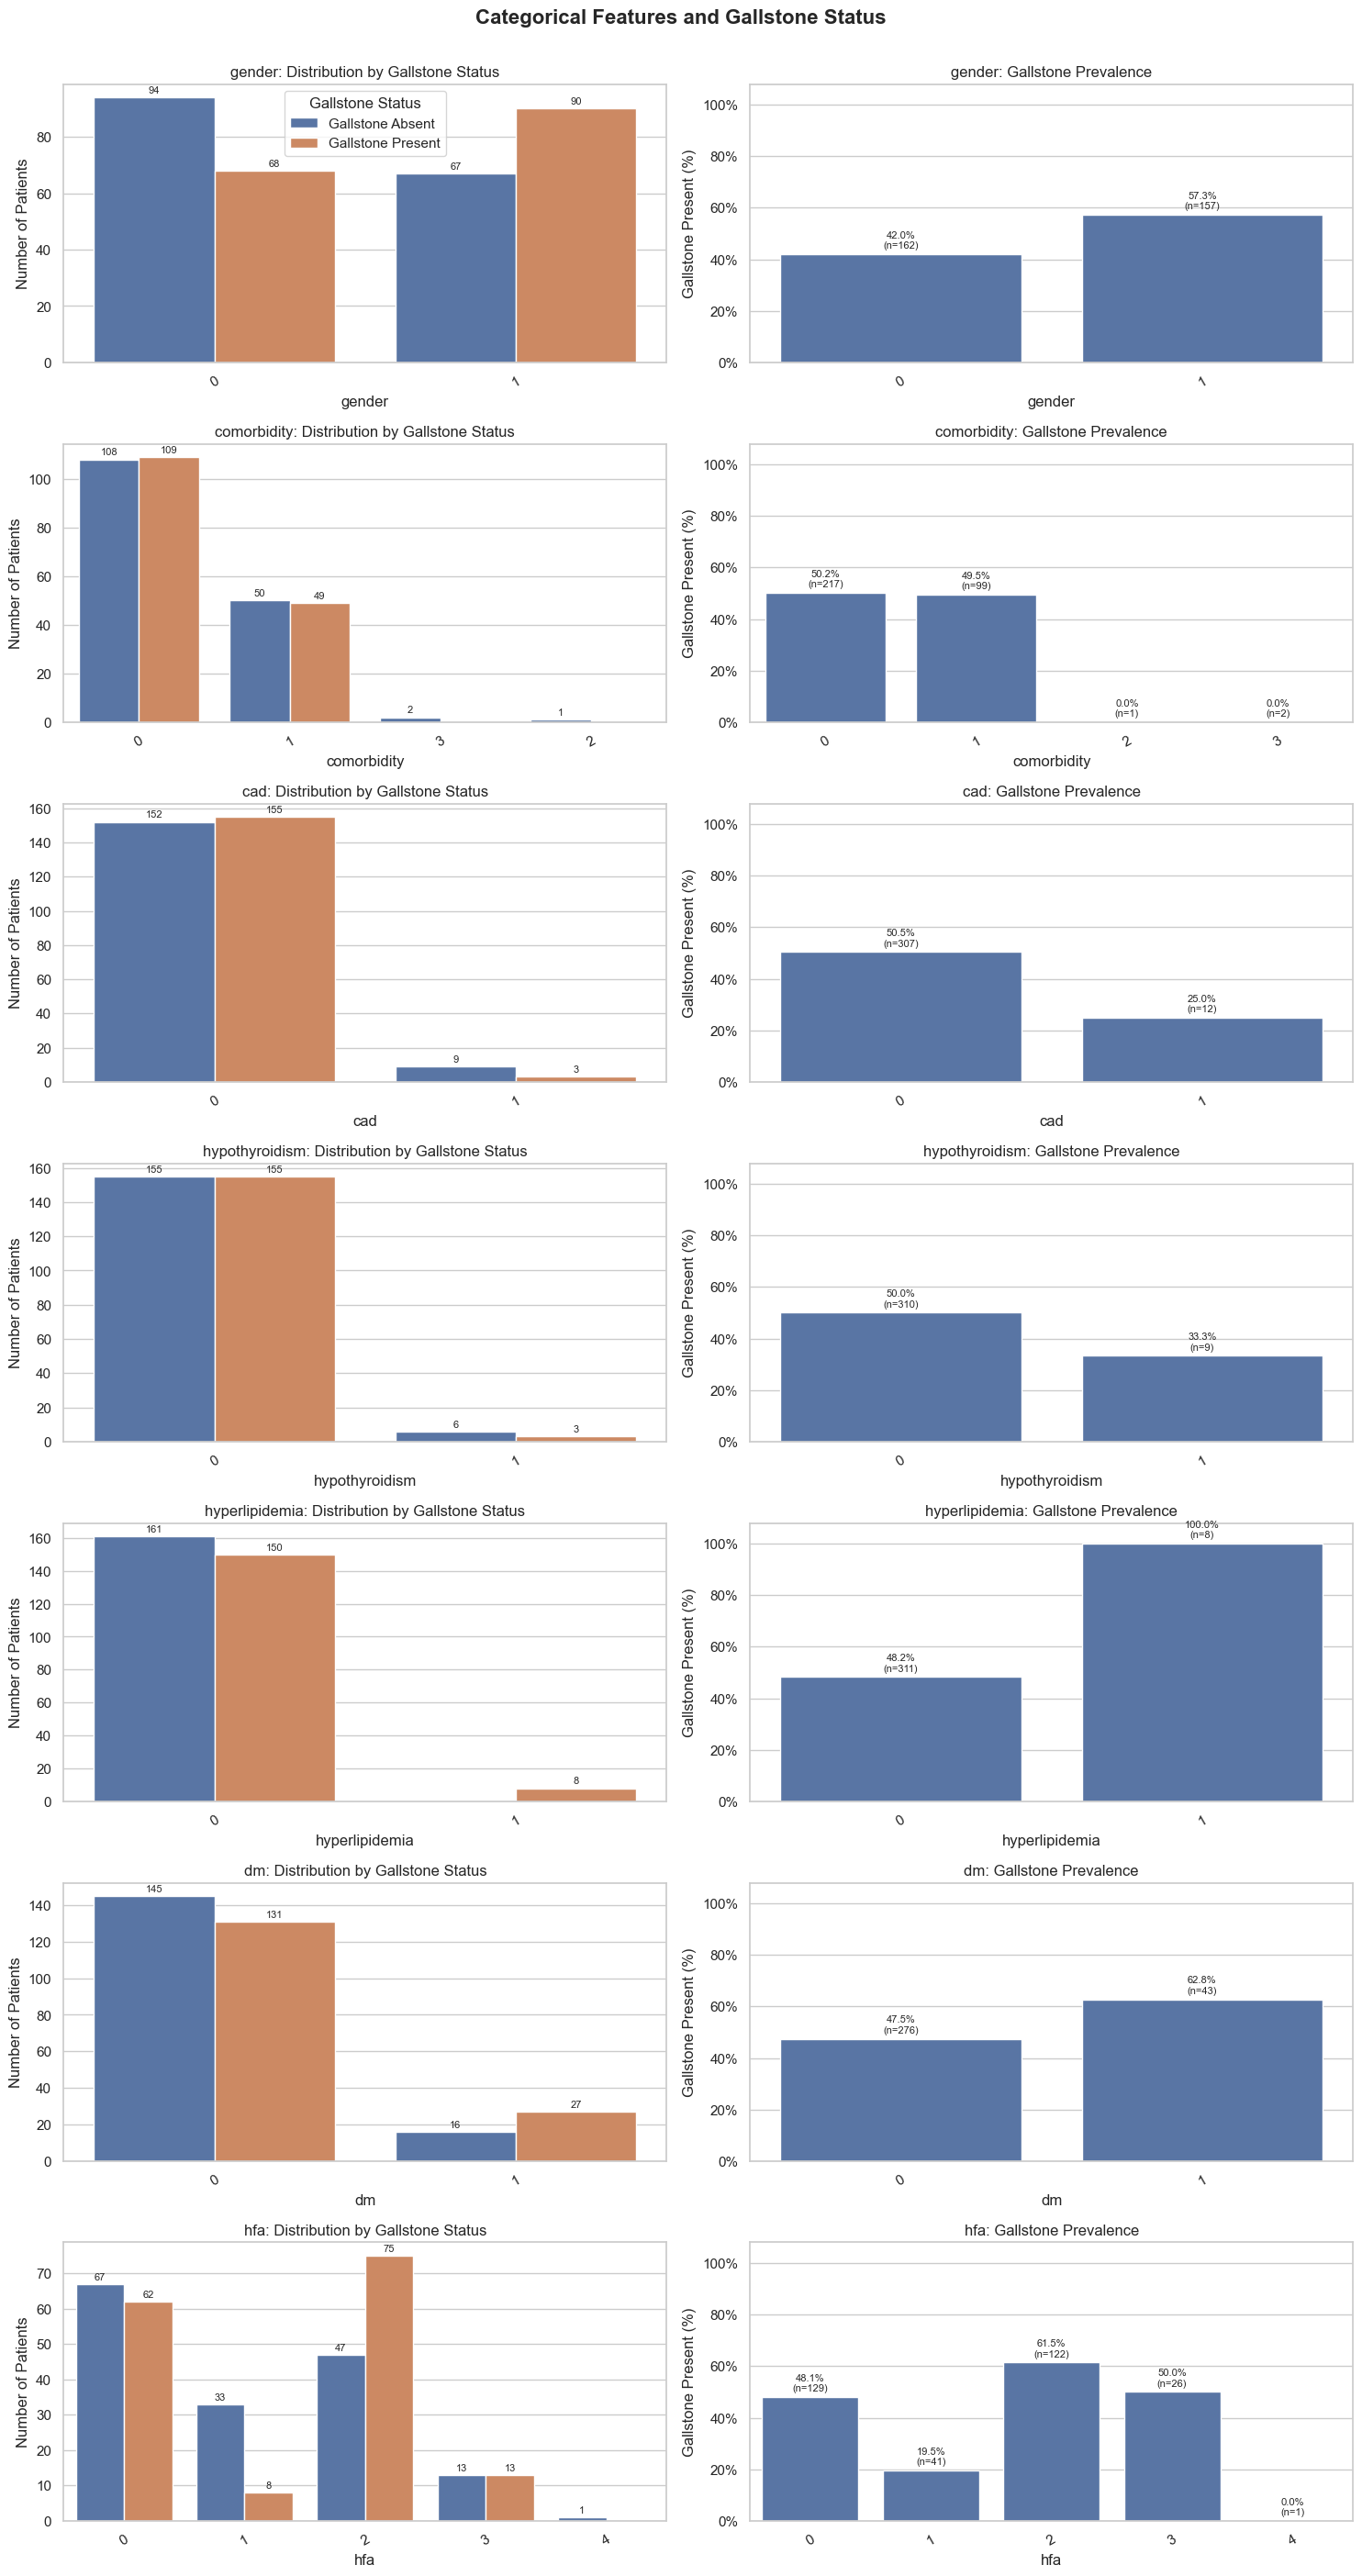
\includegraphics[
        width=0.7\linewidth,
        keepaspectratio
    ]{media/category_distribution.png}
    \caption{Distribution of categorical predictors by Gallstone Status and the
    corresponding gallstone prevalence within each category.}
    \label{fig:categorical-distribution}
\end{figure}

Figure~\ref{fig:categorical-distribution} suggests that the predictive signal
varies considerably across the categorical variables. Gender shows a moderate
difference between categories: the gallstone prevalence is approximately
42.0\% for category 0 and 57.3\% for category 1, indicating that gender may
provide some discriminatory information.

Diabetes mellitus (\texttt{dm}) also shows a potentially useful difference.
Gallstone prevalence is approximately 47.5\% among participants in category 0
compared with 62.8\% in category 1. A similar pattern is visible for
\texttt{hfa}, where prevalence varies across categories, most notably between
category 1 (19.5\%) and category 2 (61.5\%). This suggests that these variables
may contribute information useful for separating the two outcome classes.

In contrast, \texttt{comorbidity} shows little separation in the two major
categories, with gallstone prevalence close to 50\% in both. This indicates
limited univariate discriminatory value for this variable. \texttt{cad} and
\texttt{hypothyroidism} also show lower prevalence among category 1 than
category 0, although the number of observations in their positive categories is
small.

The strongest apparent difference is observed for \texttt{hyperlipidemia},
where all eight participants in category 1 have gallstones. However, this result
should be interpreted cautiously because the category contains very few
observations. Similar caution is required for rare levels of
\texttt{comorbidity} and \texttt{hfa}, where prevalence estimates are based on
only one or two participants and are therefore highly unstable.

Overall, the categorical EDA provides evidence of some class-related signal,
particularly for gender, diabetes mellitus, and selected HFA categories.
However, no single categorical predictor provides a sufficiently strong or
stable separation between participants with and without gallstones. The results
therefore support retaining these variables for multivariable modelling, where
their combined effects and interactions with continuous clinical and
body-composition measurements can be evaluated.


\subsubsection{Correlation Analysis}
\label{subsubsec:correlation}

Figure~\ref{fig:spearman-correlation} presents the Spearman correlationmatrix for the dataset. Spearman correlation was selected because several
continuous variables are skewed and contain extreme observations.

\begin{figure}[H]
    \centering
    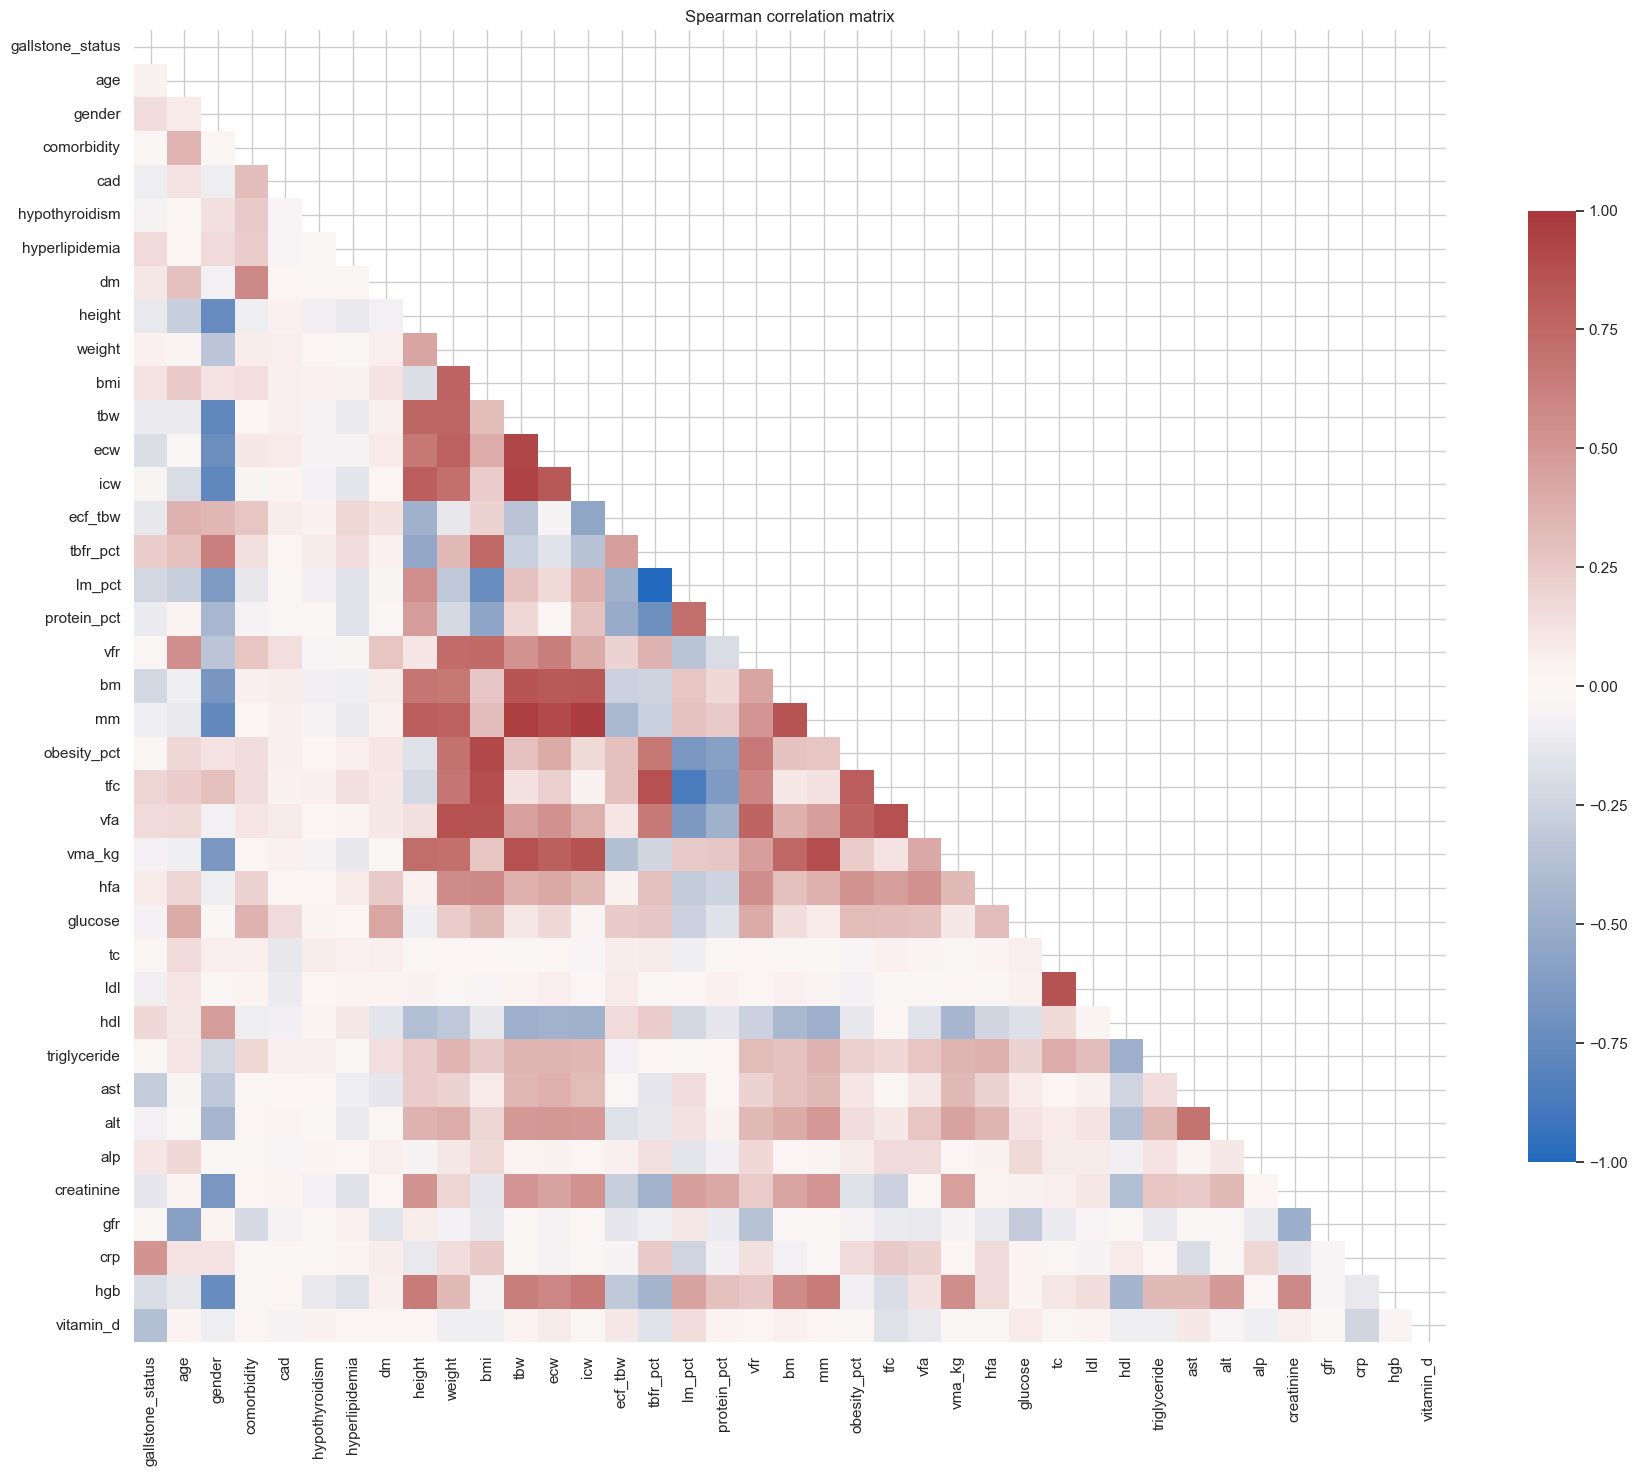
\includegraphics[width=0.75\textwidth]{media/correlation.png}
    \caption{Spearman correlation matrix for the Gallstone dataset visualization.}
    \label{fig:spearman-correlation}
\end{figure}

The matrix shows several groups of strongly related predictors. In particular, body-composition variables such as weight, BMI, TBW, ECW, ICW, muscle mass, body-fat measures, and visceral-fat measures show substantial correlation. Laboratory variables also contain related groups, including
TC-LDL, AST-ALT, and the inverse relationship between creatinine and GFR. These patterns indicate potential redundancy and multicollinearity among some predictors.

In contrast, individual correlations with \textit{Gallstone Status} are generally weaker. This suggests that gallstone status is unlikely to be explained by a single predictor and supports the use of multivariable classification models that combine demographic, body-composition, and
laboratory information.

These findings will guide the data-preparation stage. Highly correlated variables will be reviewed during feature selection, particularly for logistic regression, while tree-based models will also be considered because they are less sensitive to multicollinearity.


\subsubsection{Structure Among Body-Composition Variables} 

Some body-composition variables, including total body water (TBW), bone mass (BM), and muscle mass (MM), appear to have broader or mildly multi-peaked distributions. This may indicate underlying differences between participant subgroups, for example differences in sex, body size, or body composition. At this stage, however, the univariate plots alone are insufficient to determine the cause. Furthermore, several predictors measure related physiological concepts. For example, BMI, TBFR, TFC, VFR and VFA all contain information relating to body fat or adiposity, while TBW, ECW and ICW describe different components of body watxer. Consequently, correlation analysis will be conducted in the next stage to determine whether some predictors contain highly overlapping information. Highly correlated variables will be reviewed before modelling to reduce unnecessary redundancy and potential multicollinearity, particularly for regression-based classifiers.


Overall, the EDA provides the foundation for the next data-preparation phase by identifying class balance, distributional characteristics, outliers, potentially informative predictors, and redundant variables. These findings will subsequently guide preprocessing, feature selection, model selection, and evaluation.

\subsection{Data Quality}
Data quality was assessed before any transformation or model development to ensure that errors in the raw data would not be carried into the predictive models. The verification focused on missing values, duplicate records, categorical coding, numerical ranges, and potential outliers. 

\subsubsection{Missing Values and Completeness} 
The dataset documentation reports no missing values, and this was confirmed during the initial inspection of the dataset. Therefore, no imputation was required at this stage. Nevertheless, missing-value checks will remain part of the preprocessing workflow to ensure that any values introduced during transformation or partitioning are detected before modelling.


\subsubsection{Potential Outliers and Data Quality Issues} 
\label{sec:outliers}

\begin{figure}[H]
    \centering
    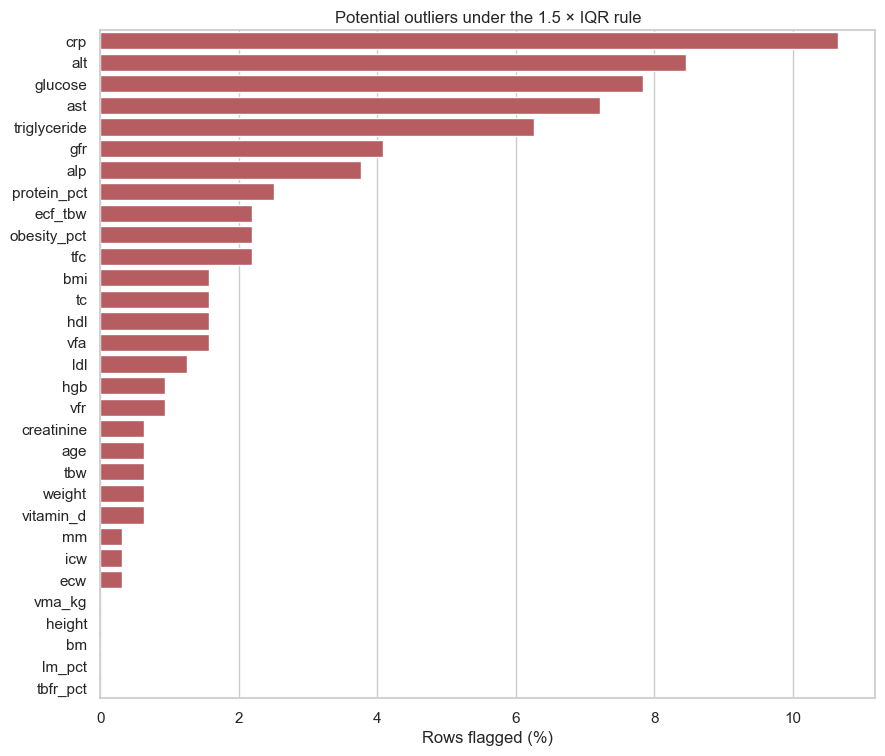
\includegraphics[width=\linewidth]{media/Outlier_Analysis.png}
    \caption{Outlier analysis using the 1.5$\times$IQR method.}
    \label{fig:outlier-analysis}
\end{figure}

Figure~\ref{fig:outlier-analysis} identifies several observations that require further investigation. Most notably, the \textit{Obesity} variable contains an extreme value of approximately 2000, which is substantially larger than the remaining observations. Given the magnitude of this difference, the value should be verified against the original dataset and variable definition to determine whether it represents a valid measurement, a unit inconsistency, or a data-entry error.

Potential upper-tail outliers are also observed in variables including glucose, HDL, triglyceride, AST, ALT, CRP, and intracellular water (ICW). However, observations identified by the 1.5$\times$IQR rule should not automatically be treated as erroneous, particularly in clinical data where extreme measurements may represent genuine patient conditions. Therefore, these observations will be reviewed during data preparation before any correction, transformation, or removal is applied.

Valid extreme observations will be retained where appropriate to preserve clinically meaningful variation in the dataset. Only values supported by evidence of coding, measurement, or data-entry errors will be considered for correction or exclusion. This approach reduces the risk of removing informative clinical cases and introducing bias into subsequent predictive models.


\subsubsection{Dimensionality Reduction Visualisation and Data Understanding}
\label{subsubsec:dimensionality_reduction}

Dimensionality-reduction techniques were used to obtain a more compact view of
the relationships among the continuous measurements and to assess whether
participants with and without gallstones exhibit distinct multivariate patterns.
Two complementary approaches were considered: Principal Component Analysis
(PCA) and t-distributed Stochastic Neighbor Embedding (t-SNE). PCA provides a
linear representation of the dominant sources of variance in the data, whereas
t-SNE is a nonlinear technique designed to preserve local neighbourhood
relationships in a low-dimensional representation
\parencite{vandermaaten2008tsne}.

\paragraph{Principal Component Analysis}

PCA was first applied to the continuous measurements to examine the main
directions of variation in the dataset. The first principal component (PC1)
explained 27.7\% of the total variance, while the second principal component
(PC2) explained a further 20.0\%. Together, the first two components therefore
accounted for approximately 47.7\% of the variance in the continuous feature
space.

\begin{figure}[H]
    \centering
    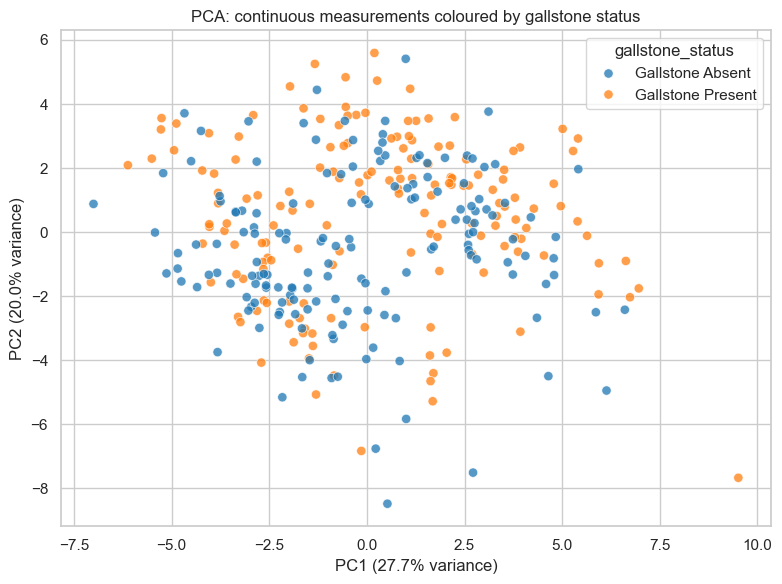
\includegraphics[
        width=0.76\linewidth,
        keepaspectratio
    ]{media/PCA.png}
    \caption{Two-dimensional PCA projection of the continuous measurements,
    coloured by Gallstone Status. PC1 and PC2 explain 27.7\% and 20.0\% of the
    total variance, respectively.}
    \label{fig:pca_projection}
\end{figure}

As shown in Figure~\ref{fig:pca_projection}, observations from the
\textit{Gallstone Present} and \textit{Gallstone Absent} groups overlap
substantially in the first two principal components. No distinct linear
separation between the two outcome groups is apparent. This indicates that the
largest sources of variation in the continuous measurements are not themselves
equivalent to the variation that separates gallstone status.

Nevertheless, the projection reveals meaningful structure within the
measurements. Participants are distributed across several regions of the PCA
space, suggesting heterogeneity in body-composition, anthropometric, and related
clinical characteristics. A small number of observations also lie relatively
far from the central concentration of the data. These observations are
consistent with the unusual or extreme measurements identified during the
earlier univariate exploration and were retained for further investigation
rather than being removed solely on the basis of their position in the PCA
projection.

To understand which variables contribute most strongly to the two principal
components, the corresponding PCA loadings were also examined.

\begin{figure}[H]
    \centering
    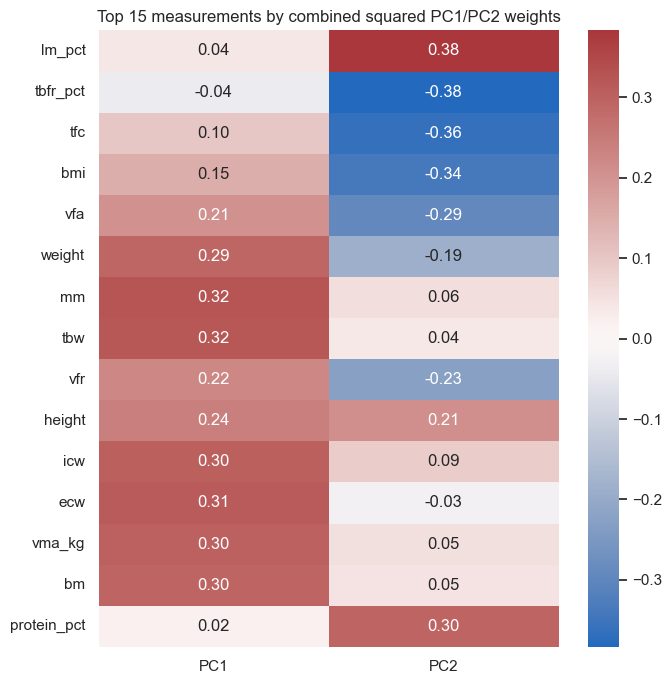
\includegraphics[
        width=0.62\linewidth,
        keepaspectratio
    ]{media/PCA_weight_measurement.png}
    \caption{Loadings of the 15 continuous measurements with the largest
    combined squared contributions to PC1 and PC2. Positive and negative values
    indicate the direction of association with each principal component.}
    \label{fig:pca_loadings}
\end{figure}

Figure~\ref{fig:pca_loadings} shows that PC1 is influenced primarily by several
body-size and body-composition measurements. Muscle mass (\texttt{mm}),
total body water (\texttt{tbw}), extracellular water (\texttt{ecw}),
intracellular water (\texttt{icw}), visceral muscle area
(\texttt{vma\_kg}), bone mass (\texttt{bm}), weight, and height all have
positive loadings on PC1. This suggests that PC1 broadly represents variation
associated with overall body size and lean/body-composition characteristics.

PC2 captures a different contrast. Lean-mass percentage
(\texttt{lm\_pct}) and protein percentage (\texttt{protein\_pct}) have strong
positive loadings, whereas total body-fat percentage (\texttt{tbfr\_pct}),
total fat content (\texttt{tfc}), BMI, visceral fat area (\texttt{vfa}), and
visceral fat rating (\texttt{vfr}) have negative loadings. PC2 can therefore be
interpreted as reflecting a contrast between lean-body composition and
fat-related measurements. These loading patterns provide additional insight into
the correlations among the original measurements and help explain the structure
observed in the PCA projection.

\paragraph{t-SNE Visualisation}

Because PCA represents only linear combinations of the original variables, a
nonlinear t-SNE analysis was additionally performed to examine whether local
neighbourhood structures could reveal patterns that were not visible in the PCA
projection. Multiple perplexity values were evaluated rather than relying on a
single t-SNE configuration.

\begin{figure}[H]
    \centering
    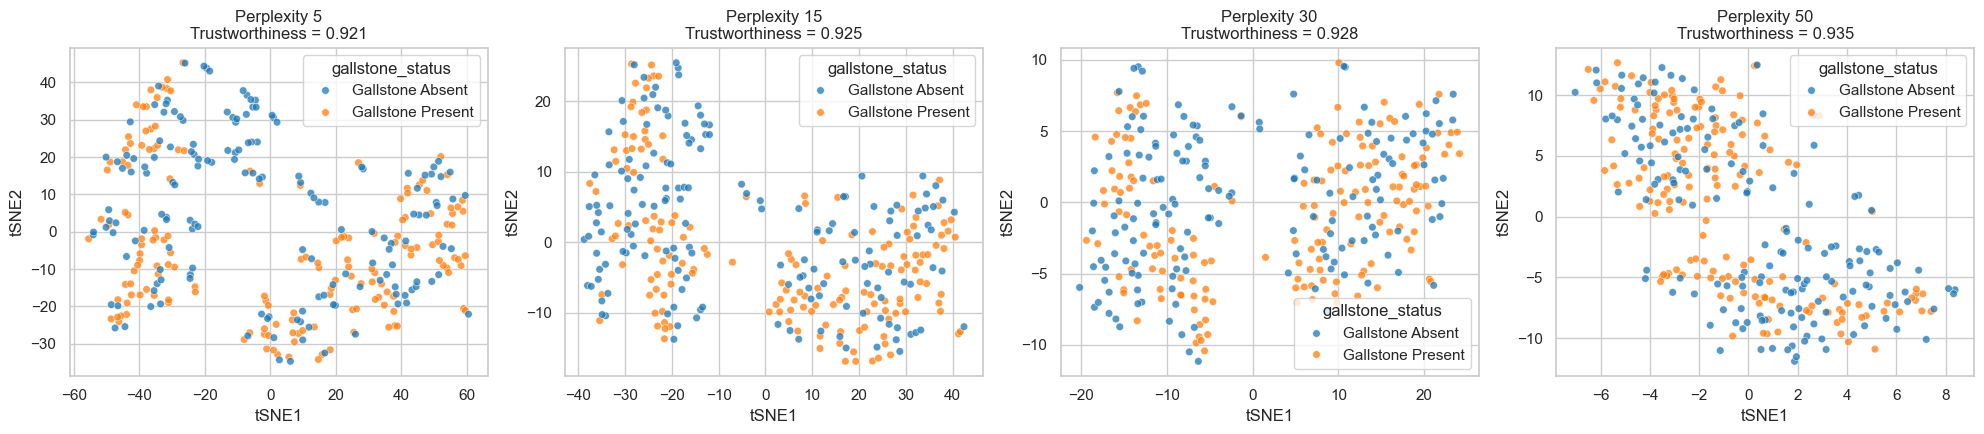
\includegraphics[
        width=\linewidth,
        keepaspectratio
    ]{media/TSNE_visualization.png}
    \caption{Two-dimensional t-SNE projections of the continuous measurements
    using perplexity values of 5, 15, 30, and 50. Points are coloured according
    to Gallstone Status. Trustworthiness scores are reported for each
    configuration.}
    \label{fig:tsne}
\end{figure}

Figure~\ref{fig:tsne} shows that the overall appearance of the t-SNE
representation changes as the perplexity parameter increases. Lower perplexity
values, particularly 5, emphasise very local neighbourhoods and produce a more
fragmented representation. At larger perplexities, the observations form
broader and more coherent structures.

The trustworthiness score increased from 0.921 at perplexity 5 to 0.935 at
perplexity 50, indicating that the higher-perplexity representations preserved
the original local neighbourhood relationships slightly more effectively.
However, the purpose of this metric is to assess preservation of neighbourhood
structure rather than separation of the target classes.

Across all perplexity settings, participants with and without gallstones remain
substantially intermixed. Although some local regions contain a greater
concentration of one class than the other, there is no stable class-specific
cluster or simple visual boundary that consistently separates
\textit{Gallstone Present} from \textit{Gallstone Absent}. The same general
conclusion is therefore observed in both the linear PCA representation and the
nonlinear t-SNE representations.


These findings suggest that gallstone status is unlikely to be explained by a
single dominant measurement or by a simple low-dimensional boundary. Instead,
the predictive information may be distributed across several demographic,
body-composition, metabolic, and biochemical variables and may involve
interactions or nonlinear relationships among them. This observation motivates
the subsequent comparison of multivariable classification models.

Importantly, both PCA and t-SNE were used here as exploratory tools for data
understanding rather than as measures of predictive performance. Visual overlap
between the classes does not imply that the target is unpredictable, since
discriminative information may exist in dimensions that are not represented by
the first two principal components or by the two-dimensional t-SNE embedding.
Model performance is therefore assessed separately using the validation and test
partitions.

% 4. DATA PREPARTION
\section{Data Preparation}
\label{sec:data-preparation}
The purpose of the data-preparation stage was to transform the raw Gallstone
dataset into a consistent, traceable, and modelling-ready dataset. Decisions
made during this stage were informed by the business objective, findings from
the exploratory analysis, data-quality checks, and the technical requirements
of the modelling pipeline.

All data-preparation procedures were implemented using an open-source Python
workflow. The main libraries used were \texttt{pandas} and \texttt{NumPy} for
data manipulation and validation, \texttt{SciPy} for statistical
transformations, \texttt{scikit-learn} for data partitioning and preprocessing,
and \texttt{Matplotlib} and \texttt{Seaborn} for diagnostic visualisation.

Using Python rather than a graphical modelling environment provides a
script-based and reproducible workflow in which each preprocessing operation can
be inspected, rerun, and consistently applied to subsequent modelling
experiments.


\subsection{Data Selection}
\label{subsec:data-selection}

The modelling dataset contains \textit{Gallstone Status} as the target variable
and the available demographic, comorbidity, body-composition, and laboratory
measurements as candidate predictors. Variables were initially retained rather
than removed solely on the basis of weak univariate relationships because the
exploratory analysis suggested that gallstone status may depend on combinations
of multiple patient characteristics.

Data selection was performed programmatically using Python. The dataset was
loaded into a \texttt{pandas DataFrame}, after which column names, data types,
unique values, distributions, and summary statistics were inspected. Candidate
predictors were retained when they had plausible clinical relevance and
sufficient data quality for subsequent modelling.

Variables containing unusual values, strong skewness, or high correlations with
other predictors were not immediately removed. Instead, these characteristics
were investigated during exploratory analysis and preprocessing. In particular,
highly correlated predictors were reviewed during feature selection because
multicollinearity may influence coefficient stability in models such as
logistic regression.

No patient-identifying information or variables without potential predictive
value were required for model development. Identifier fields used for data
traceability were retained during data processing but excluded from the feature
matrix supplied to the predictive models.


\subsection{Data Cleaning}
\label{subsec:data-cleaning}

Data cleaning was guided by the issues identified during the earlier
data-quality assessment. The Python workflow systematically evaluated missing
values, duplicated records, invalid categorical codes, numerical ranges, data
types, and potential extreme observations.

Completeness was assessed using functions such as
\texttt{DataFrame.isna()}, while duplicate observations and field-level
consistency were examined using standard \texttt{pandas} operations. Summary
statistics and value-frequency tables were also generated to identify
unexpected values and inconsistencies.

No missing values were identified in the original dataset; therefore, no
imputation was required before modelling. Nevertheless, missing-value checks
were retained as part of the preprocessing pipeline so that the workflow can
identify incomplete observations if the dataset is modified or extended in
future iterations.

Categorical variables were checked against their documented coding ranges.
Binary and ordinal fields stored numerically were treated according to their
clinical meaning rather than automatically interpreted as continuous
measurements.

Potential outliers were identified during exploratory analysis using the
1.5$\times$IQR rule:

\[
    \mathrm{Lower\ Bound} =
    Q_1 - 1.5(Q_3-Q_1),
\]

\[
    \mathrm{Upper\ Bound} =
    Q_3 + 1.5(Q_3-Q_1).
\]

Observations outside these limits were reviewed rather than automatically
removed. This distinction is important for clinical data because statistically
extreme observations may nevertheless correspond to genuine patient
measurements.

In particular, the unusually large observation identified in the
\textit{Obesity} variable was reviewed as a possible data-quality issue.
Similarly, extreme observations in glucose, triglyceride, AST, ALT, CRP, and
other laboratory measurements were retained when they represented plausible
clinical values. Records would only be corrected or excluded if there were
sufficient evidence of a coding, unit, or data-entry error.

Column names were also standardised programmatically to remove unnecessary
spaces and special characters and to provide consistent variable names
throughout the analysis.


\subsubsection{Cleaning and Sanity-Checking Workflow}

The data-cleaning process was implemented as a reproducible sequence of Python
operations. The main stages were:

\begin{enumerate}
    \item verify the number of observations and variables;
    \item inspect data types and expected variable roles;
    \item identify missing and blank values;
    \item detect duplicate observations;
    \item validate categorical coding ranges;
    \item examine descriptive statistics for continuous measurements;
    \item identify potential extreme observations;
    \item standardise column names and field representations; and
    \item confirm the dimensions and integrity of the resulting analytical
          dataset.
\end{enumerate}

This workflow provided explicit quality-control checkpoints while preserving the
original observations whenever no clear data-quality issue was present.

\subsubsection{Skewness Assessment and Transformation of Continuous Features}
\label{subsubsec:skewness-transformation}

The distributions of the continuous predictors were further examined using
sample skewness to identify variables with substantial departures from
symmetry. Absolute skewness values greater than or equal to 1 were treated as
an indication of strong skewness and were selected for further transformation
assessment.

\begin{figure}[H]
    \centering
    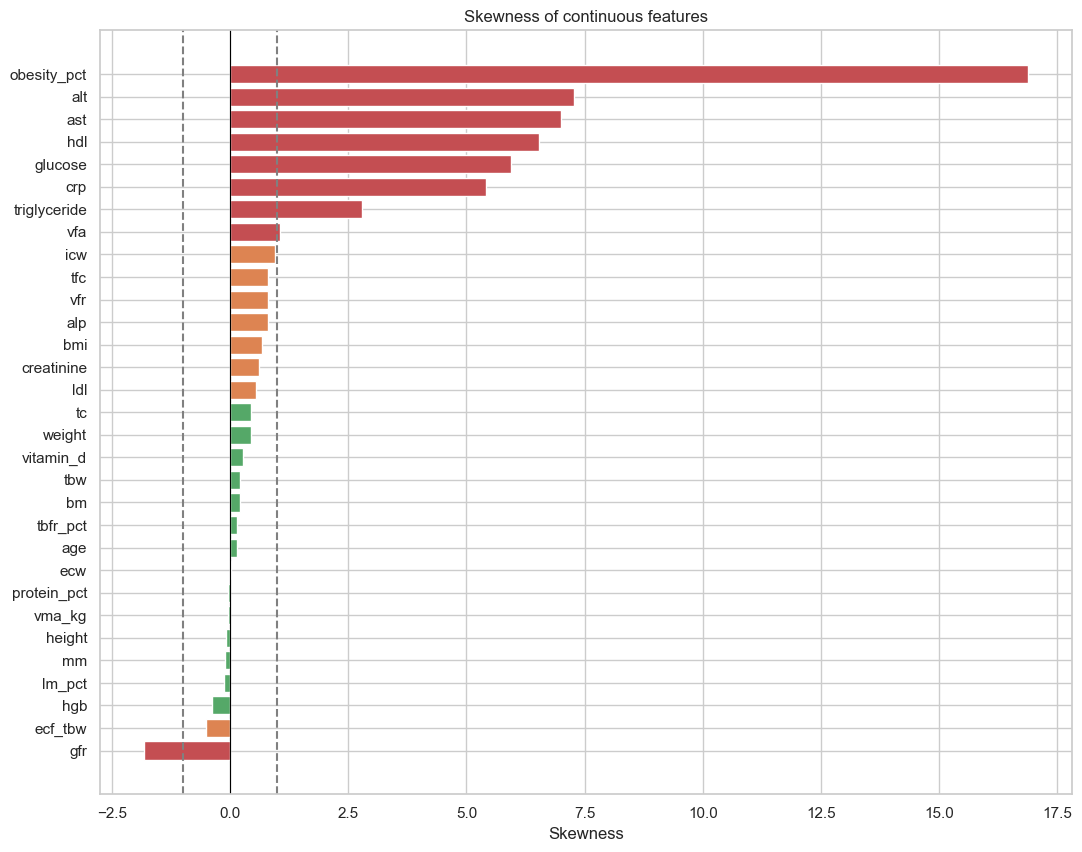
\includegraphics[
        width=0.88\linewidth,
        keepaspectratio
    ]{media/skewness_continous_features.png}
    \caption{Skewness of the continuous variables. The dashed vertical lines
    indicate the threshold of $|\mathrm{skewness}| = 1$ used to identify
    strongly skewed variables.}
    \label{fig:continuous-skewness}
\end{figure}

Figure~\ref{fig:continuous-skewness} shows that several continuous measurements
were strongly right-skewed. The most extreme case was
\texttt{obesity\_pct}, with a skewness of approximately 16.87, followed by
ALT (7.28), AST (6.99), HDL (6.53), glucose (5.94), and CRP (5.41).
Triglyceride was also strongly positively skewed (2.79), while GFR exhibited
substantial negative skewness ($-1.81$). VFA showed a smaller but still notable
positive skewness of approximately 1.06. In contrast, most of the remaining
continuous measurements were relatively close to symmetric.

These results are consistent with the earlier outlier analysis. In particular,
the extreme skewness of \texttt{obesity\_pct} appears to be strongly influenced
by the unusually large observation identified during data-quality assessment.
Similarly, the long right tails observed for ALT, AST, glucose, CRP, and
triglyceride indicate that a small number of participants have measurements
considerably larger than the majority of the sample. These observations were
not removed solely because they increased skewness, since extreme values may
represent clinically plausible measurements.


\subsection{Data Construction}
\label{subsec:data-construction}

The data-construction stage focused on producing a consistent analytical dataset
while preserving the original source data. No additional derived clinical
variables were introduced unless they had a clear analytical justification.

Three logical versions of the dataset were maintained:

\begin{itemize}
    \item \textbf{Raw data:} the original dataset retained without
          modification;

    \item \textbf{Cleaned data:} the dataset after validation of field names,
          data types, categorical values, ranges, duplicates, and potential
          data-quality issues;

    \item \textbf{Model-ready data:} the final analytical dataset containing
          \textit{Gallstone Status} and the predictor variables used by the
          Python modelling pipeline.
\end{itemize}

This separation ensures that preprocessing operations do not overwrite the
source dataset and allows each transformation to be reproduced from the raw
data through the Python scripts.


\subsubsection{Data Partitioning}
\label{subsubsec:data-partitioning}
Before feature selection and model development, two complementary data-splitting
and evaluation strategies were adopted to assess model performance and
robustness: a stratified 70--15--15 holdout split and a
\textit{Leave-One-Patient-Out} (LOPO) cross-validation procedure.

\paragraph{Strategy 1: Stratified 70--15--15 Holdout Split}

For the primary holdout evaluation, the model-ready dataset was partitioned
using the \texttt{scikit-learn} library with stratification based on
\textit{Gallstone Status}. The following proportions were used:

\begin{itemize}

    \item \textbf{70\% Training set:} used for preprocessing decisions,
          feature selection, and model fitting;

    \item \textbf{15\% Validation set:} used for model comparison,
          hyperparameter tuning, threshold analysis, and model-selection
          decisions;

    \item \textbf{15\% Test set:} retained for the final evaluation of the
          selected modelling approach on previously unseen observations.

\end{itemize}

Stratification was used to preserve the approximately balanced distribution of
participants with and without gallstones across the three subsets. This was
particularly important given the relatively small dataset because substantial
differences in class proportions between partitions could otherwise introduce
additional variability into the evaluation results.

The partitioning process can be represented conceptually as follows:

\begin{figure}[H]
    \centering

    \fbox{
        \parbox{0.90\linewidth}{
            \centering

            \textbf{Model-ready Dataset}

            \vspace{0.3cm}

            $\downarrow$

            \vspace{0.3cm}

            \textbf{Stratified Partition by Gallstone Status}

            \vspace{0.4cm}

            \begin{tabular}{ccc}
                \textbf{70\% Training}
                &
                \textbf{15\% Validation}
                &
                \textbf{15\% Test}
                \\[0.2cm]

                Feature selection
                &
                Model comparison
                &
                Final evaluation
                \\

                Model fitting
                &
                Parameter tuning
                &
                Unseen observations
            \end{tabular}
        }
    }

    \caption{Training, validation, and testing strategy used in the Python
    modelling workflow.}
    \label{fig:partition-workflow}
\end{figure}

Feature-selection decisions and model fitting were performed using only the
training partition. The validation partition was subsequently used to compare
candidate models and tune modelling choices. The final test partition remained
separate from these stages and was used only after the modelling strategy had
been established.

\paragraph{Strategy 2: Leave-One-Patient-Out Evaluation}

A second evaluation strategy, referred to as
\textit{Leave-One-Patient-Out} (LOPO), was used to provide an additional
assessment of model robustness on unseen patients. LOPO corresponds to
leave-one-out cross-validation at the patient level. During each iteration, one
patient was held out for evaluation while all remaining patients were used for
model training.

For a dataset containing $N$ patients, the procedure generates $N$ model-fitting
iterations:

\[
\mathcal{D}_{\mathrm{train}}^{(i)}
=
\mathcal{D} \setminus \{P_i\},
\qquad
\mathcal{D}_{\mathrm{test}}^{(i)}
=
\{P_i\},
\]

where $P_i$ denotes the patient excluded from the training data during
iteration $i$.

This process was repeated until every patient had served once as the unseen
evaluation case. The predictions generated across all iterations were then
combined to calculate the overall evaluation metrics.

The LOPO strategy differs from the holdout approach because almost the entire
dataset is available for model fitting during each iteration. This is
particularly useful for the Gallstone dataset because of its relatively small
sample size and provides an assessment of whether the model can generalise to
an individual patient who was completely excluded from the corresponding
training process.

The two strategies were evaluated separately. The 70--15--15 split provides a
conventional development framework with independent training, validation, and
test partitions, while LOPO evaluates model stability and patient-level
generalisation across the complete dataset. Using both approaches provides a
more comprehensive assessment of predictive performance than relying on a
single data split alone.

These separation reduces the risk of information leakage and provides a more
independent estimate of how well the resulting model is expected to generalise
to previously unseen patient observations.

Any preprocessing operation that required parameters to be estimated from the
data was fitted using the training partition only and subsequently applied to
the validation and test partitions. This principle applies, for example, to
feature scaling, statistical transformations, and model-based feature
selection.


\subsection{Data Integration}
\label{subsec:data-integration}

Although the Gallstone dataset was originally obtained as a single public
dataset, an explicit integration exercise was conducted to demonstrate how
logically separate healthcare data sources can be combined into a unified
analytical table.

The original dataset was preserved unchanged and divided into two logical CSV
sources. The first file,
\texttt{gallstone\_demographic\_clinical.csv}, contains 319 records and
9 fields describing demographic and clinical characteristics. The second file,
\texttt{gallstone\_biological\_body\_composition.csv}, contains the same
319 participants and 33 fields describing biological, laboratory, and
body-composition measurements.

A unique \texttt{record\_id}, ranging from 1 to 319, was included in both
tables as the one-to-one integration key. Both tables also contained
\textit{Gallstone Status} so that target consistency could be verified before
integration. However, \textit{Gallstone Status} was not used as a merge key
because it does not uniquely identify an individual participant.

Integration was implemented using the \texttt{pandas.merge()} operation with
\texttt{record\_id} as the matching field. The merge was configured as a
one-to-one operation so that duplicate identifiers or unexpected many-to-one
relationships could be detected explicitly.

Post-integration quality checks verified that all 319 participant records were
retained and that no unmatched identifiers or additional missing values were
introduced by the merge.

The duplicated \textit{Gallstone Status} fields from the two logical data
sources were compared before one copy was removed from the final analytical
table. The \texttt{record\_id} field was retained for traceability and quality
control but excluded from the predictor set used for model development.

This integration exercise represents a simplified version of a realistic
healthcare environment in which demographic and clinical data may be stored
separately from laboratory or body-composition measurements. The Python
workflow demonstrates how these sources can be integrated while maintaining
record integrity and preventing inappropriate use of the target variable as an
integration key.


\subsection{Data Reformatting}
\label{subsec:data-reformatting}

The original Gallstone dataset was provided in Microsoft Excel format
(\texttt{.xlsx}). The file was loaded programmatically using
\texttt{pandas.read\_excel()} and subsequently exported to comma-separated
values (\texttt{.csv}) where appropriate for intermediate storage and
reproducible processing.

CSV was selected as an intermediate format because it provides a simple,
platform-independent representation of tabular data and avoids spreadsheet
formatting that is irrelevant to the modelling process. The use of CSV was not
a modelling requirement, however, because the Python pipeline can also operate
directly on Excel or other structured tabular formats.

During reformatting, variable names were standardised and unnecessary
spreadsheet-specific formatting was removed. The resulting fields were then
classified according to their analytical meaning.

Continuous clinical and body-composition measurements, such as BMI, glucose,
triglyceride, weight, and total body water, were represented as numerical
variables.

Binary variables such as Coronary Artery Disease, Hypothyroidism,
Hyperlipidemia, and Diabetes Mellitus were stored as categorical or binary
indicators rather than being interpreted as continuous measurements.

Variables representing ordered clinical levels were treated as ordinal
variables when their coding reflected an increasing degree of severity or
disease burden.

The target variable, \textit{Gallstone Status}, was represented internally as a
binary label for model training while human-readable labels
(\textit{Gallstone Absent} and \textit{Gallstone Present}) were used in
tables and visualisations.

The final model-ready dataset therefore contained consistent field names,
validated data types, clearly defined variable roles, and a reproducible schema
that could be used directly by the subsequent Python-based feature engineering
and modelling pipeline.


\subsection{Reproducible Open-Source Preparation Pipeline}
\label{subsec:python-preparation-pipeline}

The complete preparation process was implemented as a script-based
open-source workflow. At a high level, the pipeline consisted of:

\begin{enumerate}
    \item loading the source data using \texttt{pandas};
    \item standardising variable names and data types;
    \item validating missing values, duplicates, coding ranges, and
          observations;
    \item performing exploratory outlier and distribution checks;
    \item integrating logically separated datasets using
          \texttt{pandas.merge()};
    \item constructing the final predictor and target datasets;
    \item creating stratified training, validation, and test partitions using
          \texttt{scikit-learn};
    \item fitting any required preprocessing operations using the training
          subset only; and
    \item passing the resulting datasets to the machine-learning modelling
          pipeline.
\end{enumerate}

The use of an open-source Python stack provides several advantages for this
project. Each operation is explicitly defined in code, preprocessing decisions
can be version-controlled, experiments can be reproduced using fixed random
seeds, and identical transformations can be consistently applied across
multiple candidate models.

The resulting workflow therefore provides a transparent and reproducible
transition from the original Gallstone dataset to the datasets used for model
training, validation, and final evaluation.

\subsection{Data Reduction and Projection}
\label{sec:data-reduction}
\subsubsection{Feature Selection and Horizontal Data Reduction}
\label{subsec:feature-selection}

Horizontal data reduction was performed to retain predictors that provide useful information for predicting \textit{Gallstone Status}, while reducing
unnecessary or weakly informative inputs. This was particularly relevant
because the exploratory analysis identified substantial correlation among
several body-composition and laboratory measurements.

\paragraph{Random Forest Feature Importance}
\label{subsubsec:random-forest-importance}

A Random Forest classifier was used as an exploratory feature-ranking method.
Random Forests combine multiple decision trees constructed from bootstrap
samples and random subsets of predictors, allowing nonlinear relationships and
interactions among variables to be captured without requiring strong parametric
assumptions \parencite{breiman2001randomforests}.

Feature importance was calculated using the impurity-based importance measure provided by the RandomForestClassifier implementation in
\texttt{scikit-learn}\footnote{The implementation and definition of
\texttt{feature\_importances\_} are documented in the scikit-learn
\texttt{RandomForestClassifier} API:
\url{https://scikit-learn.org/stable/modules/generated/sklearn.ensemble.RandomForestClassifier.html}.}.

For each predictor, the importance reflects its normalised contribution to the
total reduction in the splitting criterion across the trees in the forest.
The reported values were averaged across the repeated holdout splits, with the
error bars indicating variability in importance across the different random
seeds.

\begin{figure}[H]
    \centering
    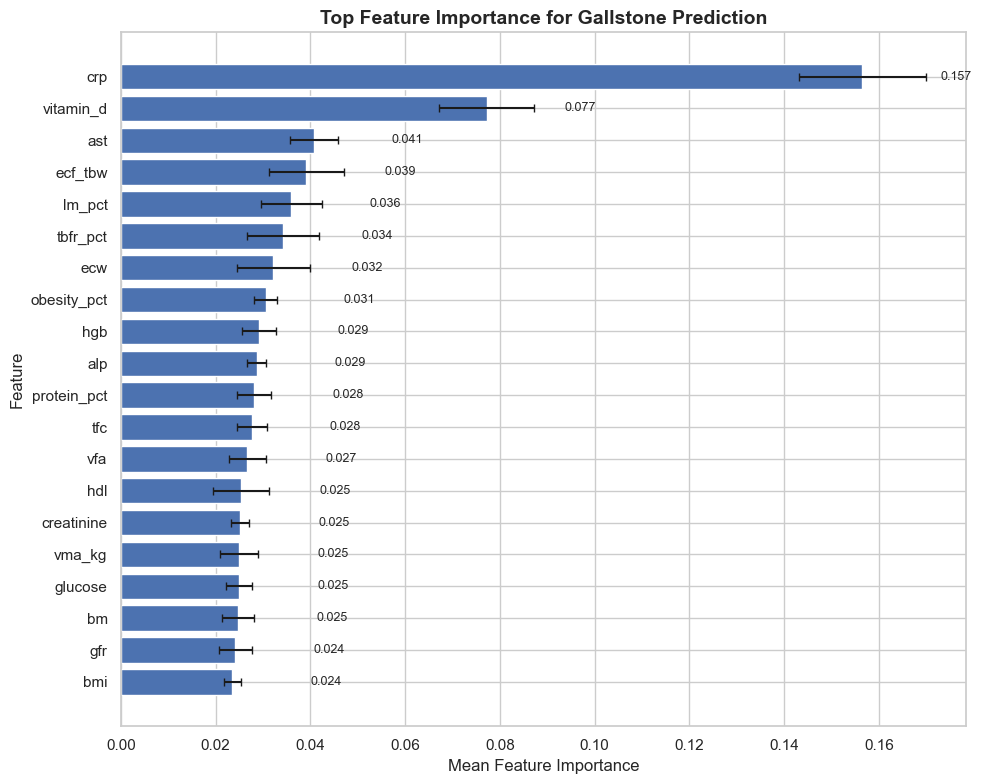
\includegraphics[
        width=0.82\linewidth,
        keepaspectratio
    ]{media/RF_feature_importances.png}
    \caption{Mean Random Forest feature importance for Gallstone Status
    prediction across repeated stratified holdout splits. Error bars represent
    the variability of feature importance across random seeds.}
    \label{fig:random-forest-importance}
\end{figure}

As shown in Figure~\ref{fig:random-forest-importance}, CRP was the most
influential predictor, with a mean importance of approximately 0.157. This was
followed by Vitamin D (0.077), AST (0.041), ECF/TBW (0.039), lean-mass
percentage (0.036), and total body-fat percentage (0.034). ECW,
\texttt{obesity\_pct}, haemoglobin, ALP, protein percentage, total fat content,
VFA, HDL, creatinine, glucose, GFR, and BMI also contributed to the model, but
with smaller individual importance scores.

The ranking suggests that the predictive information is distributed across
multiple clinical domains rather than being dominated by a single type of
measurement. In particular, inflammatory and biochemical variables such as CRP,
AST, and Vitamin D appear alongside body-composition measurements such as
ECF/TBW, lean-mass percentage, total body-fat percentage, ECW, and VFA. This
supports the earlier exploratory findings that Gallstone Status is associated
with a multivariable pattern rather than a simple separation based on one
predictor.

The Random Forest ranking was used as an exploratory assessment of predictor
relevance rather than as the sole criterion for feature removal. Impurity-based
importance can favour variables that provide more potential split points, and
importance values should therefore be interpreted as model-specific indicators
rather than direct measures of clinical effect \parencite{pedregosa2011scikit}.
Final feature-selection decisions were evaluated separately using recursive
feature elimination and predictive performance across the validation
procedures.


\paragraph{Feature Selection After Transformation}
\label{subsubsec:post-transform-selection}

Following the statistical transformation stage, feature selection was performed
using the open-source Python modelling stack. Both the original predictors and
the transformed representations were included as candidate inputs so that the
usefulness of each representation could be evaluated empirically rather than
assuming that transformation would automatically improve prediction.

Horizontal data reduction was performed using Recursive Feature Elimination
(RFE) with a CART decision-tree classifier as the underlying estimator. CART
provides a nonlinear feature-ranking mechanism based on reductions in node
impurity, while RFE recursively removes the least informative predictors and
re-fits the estimator on the remaining feature set. This procedure therefore
reduces the dimensionality of the modelling dataset while retaining variables
that contribute most strongly to the separation of
\textit{Gallstone Present} and \textit{Gallstone Absent} cases.

Feature selection was performed within the training partition for each random
seed to avoid using information from the validation or test data. The resulting
feature rankings were then compared across repeated holdout splits to assess the
stability of the selected predictors.

\begin{figure}[H]
    \centering
    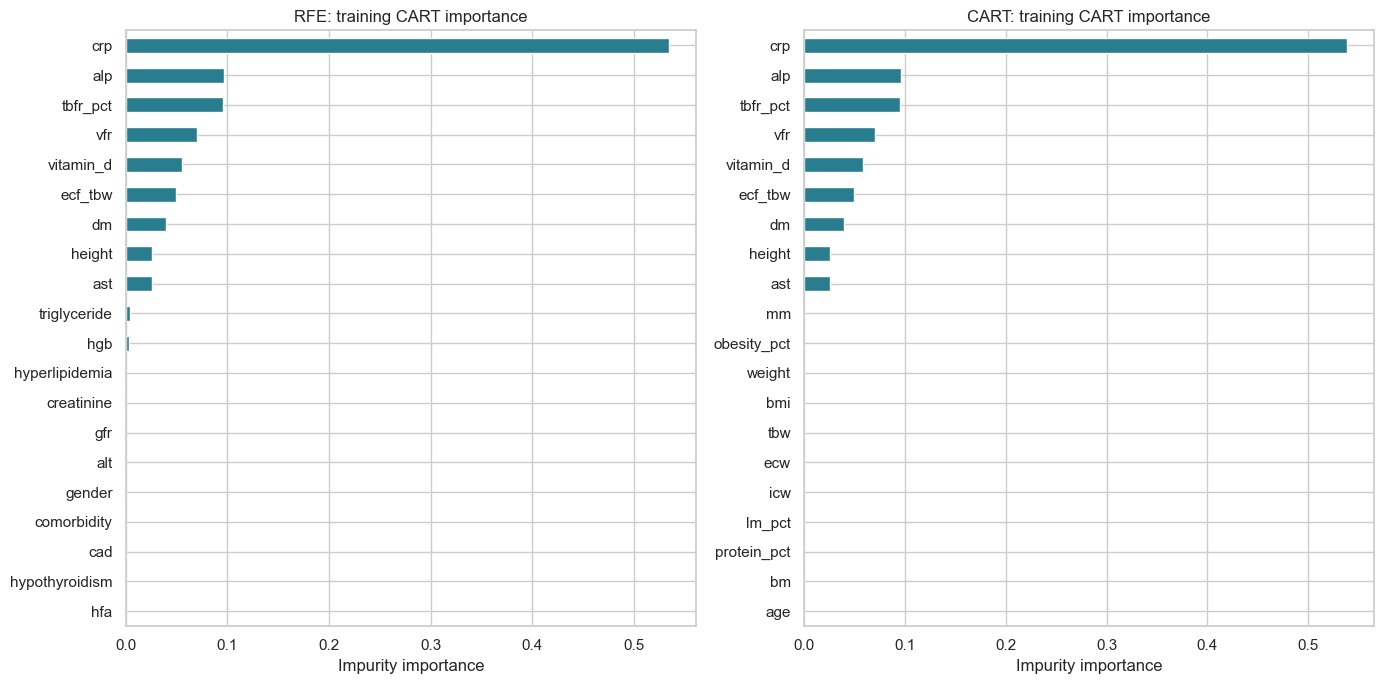
\includegraphics[
        width=0.95\linewidth,
        keepaspectratio
    ]{media/RFE_CART_FE.png}
    \caption{CART-based feature importance used within the recursive feature
    elimination procedure. Predictor importance was estimated using the
    training data only.}
    \label{fig:rfe-cart-importance}
\end{figure}

As shown in Figure~\ref{fig:rfe-cart-importance}, CRP was the dominant predictor
in the CART-based ranking. ALP and total body-fat percentage
(\texttt{tbfr\_pct}) formed the next most influential group, followed by
visceral fat rating (\texttt{vfr}), Vitamin D, ECF/TBW, and diabetes mellitus
(\texttt{dm}). Several additional variables, including height and AST,
contributed more weakly to the fitted tree.

The dominance of CRP was also visible in the individual CART structures. In the
two example training splits shown in Figures~\ref{fig:cart-seed7} and
\ref{fig:cart-seed42}, CRP was selected as the root split, while subsequent
branches incorporated different combinations of body-composition and clinical
variables such as bone mass, ECF/TBW, total body-fat percentage, Vitamin D,
VFR, BMI, and ALP.

\begin{figure}[H]
    \centering
    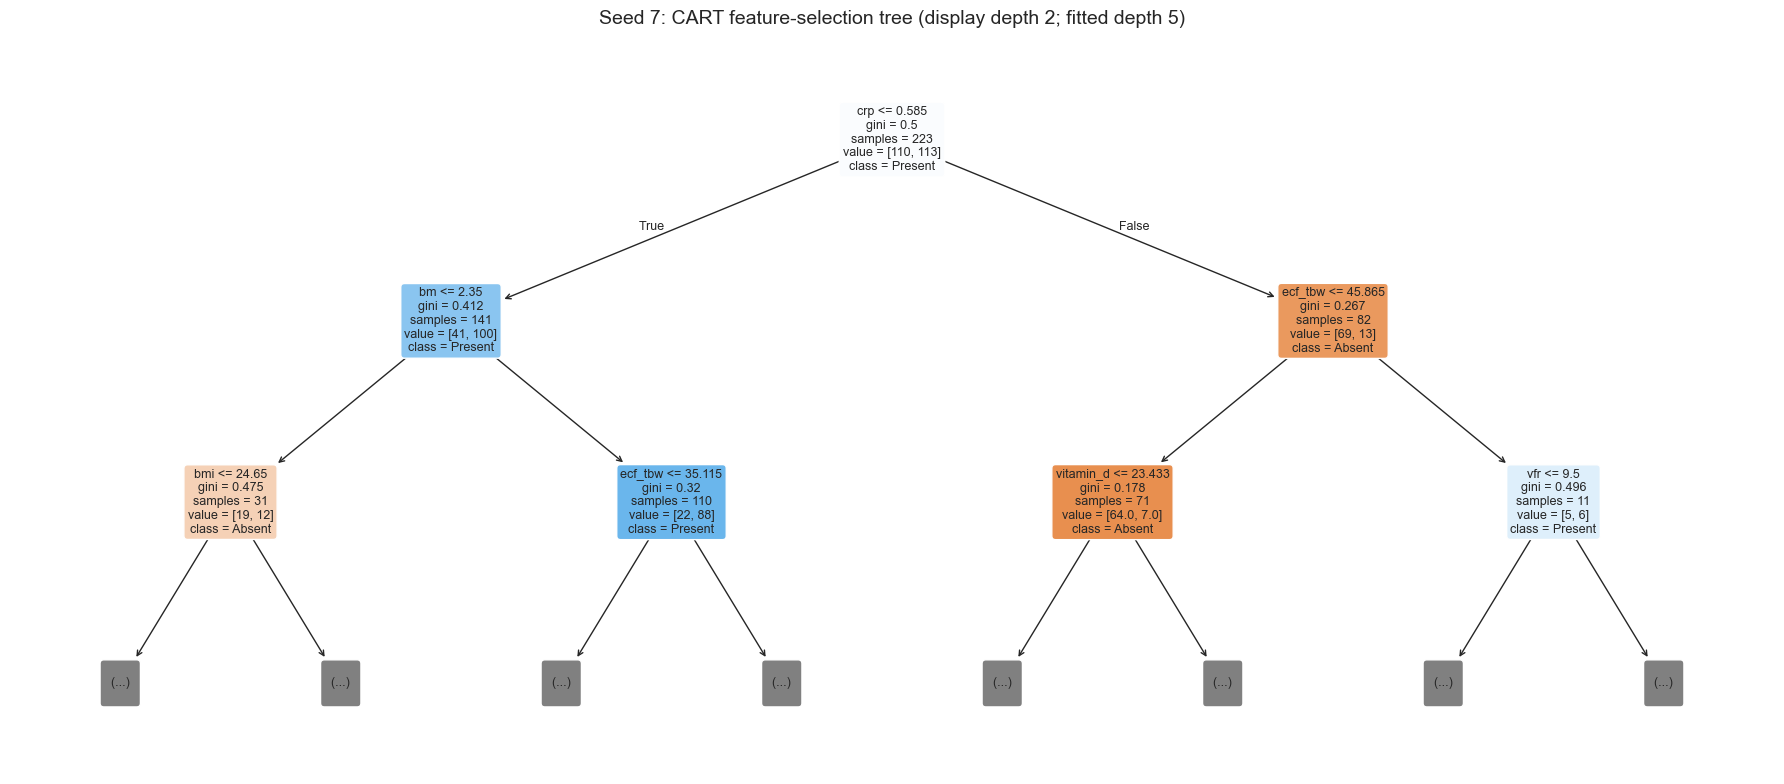
\includegraphics[
        width=\linewidth,
        keepaspectratio
    ]{media/CART_Tree_2.png}
    \caption{Example CART feature-selection tree for one training split. Only
    the upper levels of the fitted tree are displayed for interpretability.}
    \label{fig:cart-seed7}
\end{figure}

\begin{figure}[H]
    \centering
    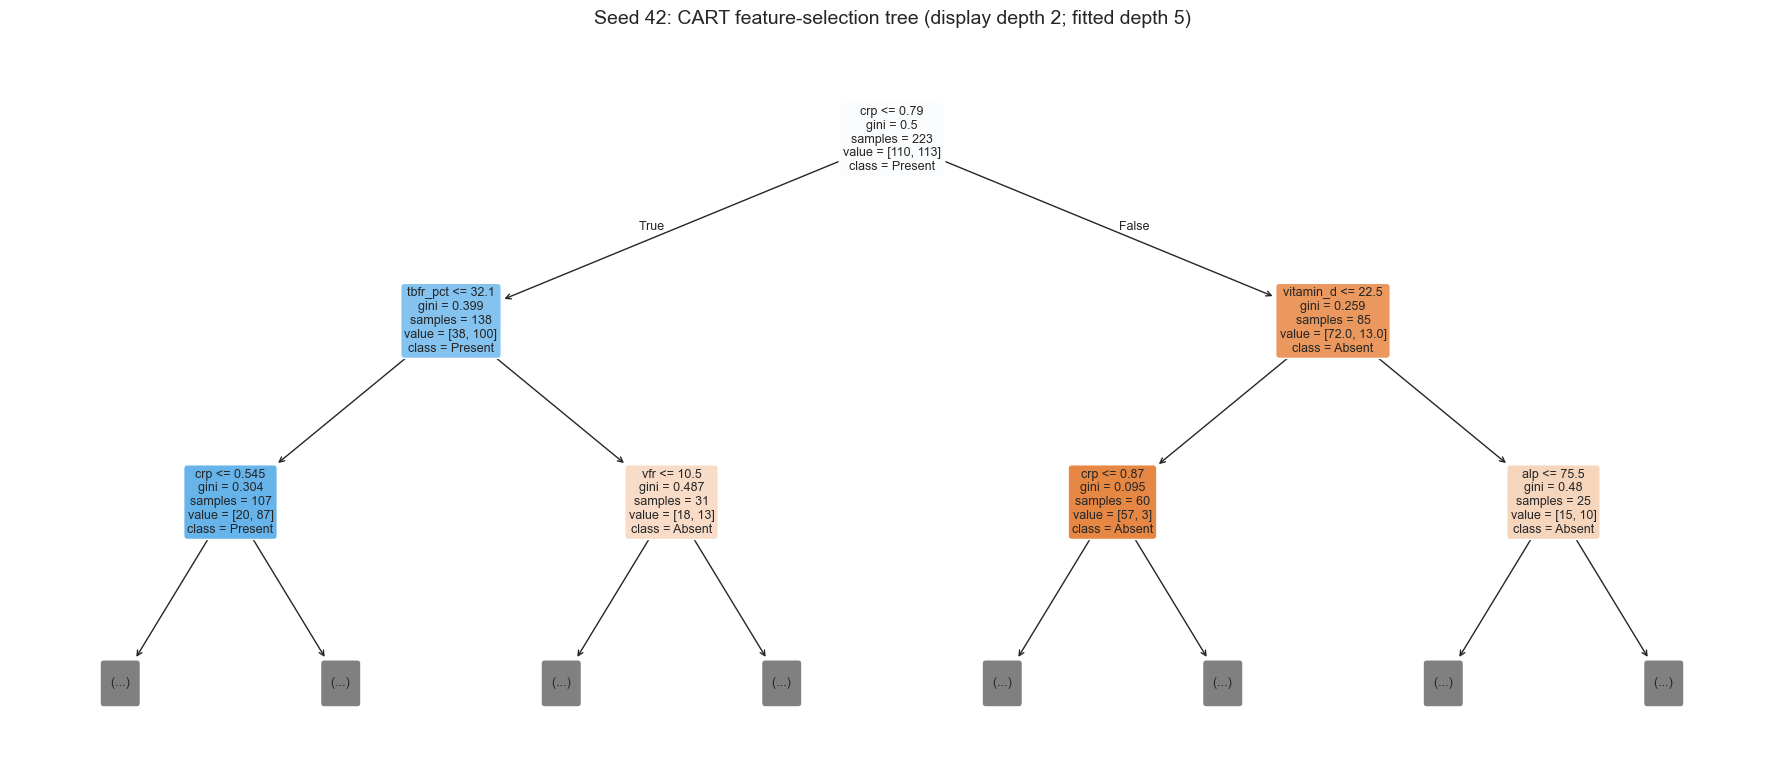
\includegraphics[
        width=\linewidth,
        keepaspectratio
    ]{media/CART_Tree_1.png}
    \caption{Example CART feature-selection tree from a second training split,
    illustrating variation in lower-level splits while retaining CRP as the
    primary separating feature.}
    \label{fig:cart-seed42}
\end{figure}

The variation in the lower branches across training splits indicates that the
dataset does not depend on a single fixed decision rule. Instead, several
clinical and body-composition variables provide complementary information.
Variables appearing repeatedly across the RFE rankings and CART structures were
therefore considered more stable candidates than variables selected only in a
single split.

The final number of predictors was not determined using an arbitrary importance
threshold. Instead, progressively reduced top-$k$ feature subsets generated by
RFE were evaluated on the validation data, and the number of retained features
was selected according to predictive performance across the repeated splits.
This provides a direct link between feature reduction and out-of-sample model
performance.

Together with the preceding transformation stage, this procedure addresses two
forms of data preparation. Statistical transformations project strongly skewed
measurements into alternative numerical representations, while RFE and CART
provide horizontal reduction by removing predictors that contribute limited
additional information. The resulting reduced feature set was subsequently
carried forward to model development and compared with the broader predictor
set.

\paragraph{Vertical Reduction.}
No vertical reduction was applied to the dataset. The available sample contains only 319 observations, so removing records without a clear data-quality reason could unnecessarily reduce the amount of information available for training and evaluation. In addition, the target variable is
already well balanced, with 161 observations representing gallstones present and 158 representing gallstones absent. The exploratory analysis therefore provided no evidence that undersampling or other record-reduction techniques
were required.

All valid observations were consequently retained, while stratified partitioning was used to preserve the target distribution across the
training, validation, and test sets. Data reduction in this project instead
focused on \textit{horizontal reduction}, where feature-selection methods were
used to identify and retain predictors that were most relevant to \textit{Gallstone Status}.

\subsubsection{Statistical Transformation}
\label{subsec:data-transformation}

Exploratory analysis identified substantial skewness in several continuous
predictors, particularly \texttt{obesity\_pct}, ALT, AST, HDL, glucose, CRP,
triglyceride, GFR, and VFA. Rather than transforming all numerical variables,
transformation was considered only for features with
$|\mathrm{skewness}| \geq 1$.

Two transformation approaches were evaluated: the logarithmic transformation
and the Yeo--Johnson power transformation. Their effectiveness was assessed by
comparing the resulting distributions and sample skewness with the original
measurements.

\begin{figure}[H]
    \centering
    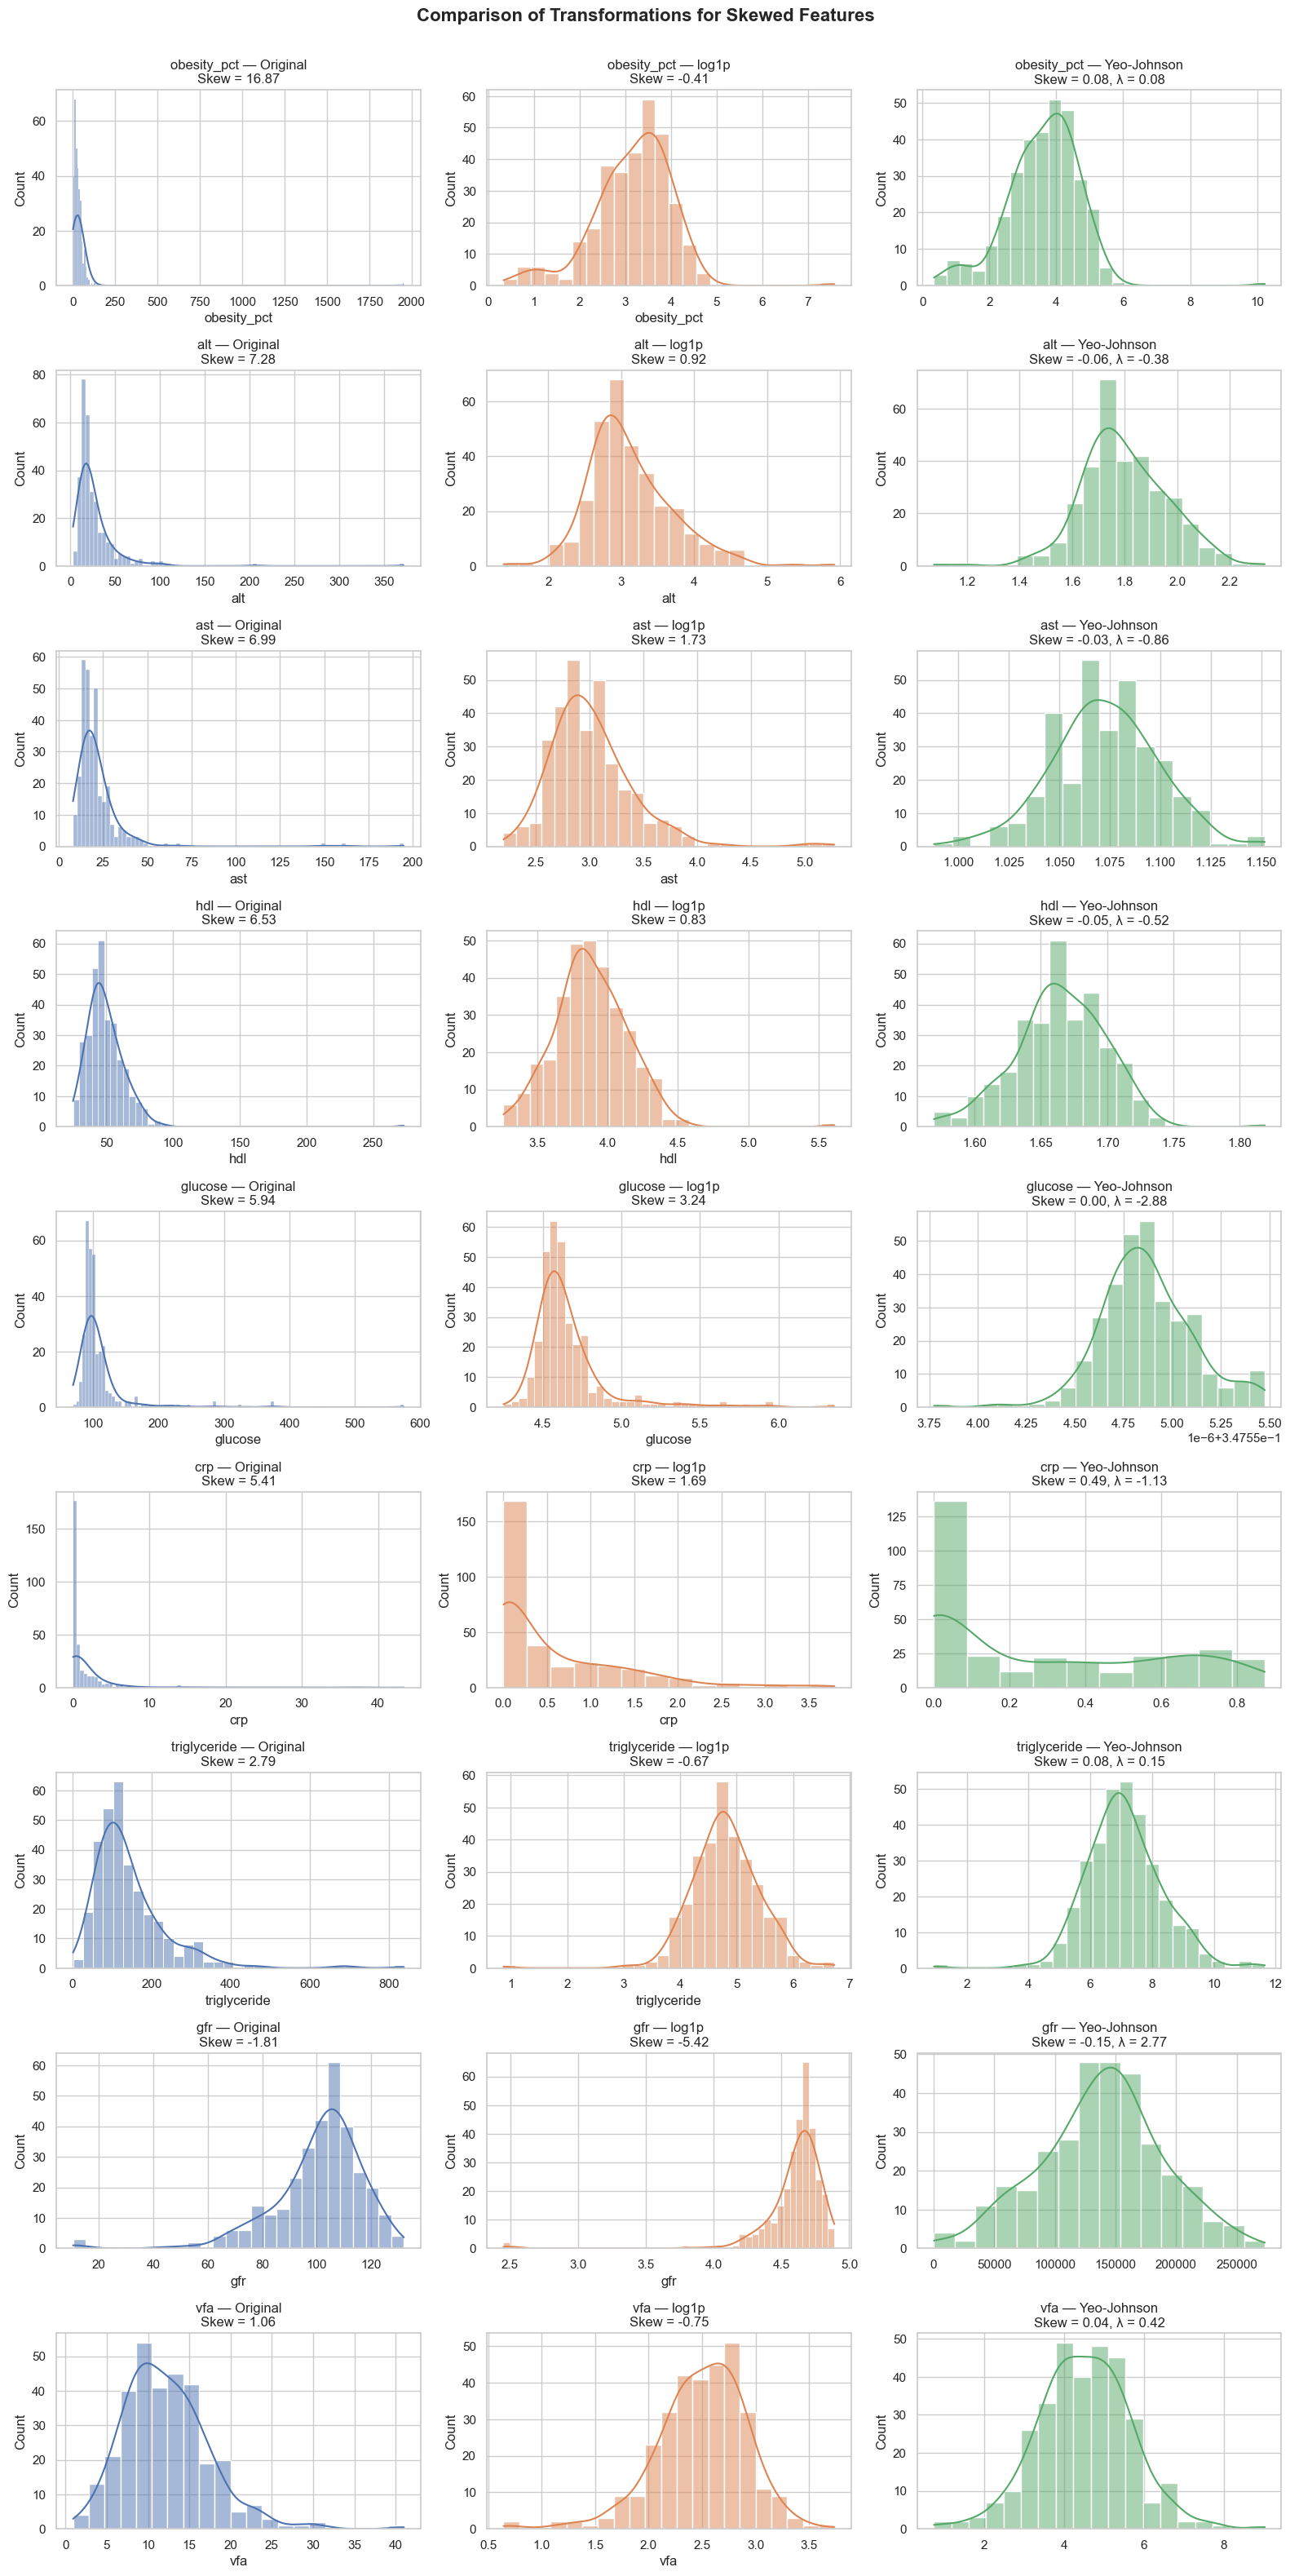
\includegraphics[
        width=\linewidth,
        height=0.88\textheight,
        keepaspectratio
    ]{media/transformation_exetrme.png}
    \caption{Comparison of the original, \texttt{log1p}, and Yeo--Johnson
    distributions for continuous variables with absolute skewness greater than
    or equal to 1. Reported values show the resulting skewness and the estimated
    Yeo--Johnson parameter $\lambda$.}
    \label{fig:transformation-comparison}
\end{figure}


\paragraph{Logarithmic Transformation}
\label{subsubsec:log-transformation}

For non-negative variables, a logarithmic transformation was evaluated using

\[
x_{\mathrm{log}} = \log(1+x),
\]

where the addition of one allows zero-valued observations to be retained.

As shown in Figure~\ref{fig:transformation-comparison}, the transformation
substantially reduced positive skewness for several variables. For example,
the skewness of \texttt{obesity\_pct} decreased from 16.87 to approximately
$-0.41$, while ALT decreased from 7.28 to 0.92 and triglyceride from 2.79 to
0.67. However, the improvement was not consistent across all predictors.
Glucose, for example, remained noticeably right-skewed after transformation,
with skewness decreasing from 5.94 to 3.24.

The logarithmic transformation was therefore treated as a feature-specific
preprocessing option rather than being applied uniformly to all continuous
variables.


\paragraph{Yeo--Johnson Transformation}
\label{subsubsec:yeojohnson-transformation}

The Yeo--Johnson transformation was also evaluated as a more flexible power
transformation. Unlike conventional logarithmic or Box--Cox transformations,
the Yeo--Johnson method can accommodate zero and negative values while
estimating an appropriate transformation parameter, $\lambda$, from the data
\parencite{yeo2000new}.

The transformation is defined piecewise according to the value of $x$ and the
estimated parameter $\lambda$, allowing the shape of the transformation to
adapt to each variable. This makes it particularly useful when continuous
predictors differ substantially in scale and distribution.

Figure~\ref{fig:transformation-comparison} shows that Yeo--Johnson generally
produced stronger reductions in absolute skewness for the most asymmetric
variables. For example, skewness decreased from 16.87 to approximately 0.08
for \texttt{obesity\_pct}, from 7.28 to $-0.06$ for ALT, from 6.99 to 0.03
for AST, and from 5.94 to approximately 0.00 for glucose. Triglyceride was
similarly reduced from 2.79 to approximately 0.08.

These results indicate that Yeo--Johnson provided a more consistent
normalisation of strongly skewed predictors than the logarithmic
transformation for this dataset. Nevertheless, improved symmetry alone was not
used as sufficient justification for retaining a transformed feature.
Transformed and original representations were subsequently evaluated through
feature selection and predictive model performance.


\paragraph{Transformation within the Modelling Pipeline}
\label{subsubsec:transformation-pipeline}

Transformations were implemented as part of the modelling pipeline rather than
as permanent modifications to the source data. Original measurements were
retained for traceability, while transformation parameters were estimated using
the training data only and then applied unchanged to the corresponding
validation and test partitions.

This procedure prevents information from held-out observations from influencing
preprocessing decisions and reduces the risk of data leakage. The final choice
between original and transformed representations was therefore based on both
distributional improvement and downstream predictive performance rather than on
normality alone.



\section{Data-Mining Method Selection}
\label{sec:dm-method-selection}
\subsection{Learning Paradigm and Research Objective}
\label{subsec:matching-dm-methods}

The objective is to estimate gallstone presence from demographic, clinical,
laboratory, and body-composition measurements. All 319 records have a known
binary outcome, making \textbf{supervised learning} the appropriate primary
paradigm: predictions can be compared with observed labels on held-out records.
\textbf{Unsupervised learning} can reveal structure without those labels, but
similarity between patients does not necessarily correspond to disease
status. It therefore supports exploration rather than providing the principal
answer to the research question.

\subsection{Comparison of Data-Mining Methods}
\label{subsec:dm-family-comparison}

The learning paradigm must be narrowed to a method whose output matches the
objective. Table~\ref{tab:dm-family-comparison} distinguishes this decision
from the choice of a particular algorithm.

\begin{table}[H]
\centering
\small
\caption{Suitability of data-mining methods for the gallstone-prediction objective.}
\label{tab:dm-family-comparison}
\begin{tabularx}{\textwidth}{@{}p{2.8cm}XX@{}}
\toprule
Method & Intended output & Suitability for this project \\
\midrule
\textbf{Classification} &
A known class and, where supported, its probability. &
Directly matches labelled gallstone presence/absence and permits evaluation
of discrimination, missed cases, and false alarms. Selected as the primary
method. \\
Continuous-value prediction (regression) &
A numerical quantity, such as a laboratory concentration or severity score. &
The target is a category, not a continuous measurement. This would answer a
different question. Classification is also predictive; the distinction here
concerns the type of output. \\
Segmentation (clustering) &
Groups of observations with similar predictor profiles. &
Useful for exploratory subgroups, but groups need not correspond to
gallstone status. Cluster membership alone is not a validated disease
prediction. \\
Association discovery &
Frequently co-occurring conditions or measurement patterns. &
Useful for hypothesis generation, but support and confidence do not establish
held-out discrimination or an acceptable false-negative rate. Outcome-directed
rules would still require supervised classification evaluation. \\
Anomaly detection &
Observations that differ from a reference pattern. &
Supports review of unusual measurements, but gallstone cases comprise roughly
half the sample and cannot be equated with anomalies. \\
\bottomrule
\end{tabularx}
\end{table}

Dimensionality reduction and feature selection are supporting preparation
methods, not substitutes for predicting the labelled outcome. Likewise,
forecasting future onset or modelling time to diagnosis would require
longitudinal or event-time information not used by the current workflow.
The available evidence supports classification of recorded gallstone status,
not a demonstrated forecast of future disease.

\subsection{Selected Method and Success Criteria}
\label{subsec:dm-method-decision}

The selected method is \textbf{supervised binary classification with
probability estimation}. It provides the required patient-level output and
directly supports the project benchmarks of ROC--AUC at least 0.80 and
gallstone-class sensitivity at least 0.80. Specificity, precision, F1,
stability, and interpretability are needed alongside these measures: predicting
every patient as positive could satisfy sensitivity while producing
unacceptable false alarms.

The source coding is 0 = gallstones present and 1 = absent. The Python
modelling target is recoded to 1 = present and 0 = absent, so
$\mathrm{FNR}=\mathrm{FN}/(\mathrm{FN}+\mathrm{TP})=1-\mathrm{sensitivity}$
measures missed gallstone cases. These are analytical project benchmarks,
not clinical deployment thresholds. The following section compares algorithms
within this chosen method and explains how the implemented models are built
and selected.


\section{Algorithm Selection and Parameterisation}
\label{sec:algorithm-selection}
\subsection{Range of Classification Algorithms}
\label{subsec:algorithm-exploration}

Having selected supervised classification, the next question is which
algorithm offers an appropriate balance of discrimination, case detection,
and interpretability for a small tabular dataset.
Table~\ref{tab:classification-algorithms} distinguishes the algorithms
implemented in the Python experiments from alternatives considered on
methodological grounds. Unimplemented alternatives are not claimed to have
been empirically outperformed.

\begin{table}[H]
\centering
\small
\caption{Algorithm-level exploration within supervised classification.}
\label{tab:classification-algorithms}
\begin{tabularx}{\textwidth}{@{}p{2.7cm}XX@{}}
\toprule
Algorithm & Strength and limitation & Role in this iteration \\
\midrule
Logistic regression &
Regularised, interpretable probability model; its additive form can miss
interactions unless represented in the predictors. &
Implemented as the principal baseline. Despite its name, it models a binary
class probability here. \\
Decision trees: CART &
Readable nonlinear rules, but individual trees can be unstable and overfit
small samples. &
CART is used for feature selection; \\
Random forest &
Combines trees to model interactions; less transparent than a single tree,
with potentially misleading impurity importance for correlated predictors. &
Implemented as the bagged-tree alternative. \\
XGBoost and LightGBM &
Boosted trees can capture nonlinear structure; complexity requires control
through tree size, learning rate, and regularisation. &
Both implemented with bounded settings and tuning grids. \\
Support vector machine &
Linear or kernel boundaries offer alternatives to additive probabilities;
scaling, kernel choice, and probability estimation add decisions. &
Considered but not implemented in this bounded Python comparison. Earlier
test-set LSVM results are not a selection justification. \\
$k$-nearest neighbours and naive Bayes &
Neighbour methods are sensitive to scaling and redundant dimensions;
naive Bayes is simple but assumes conditional independence. &
Not implemented; correlated measurements make their assumptions or distance
representation worth further investigation rather than automatic adoption. \\
Neural network &
Can represent complex interactions, but adds architecture and optimisation
choices and is harder to interpret. &
Deferred given the sample size and scope; no claim that it cannot perform
competitively. \\
Stacking &
Combines complementary model probabilities; requires out-of-fold training
and increases fitting and explanation costs. &
Implemented using the four individual predictive models and a logistic
meta-classifier. \\
\bottomrule
\end{tabularx}
\end{table}

This candidate set tests whether nonlinear models or their combination improve
on the simpler baseline. A training-prior dummy classifier provides a
feature-free benchmark. Unsupervised algorithms are not additional candidates
for the final classifier; their exploratory role is established in
Section~\ref{subsec:dm-family-comparison}.

\subsection{Model Construction Protocol}
\label{subsec:python-candidate-construction}

The Open Source Software Stack uses Python/Jupyter, pandas and NumPy,
scikit-learn, XGBoost, LightGBM, and plotting libraries. Shared
\path{utils.py} and \path{modeling.py} functions support the transformation,
holdout, leave-one-out, tuning, and error-analysis notebooks.

Five label-stratified splits (seeds 42, 7, 21, 84, and 123) each produce
223 training, 48 validation, and 48 test rows. Within training, continuous
measurements are median-imputed and categorical fields most-frequent-imputed.
RFE with CART or direct CART importance selects 20 source predictors, followed
by Yeo--Johnson and standardisation for continuous fields and one-hot encoding
for categories. CART selection uses maximum depth 5 and minimum leaf size 4;
RFE removes one feature per step. The complete preparation is refitted inside
inner CV, including stacking's base pipelines. The globally transformed
reference CSV is not an evaluation input.

\subsection{Parameter Settings, Rationale and Tested Alternatives}
\label{subsec:parameter-settings}

\begin{table}[H]
\centering
\small
\caption{Implemented fixed settings and training-only search spaces.}
\label{tab:python-parameters}
\begin{tabularx}{\textwidth}{@{}p{2.5cm}XX@{}}
\toprule
Model & Fixed settings & Tuning grid \\
\midrule
Logistic regression &
$C=1$; maximum 3,000 iterations. &
$C\in\{0.1,1,10\}$. \\
Random forest &
60 trees; maximum depth 5; minimum leaf size 4. &
Depth $\{3,5,8\}$; leaf size $\{2,4\}$. \\
XGBoost &
60 trees; learning rate 0.05; depth 2; $\lambda=1$; row/column sampling 0.8;
histogram tree method. &
Depth $\{2,3\}$; learning rate $\{0.03,0.05\}$. \\
LightGBM &
60 trees; learning rate 0.05; 7 leaves; minimum child samples 20;
column sampling 0.8. &
Leaves $\{7,15\}$; learning rate $\{0.03,0.05\}$. \\
Stacking &
Three stratified inner folds; probability inputs; standardised logistic
meta-model, $C=1$, maximum 3,000 iterations; no raw-feature passthrough. &
Fixed benchmark, not tuned. \\
\bottomrule
\end{tabularx}
\end{table}

The tuning notebook fixes RFE--CART and uses three-fold stratified
\texttt{GridSearchCV} within training to select each family's parameters by
mean ROC--AUC. Validation then selects the model family. These limited grids
control experiment scope; they do not establish globally optimal settings.


\paragraph{Rationale and limits of the choices.}
Logistic regression's $C=1$ provides a regularised reference; the tested
$C=0.1$ and $C=10$ alternatives increase and decrease regularisation.
The 3,000-iteration limit provides optimisation headroom, not additional
model capacity. Random forest depth 5 and leaf size 4 limit small-sample
fragmentation; depths 3 and 8 and leaf size 2 test that restriction.
For XGBoost, depth 2 restricts interaction complexity, learning rate 0.05
shrinks each update, and row/column sampling 0.8 reduces reliance on any one
subset. Its depth and learning-rate alternatives test capacity and shrinkage.
LightGBM's 7 leaves and minimum child size 20 limit small terminal groups;
15 leaves and learning rate 0.03 test alternatives. The shared 60-tree budget
bounds computation; its optimality was not tested. XGBoost's $\lambda=1$
and histogram method, and the sampling fractions, remain fixed controls
rather than empirically optimised choices.

Stacking uses three stratified folds to construct out-of-fold probability
inputs within the training data. A standardised logistic meta-model with
$C=1$ and no raw-feature passthrough limits the second-stage input space.
The fold count and meta-model settings were not tuned. CART selection's
depth 5 and leaf size 4 similarly constrain small-sample splits; RFE removes
one field at a time to reach 20. Section~\ref{subsec:iterations} tests the
alternative of 10 fields. The 0.5 threshold is a fixed reference, not a
sensitivity-optimised operating point. These distinctions separate tested
choices from settings that still require investigation.

\begin{table}[H]
\centering\small
\caption{Executed training-CV alternatives: seed 42, RFE--CART. Winning configurations are selected within each family; scores are not test results.}
\begin{tabular}{lp{0.8cm}p{6.5cm}r}
\toprule
Model & Trials & Best tested settings & CV AUC \\
\midrule
Logistic regression & 3 & C=0.1 & 0.8716 \\
Random forest & 6 & max depth=5, min samples leaf=2 & 0.8475 \\
XGBoost & 4 & learning rate=0.05, max depth=3 & 0.8446 \\
LightGBM & 4 & learning rate=0.03, num leaves=7 & 0.8485 \\
\bottomrule
\end{tabular}
\end{table}

Across seeds 42, 7, 21, 84 and 123, the selected logistic $C$ values are 0.1, 0.1, 0.1, 1 and 10. The figure below exposes the actual seed-42 alternatives, rather than only listing a proposed search grid. Source: \path{results/tuning/seed_42_*_cv.csv}.


\begin{figure}[H]
\centering
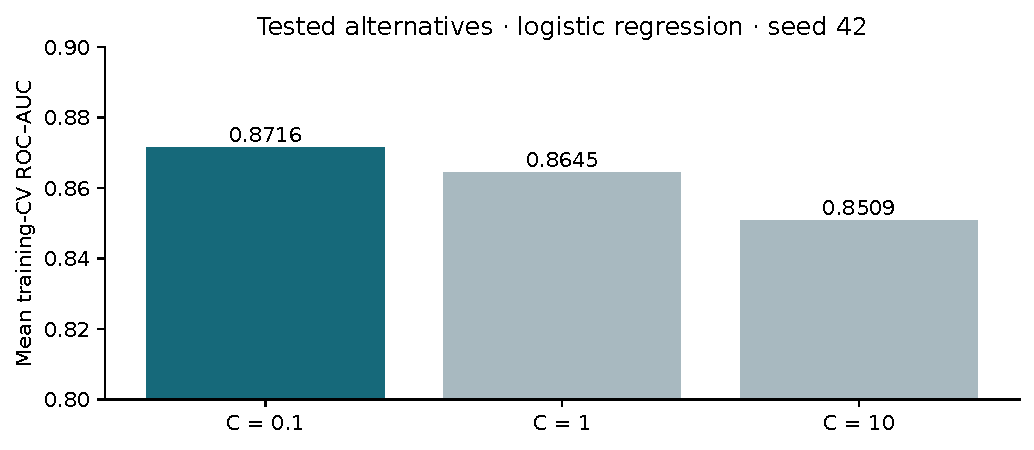
\includegraphics[width=0.88\textwidth]{figures/modeling/parameter_search.pdf}
\caption{Executed logistic-regression parameter alternatives for seed 42.
Scores are means over three training CV folds from the saved search output;
validation and test scores are not used in this parameter comparison.}
\label{fig:parameter-search}
\end{figure}


\section{Model Execution and Statistical Results}
\label{sec:model-building}
\subsection{Execution Protocol and Output Provenance}
\label{subsec:execution-protocol}
The construction and settings are specified in Sections~\ref{subsec:python-candidate-construction}
and~\ref{subsec:parameter-settings}. The evidence below is generated from
saved Python result files. It documents completed fits and held-out
predictions; it is not an SPSS interface capture or a new model run.
The holdout workflow compares five predictive families and a training-prior
dummy using both CART and RFE--CART selectors across five seeds.
The tuning workflow searches four individual families; stacking remains fixed.

\subsection{Evidence of Executed Models}
\label{subsec:execution-evidence}
\begin{table}[H]
\centering\small
\caption{Execution inventory counted from saved metrics and prediction files. Counts include the dummy where present and repeated evaluations of the same source records.}
\begin{tabular}{llll}
\toprule
Workflow & Metric rows & Prediction rows & Model families \\
\midrule
Fixed holdout & 120 & 5,760 & 6 \\
Tuned holdout & 25 & 1,200 & 4 \\
Leave-one-out & 6 & 1,914 & 6 \\
\bottomrule
\end{tabular}
\end{table}

Sources: \path{results/holdout/}, \path{results/tuning/} and \path{results/lopo/}, each containing \path{metrics.csv} and \path{predictions.csv}. Prediction rows are evaluation appearances, not unique patients. Saved fitted pipelines are in \path{models/holdout/}, \path{models/tuned/} and \path{models/lopo/}.

\begin{figure}[H]
\centering
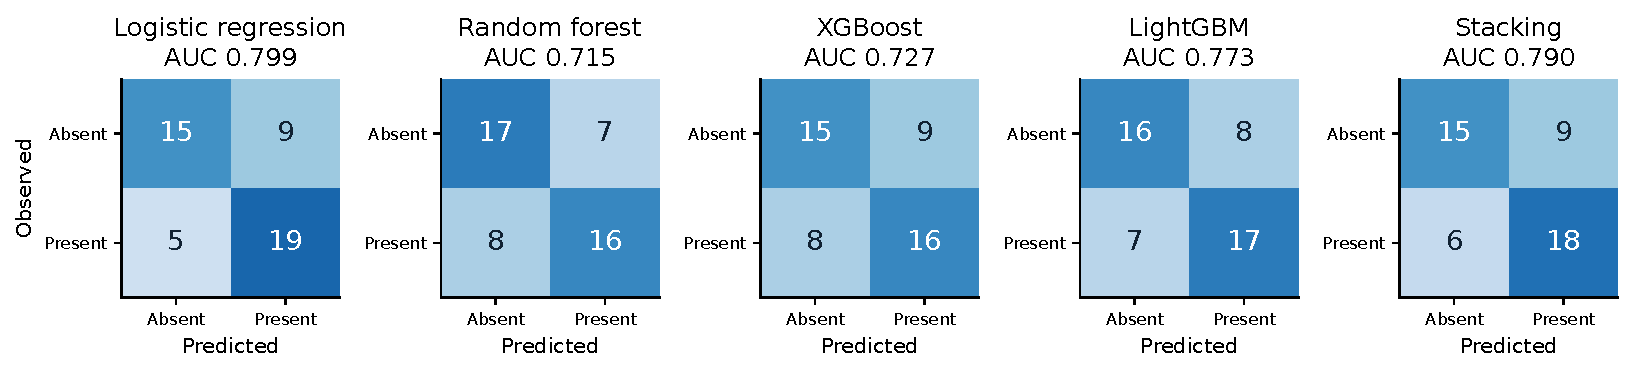
\includegraphics[width=\textwidth]{figures/modeling/execution_evidence.pdf}
\caption{Saved seed-42 validation outputs for all predictive families with
RFE--CART. Each confusion matrix contains 48 predictions at threshold 0.5;
class 1 denotes gallstones present. These are rendered numerical outputs,
not screenshots. Source: \protect\path{results/holdout/metrics.csv}.}
\label{fig:execution-evidence}
\end{figure}

\subsection{Statistical Patterns from the Fitted Models}
\label{subsec:statistical-patterns}
This section records numerical evidence. Interpretation is in
Section~\ref{subsec:pattern-discussion}, charts in
Section~\ref{subsec:pattern-visualisation}, and evaluation against the
project criteria in Section~\ref{subsec:model-evaluation}.

\paragraph{Holdout validation outputs.}
\label{subsec:python-building-selection}

Table~\ref{tab:building-validation-evidence} summarises the saved validation
results, not test rankings. Each cell reports mean $\pm$ sample variance
across five holdout seeds, using denominator $5-1$. This notation reports
variance, not standard deviation or a confidence interval. RFE denotes
RFE--CART; bold identifies the highest mean among predictive models in each
column, with the dummy shown separately as a benchmark.

\begin{table}[H]
\centering
\footnotesize
\setlength{\tabcolsep}{4pt}
\caption{Five-seed holdout validation: mean $\pm$ sample variance at threshold 0.5.}
\label{tab:building-validation-evidence}
\begin{tabular}{@{}lrrrr@{}}
\toprule
& \multicolumn{2}{c}{ROC--AUC} & \multicolumn{2}{c}{Sensitivity} \\
\cmidrule(lr){2-3}\cmidrule(l){4-5}
Model & CART & RFE & CART & RFE \\
\midrule
Logistic regression & $\mathbf{0.834 \pm 0.001306}$ & $\mathbf{0.838 \pm 0.001930}$ & $\mathbf{0.808 \pm 0.002257}$ & $\mathbf{0.758 \pm 0.002951}$ \\
Random forest       & $0.798 \pm 0.002135$ & $0.776 \pm 0.001504$ & $0.717 \pm 0.004688$ & $0.717 \pm 0.002083$ \\
XGBoost             & $0.791 \pm 0.001392$ & $0.777 \pm 0.001080$ & $0.742 \pm 0.003819$ & $0.708 \pm 0.000868$ \\
LightGBM            & $0.791 \pm 0.000612$ & $0.772 \pm 0.000973$ & $0.717 \pm 0.006424$ & $0.717 \pm 0.002083$ \\
Stacking            & $0.822 \pm 0.000825$ & $0.812 \pm 0.000558$ & $0.758 \pm 0.005556$ & $0.733 \pm 0.000521$ \\
\midrule
Training-prior dummy& $0.500 \pm 0.000000$ & $0.500 \pm 0.000000$ & $1.000 \pm 0.000000$ & $1.000 \pm 0.000000$ \\
\bottomrule
\end{tabular}
\end{table}

\paragraph{Leave-one-out outputs.}
\label{subsec:building-lopo-results}

Table~\ref{tab:building-lopo-results} reports the saved LOPO results from
\protect\path{results/lopo/metrics.csv}. Each model has 319 pooled held-out
predictions, using RFE--CART selection and seed 42. This is row-level LOOCV,
equivalent to leave-one-person-out only if each row is a different person.
There is one complete run, so no between-seed variance is reported. Bold marks
the highest predictive-model score in each column, except FNR, where lower
is better. These are complementary evaluation results, not a new basis for
overriding the validation-selected model family.

\begin{table}[H]
\centering
\small
\caption{LOPO evaluation on 319 held-out predictions per model at threshold 0.5.}
\label{tab:building-lopo-results}
\begin{tabular}{@{}lrrrrrr@{}}
\toprule
Model & Accuracy & ROC--AUC & Sensitivity & Specificity & F1 & FNR \\
\midrule
Logistic regression & 0.784 & \textbf{0.874} & 0.820 & 0.747 & 0.793 & 0.180 \\
Random forest & \textbf{0.799} & 0.857 & \textbf{0.839} & 0.759 & \textbf{0.808} & \textbf{0.161} \\
XGBoost & 0.762 & 0.835 & 0.807 & 0.715 & 0.774 & 0.193 \\
LightGBM & 0.787 & 0.851 & 0.832 & 0.741 & 0.798 & 0.168 \\
Stacking & 0.787 & 0.865 & 0.801 & \textbf{0.772} & 0.791 & 0.199 \\
\midrule
Training-prior dummy & 0.505 & 0.000 & 1.000 & 0.000 & 0.671 & 0.000 \\
\bottomrule
\end{tabular}
\end{table}


\paragraph{Numerical comparison of holdout and LOPO.}
The comparison fixes the algorithm settings and RFE--CART selector, avoiding
confounding evaluation method with CART versus RFE selection. Holdout test
entries describe every fixed candidate for comparison; they are not the
validation-selected procedure reported in Section~\ref{subsec:model-evaluation}.
Sources are \path{results/holdout/metrics.csv} and
\path{results/lopo/metrics.csv}. Interpretation and differences between the
evaluation designs are discussed in Section~\ref{par:holdout-lopo-discussion}.
\begin{table}[H]
\centering\small
\caption{Holdout and LOPO comparison for fixed RFE--CART candidates at threshold 0.5. Holdout entries average five seeds; LOPO entries pool 319 held-out predictions from one complete run.}
\label{tab:holdout-lopo-comparison}
\begin{tabular}{@{}lrrrrrr@{}}
\toprule
& \multicolumn{3}{c}{ROC--AUC} & \multicolumn{3}{c}{Sensitivity} \\
\cmidrule(lr){2-4}\cmidrule(l){5-7}
Model & Holdout val. & Holdout test & LOPO & Holdout val. & Holdout test & LOPO \\
\midrule
Logistic regression & 0.838 & 0.887 & 0.874 & 0.758 & 0.858 & 0.820 \\
Random forest & 0.776 & 0.850 & 0.857 & 0.717 & 0.850 & 0.839 \\
XGBoost & 0.777 & 0.844 & 0.835 & 0.708 & 0.858 & 0.807 \\
LightGBM & 0.772 & 0.841 & 0.851 & 0.717 & 0.850 & 0.832 \\
Stacking & 0.812 & 0.881 & 0.865 & 0.733 & 0.858 & 0.801 \\
\bottomrule
\end{tabular}
\end{table}


\paragraph{Conditional associations and extracted rules.}
Across five 20-feature RFE logistic fits, CRP, vitamin D, ECF/TBW and
haemoglobin were always selected, with mean transformed-scale coefficients
$-1.318$, $+0.690$, $+0.810$ and $+0.549$, respectively. Their mean validation
permutation AUC decreases were 0.1127, 0.0437, 0.0597 and 0.0172.
CRP was the root of all five direct CART selection trees: its recorded-scale
cut-point was 0.79 for seed 42 and 0.585 for the other four seeds.
The following counts describe seed-42 training nodes, not held-out risks.
\begin{table}[htbp]
\centering
\small
\caption{Conditional profiles extracted from the seed-42 CART selection tree.}
\label{tab:clinical-tree-patterns}
\begin{tabularx}{\textwidth}{Xrr}
\toprule
Model-defined subgroup & Present / total & Present (\%) \\
\midrule
CRP $\leq0.79$ & 100/138 & 72.5 \\
CRP $>0.79$ & 13/85 & 15.3 \\
CRP $\leq0.79$, total-body-fat ratio $\leq32.1$ & 87/107 & 81.3 \\
CRP $\leq0.79$, total-body-fat ratio $>32.1$ & 13/31 & 41.9 \\
CRP $>0.79$, vitamin D $\leq22.5$ & 3/60 & 5.0 \\
CRP $>0.79$, vitamin D $>22.5$ & 10/25 & 40.0 \\
\bottomrule
\end{tabularx}
\end{table}

\section{Interpretation, Evaluation and CRISP-DM Iteration}
\label{sec:multiple-iteration}
\subsection{Discussion of the Statistical Patterns}
\label{subsec:pattern-discussion}
Logistic regression has the strongest mean validation AUC under both
selectors. CART selection gives it higher sensitivity and F1 (0.761 versus
0.749 for RFE), despite slightly lower AUC. Stacking has lower between-seed
AUC variances (0.000825 with CART and 0.000558 with RFE) than logistic
regression (0.001306 and 0.001930), but also lower discrimination and sensitivity.
Thus, stability alone does not justify the added complexity. The dummy's
perfect sensitivity accompanies zero specificity and accuracy 0.500,
demonstrating why sensitivity cannot be the only criterion.

The implemented ranking uses descending validation AUC, descending accuracy,
and ascending FNR, followed by deterministic name-based tie-breaks. F1,
stability, and interpretability inform the discussion but are not numerical
components of this ranking. Logistic regression wins all five fixed-model
comparisons: CART is selected for seeds 42, 21, and 123, and RFE for seeds
7 and 84. This supports the simpler model family, not a universally best
selector or a claim of statistically significant superiority.

Tuning also selects logistic regression in all five seeds. The selected
$C$ values are 0.1, 0.1, 0.1, 1, and 10 in the stated seed order.
These choices come from training CV and validation, not test performance.
Selection does not guarantee the success criteria: for example, the seed-7
fixed-model winner has validation sensitivity 0.708. Recall is not a hard
eligibility constraint, and threshold optimisation and dedicated calibration
assessment remain unimplemented.

\subsubsection{Interpretation of the Leave-One-Out Results}
\label{subsec:lopo-interpretation}
The LOPO results in Table~\ref{tab:building-lopo-results} show a trade-off
between ranking patients by predicted probability and classifying them at
threshold 0.5. Logistic regression has the highest ROC--AUC (0.874), so it
provides the strongest overall discrimination among the tested models.
Its sensitivity of 0.820 corresponds to identifying 132 of 161 gallstone
records and missing 29; specificity of 0.747 corresponds to correctly
classifying 118 of 158 negative records, with 40 false positives. Thus,
meeting both 0.80 project benchmarks still leaves approximately 18\% of
positive records undetected. AUC alone does not establish calibration or
an acceptable operating threshold.

Random forest performs best at the fixed threshold: accuracy is 0.799,
sensitivity 0.839 and F1 0.808. It detects 135 positive records, misses 26
and produces 38 false positives. Compared with logistic regression, these
aggregate counts represent three fewer missed cases and two fewer false
alarms, despite a lower AUC of 0.857. This makes random forest a useful
candidate for further sensitivity-oriented validation, but the small observed
differences do not establish statistically significant superiority or justify
replacing the validation-selected family after inspecting LOPO results.

Stacking achieves the highest specificity (0.772), with 36 false positives,
but misses 32 positive records: its sensitivity of 0.801 only narrowly meets
the benchmark. Its extra complexity therefore does not deliver the best
case detection. LightGBM offers sensitivity 0.832 with 27 false negatives
and 41 false positives, while XGBoost has the lowest AUC (0.835) and
accuracy (0.762), with 31 false negatives and 45 false positives. All five
predictive models meet the two numerical benchmarks in this pooled run,
but their error trade-offs differ. The dummy's sensitivity of 1.000 is
uninformative without specificity: it incorrectly flags all 158 negative
records. Its unusual pooled AUC is explained below.

\subsubsection{Comparison of Holdout and Leave-One-Out Evaluation}
\label{par:holdout-lopo-discussion}
\begin{table}[H]
\centering\small
\caption{Roles and limitations of the two implemented evaluation methods.}
\label{tab:evaluation-method-comparison}
\begin{tabularx}{\textwidth}{@{}p{2.5cm}XX@{}}
\toprule
Dimension & Repeated stratified holdout & Leave-one-out (LOPO) \\
\midrule
Training and assessment &
223 training, 48 validation and 48 test records per seed. Selected
configurations and test-stage candidate fits use the 271 development records. &
318 training records and one held-out record per fold; 319 folds cover the
whole dataset once for each fixed candidate. \\
Role in this project &
Validation selects the model/selector; training CV selects tuning parameters.
Test results assess fitted candidates or the selected procedure. &
Provides complementary internal assessment of fixed RFE--CART candidates;
it does not repeat the entire model-selection process inside each fold. \\
Coverage and variation &
Five seeds expose split-to-split variation. Validation/test sets contain 48
records each, and records can recur across overlapping splits. &
Each source row contributes one held-out prediction per model. There is one
complete run; heavily overlapping training folds are not independent repeats. \\
Computation &
Fewer outer fits per fixed candidate; tuning and stacking add inner fits. &
319 outer fits per candidate, with additional inner fitting for stacking. \\
Interpretation boundary &
Performance depends on split composition and development size; inspected test
partitions are not a sealed external assessment. &
Uses more training data per prediction, but offers no external validation
and no between-seed variance estimate from the single run. \\
\bottomrule
\end{tabularx}
\end{table}

Table~\ref{tab:holdout-lopo-comparison} compares the same fixed RFE--CART
candidates. Logistic regression's AUC is 0.838 on holdout validation and
0.874 under LOPO, while sensitivity rises from 0.758 to 0.820. Across all
five families, LOPO AUC exceeds mean holdout-validation AUC by approximately
0.036--0.081, and sensitivity by 0.062--0.122. The pattern is consistent
with differences in training size (318 versus 223 records) and assessment
coverage, but this comparison cannot isolate their effects. It is not
evidence that changing the evaluation method improved an otherwise identical
fitted model.

The holdout \emph{test} comparison gives a different picture. Fixed RFE
logistic regression averages AUC 0.887 and sensitivity 0.858 on test,
compared with LOPO's 0.874 and 0.820. LOPO AUC is higher than mean holdout
test AUC for random forest and LightGBM, but lower for logistic regression,
XGBoost and stacking. LOPO sensitivity is lower for all five families.
Consequently, LOPO is not uniformly more favourable. Test fits use 271
development records and assess different, overlapping 48-row subsets;
LOPO evaluates every row with a separate 318-row training set. These
estimates answer related but different questions and should not be ranked
as if they were a controlled model-improvement experiment.

The two methods nevertheless agree that logistic regression has the highest
AUC among fixed RFE candidates. Their threshold-dependent rankings differ:
random forest leads LOPO sensitivity and F1, whereas logistic regression,
XGBoost and stacking share the highest mean RFE holdout-test sensitivity
when rounded to three decimals. This supports keeping discrimination,
sensitivity and false alarms separate in the decision. Use holdout validation
for the stated selection procedure and LOPO as a complementary robustness
check; neither establishes performance on a new cohort. LOPO is
leave-one-person-out only if each source row represents a unique person.
The single run supplies no evidence that LOPO has lower uncertainty than
repeated holdout, and its folds must not be treated as 319 independent
experiments.

\paragraph{Patterns across model families.}
\label{subsec:building-model-patterns}

The tables in Section~\ref{subsec:statistical-patterns} document the outputs for every fixed model. Their
patterns, rather than only the leading score, are summarised in
Table~\ref{tab:building-model-patterns}. Differences between holdout validation
and LOPO reflect different training sizes and evaluation samples; they do not
by themselves establish a statistically significant improvement.

\begin{table}[H]
\centering
\small
\caption{Observed performance patterns for every fixed model and benchmark.}
\label{tab:building-model-patterns}
\begin{tabularx}{\textwidth}{@{}p{2.8cm}X@{}}
\toprule
Model & Pattern and interpretation \\
\midrule
Logistic regression &
Leads validation AUC with either selector and retains the highest LOPO AUC.
CART improves validation sensitivity and F1 relative to RFE. Strong ranking
performance does not eliminate missed cases at threshold 0.5. \\
Random forest &
CART improves validation AUC over RFE without changing mean sensitivity.
Under LOPO it has the highest accuracy, sensitivity, and F1, and lowest FNR
among predictive models, but lower AUC than logistic regression. Its advantage
is threshold-specific case detection rather than the strongest ranking. \\
XGBoost &
CART improves validation AUC and sensitivity over RFE. It has the lowest
LOPO accuracy and AUC among predictive models, so the tested boosting
configuration provides no consistent advantage over simpler alternatives. \\
LightGBM &
CART improves validation AUC while mean sensitivity is unchanged. LOPO
sensitivity exceeds logistic regression's, but AUC and specificity are lower.
It offers a different error balance rather than dominance across metrics. \\
Stacking &
Validation AUC varies less across seeds than logistic regression's but has
a lower mean. LOPO gives the highest specificity and the highest FNR among
predictive models: fewer false alarms accompany more missed positive cases.
Combining models does not automatically improve all outcomes. \\
Training-prior dummy &
Predicts every evaluated row as positive at threshold 0.5. Perfect sensitivity
and zero FNR therefore accompany zero specificity and near-half accuracy;
this is a benchmark failure pattern, not useful disease discrimination. \\
\bottomrule
\end{tabularx}
\end{table}

The tuning experiment also built all four individual model families, not only
the selected logistic models. Their mean validation AUCs were 0.827 for
logistic regression, 0.779 for random forest, 0.777 for XGBoost, and 0.767
for LightGBM, from \protect\path{results/tuning/metrics.csv}. Relative to the fixed
RFE comparison, tuning did not consistently improve external-to-search
validation AUC: logistic regression and LightGBM decreased, random forest
increased slightly, and XGBoost was essentially unchanged at three decimal
places. Training-CV optimisation therefore does not guarantee validation
improvement. Stacking and the dummy were not tuned.

The dummy's pooled LOPO AUC is zero because leaving
out a positive case lowers the training prior while leaving out a negative
raises it, reversing the ranking of the fold-specific probabilities. A fixed
chance score instead has AUC 0.5.

\paragraph{Interpretation of fitted-model associations.}
\label{subsec:model-clinical-patterns}

The following evidence comes from fitted training models and validation perturbations, rather than repeated univariate EDA. Continuous logistic coefficients refer to one training-standard-deviation increase \emph{after} Yeo--Johnson transformation. They describe conditional model associations, not causal effects or original-unit clinical changes. CART rules come from the feature-selection tree, not a surrogate explanation of every ensemble.

\paragraph{Recurring signals and their direction.}
Four predictors recurred in all five 20-feature RFE fits: CRP, vitamin D, the ratio of extracellular fluid to total body water (\texttt{ecf\_tbw}), and haemoglobin. Their mean logistic coefficients were respectively $-1.318$, $+0.690$, $+0.810$ and $+0.549$, with the same sign in every split. CRP ranged from $-1.513$ to $-1.154$ and vitamin D from $+0.569$ to $+0.801$. Thus the fitted models combine laboratory and body-composition information rather than demographic risk alone.

Each raw predictor was also independently shuffled 20 times on each validation partition. Mean AUC decreases across five fits were 0.1127 for CRP, 0.0597 for \texttt{ecf\_tbw}, 0.0437 for vitamin D and 0.0172 for haemoglobin. These quantify perturbation-based contributions, not additive percentages of explained disease risk. The prominence of CRP, vitamin D and bioimpedance measurements agrees with the feature families reported by \textcite{esen2024early}; that study concerns the originating dataset and is not independent replication.

\paragraph{Thresholds and conditional interactions.}
CRP was the root split in all five direct CART selection trees, but its threshold varied: 0.79 for seed 42 and 0.585 for the other four seeds. Table~\ref{tab:clinical-tree-patterns} traces the seed-42 tree before transformation, retaining the recorded dataset scale. Counts describe training nodes, not externally validated risks or calibrated probabilities.



Body-fat ratio separates records within the low-CRP branch, whereas vitamin D separates those within the high-CRP branch. Within the low-CRP, higher-body-fat branch, visceral-fat rating $\leq10.5$ identifies 3/18 positive records, compared with 10/13 above 10.5. This suggests a candidate interaction between overall and visceral adiposity, not an established biological interaction. Different body-composition measures may capture different patient profiles, but these small, adaptively chosen groups require independent confirmation.

Crucially, lower CRP and higher vitamin D correspond to higher predicted gallstone presence here. These directions must not be rewritten as conventional causal risk statements. The outcome is existing gallstones; sampling, treatment or measurement context could affect associations. Learned cut-points are not clinical reference limits. Units and clinical context must be verified before treating any value as a diagnostic threshold; neither increasing CRP nor reducing vitamin D is a supported intervention.

\paragraph{Subgroup differences beyond a global coefficient.}
The female-versus-male logistic contrast was positive in all five models: the mean difference between their one-hot coefficients was $+0.814$, an odds multiplier of approximately 2.26 for that mean contrast, conditional on other transformed predictors. Nevertheless, seed 42's validation model missed 4 of 14 positive female records and 1 of 10 positive male records (27 female and 21 male records overall). A positive demographic coefficient therefore does not ensure equal identification: other covariates can outweigh it. Small denominators support a targeted audit, not a population-level fairness conclusion.

Hepatic-fat grades did not form a monotonic model pattern. Relative to grade 0, mean logistic contrasts were approximately $+0.819$ for grade 1, $-0.535$ for grade 2 and $-0.460$ for grade 3. These models therefore do not establish that increasing hepatic-fat severity increases gallstone risk. Conditional associations, sparse categories and overlapping metabolic measurements are competing explanations requiring clinical review.

\paragraph{Why weaker predictors contribute less.}
Selection alone does not establish useful prediction. Alkaline phosphatase was retained in all five RFE fits, yet its mean coefficient was only $-0.081$, changed sign across fits, and its mean validation permutation contribution was $-0.0024$. Triglycerides appeared in three fits, had mean coefficient $+0.013$ when selected, and mean perturbation contribution $-0.0055$ across all five fits. Negative contributions mean shuffling slightly improved validation discrimination, consistent with unstable or unnecessary fitted information; they do not indicate a protective clinical effect.

An excluded variable necessarily has zero permutation contribution in that pipeline. Age was excluded in every reference fit: this demonstrates non-use by the selector, not clinical irrelevance. Correlated measurements may substitute for each other, and single-variable permutation can understate shared information. RFE also ranks usefulness to CART, which need not match usefulness to the downstream logistic model.

The strongest signal is concentrated in CRP, but complementary contributions remain in fluid balance, vitamin D and smaller laboratory or categorical effects. The later 10-feature comparison in Section~\ref{subsec:iterations} tests retention of information in aggregate; it does not prove that every retained variable is necessary or identify which removed variable caused the loss. Grouped ablation would be needed to distinguish shared body-composition information from unique contributions.

\subsection{Visualisation of Model Patterns}
\label{subsec:pattern-visualisation}
\begin{figure}[H]
\centering
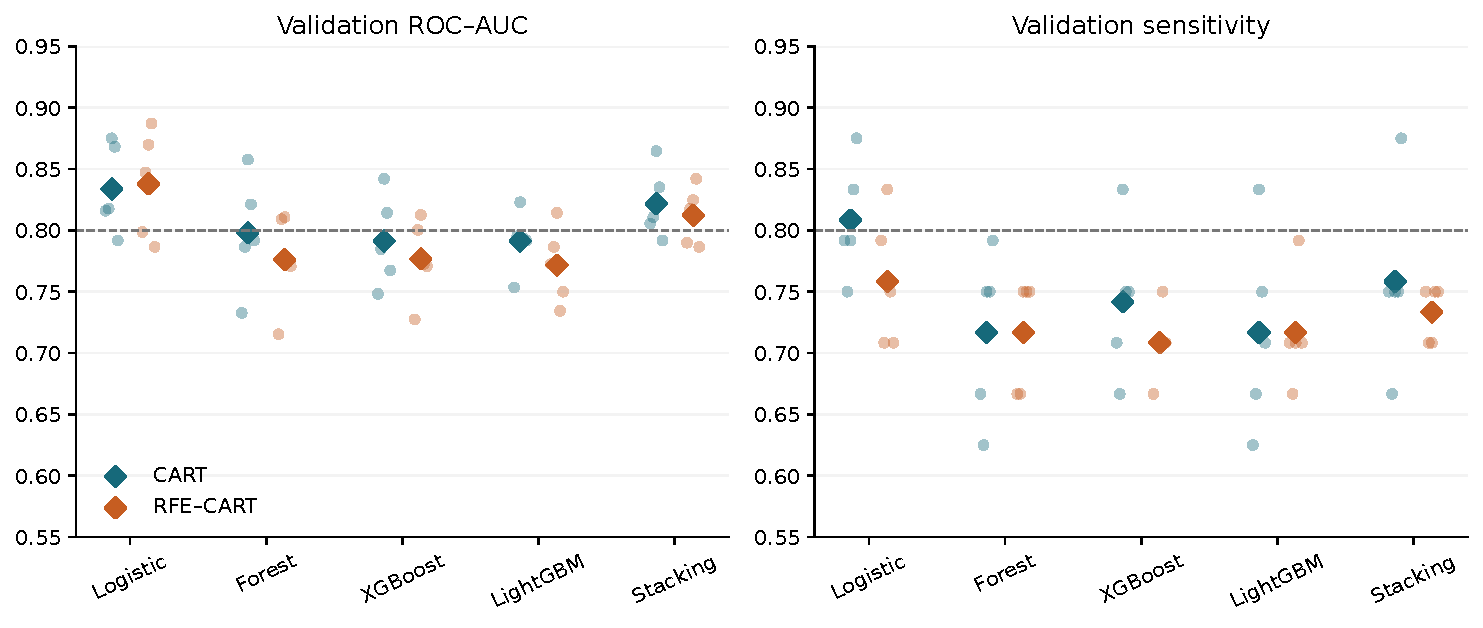
\includegraphics[width=\textwidth]{figures/modeling/model_comparison.pdf}
\caption{Validation discrimination and sensitivity for every predictive family
and selector. Large markers show five-seed means; small markers show individual
seeds, not confidence intervals. Dashed lines indicate the project benchmarks.
Source: \protect\path{results/holdout/metrics.csv}.}
\label{fig:model-comparison}
\end{figure}
\begin{figure}[H]
\centering
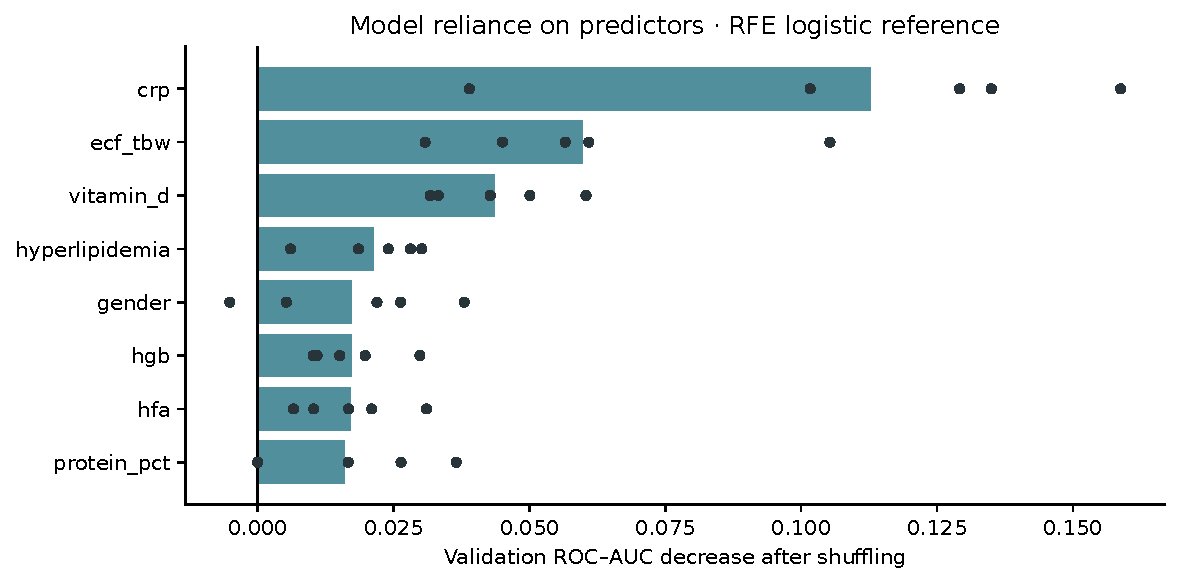
\includegraphics[width=0.93\textwidth]{figures/modeling/permutation_patterns.pdf}
\caption{Largest mean validation permutation contributions in the 20-feature
RFE logistic reference. Bars are mean AUC decreases; points are five fitted
splits, each averaging 20 shuffles. Correlated fields can share information;
these values are neither causal effects nor additive risk percentages.
Source: \protect\path{results/iteration_patterns/permutation.csv}.}
\label{fig:permutation-patterns}
\end{figure}
\subsection{Error Analysis: Repeatedly Misclassified Records}
\label{subsec:building-repeated-errors}

The saved prediction files permit review of errors that recur across seeds
and model families. Table~\ref{tab:building-repeated-errors} uses the
\emph{validation-selected fixed model} for each holdout seed, identified by
\protect\path{results/holdout/validation_winners.csv}, and its test predictions in
\protect\path{results/holdout/predictions.csv}. All these selected models are logistic
regression. Probabilities refer to gallstones being present; predictions use
threshold 0.5. The examples were chosen retrospectively to illustrate errors,
not to estimate their prevalence in future patients.

\begin{table}[H]
\centering
\small
\caption{Examples of repeated held-out errors; denominators count eligible test appearances.}
\label{tab:building-repeated-errors}
\begin{tabular}{@{}rlcrrr@{}}
\toprule
Source row & Holdout seeds & Error & Errors/runs & Probability range & LOPO errors/models \\
\midrule
117 & 7, 42      & FN & 2/2 & 0.068--0.350 & 4/5 \\
291 & 21, 42, 84 & FP & 3/3 & 0.703--0.758 & 5/5 \\
316 & 7, 84, 123 & FP & 3/3 & 0.634--0.794 & 5/5 \\
\bottomrule
\end{tabular}
\end{table}

\textbf{Record 117} has gallstones but was predicted absent in both holdout
test appearances. In LOPO, logistic regression, random forest, XGBoost, and
stacking also missed it; LightGBM correctly classified it with probability
0.566. The tuned holdout winners still missed it in both seeds. This is a
recurring false-negative example, although the LightGBM result shows that
the error is not universal across models.

\textbf{Records 291 and 316} have no gallstones but were repeatedly predicted
positive. Across all five predictive families and both selectors, record 291
was wrong in 29/30 holdout predictions and record 316 in 30/30; both were
false positives for all five LOPO models. Tuning corrected record 291 only
in seed 42, with probability 0.491, just below the decision threshold,
whereas record 316 remained wrong in all three tuned test appearances.
The first correction is therefore a borderline classification change, not
evidence that tuning consistently resolves the record's errors.

These identifiers are zero-based \texttt{source\_row} values, not verified
patient IDs. Repetition means the same dataset record was tested in several
overlapping splits or by different models, not that a patient had repeated
clinical visits. The LOPO denominator excludes the dummy benchmark. Shared
errors across model families motivate review of source measurements, labels,
and overlapping predictor profiles, but do not prove mislabelling or a causal
explanation. Their review must not be used to retune models and then claim
independent performance on the same test records.

\subsection{Model Evaluation Against the Project Objectives}
\label{subsec:model-evaluation}
\begin{table}[H]
\centering\small
\caption{Internal test performance of the validation-selected fixed procedure across five seeds. Ranges describe split variation, not confidence intervals.}
\begin{tabular}{lll}
\toprule
Metric & Mean & Minimum--maximum \\
\midrule
ROC--AUC & 0.883 & 0.828--0.915 \\
Sensitivity & 0.892 & 0.792--0.958 \\
Specificity & 0.708 & 0.667--0.792 \\
F1 & 0.816 & 0.769--0.846 \\
\bottomrule
\end{tabular}
\end{table}

These results come from \path{results/holdout/selected_test_metrics.csv}; selectors vary by seed. They describe the selected procedure, whereas the all-candidate tables in Section~\ref{subsec:statistical-patterns} describe individual models. Reused, overlapping test partitions limit independence.

The selected family is logistic regression, chosen using validation rather
than test ranking. Mean scores can meet a benchmark while individual splits
fail it. At the fixed 0.5 threshold, the RFE logistic reference has mean
validation AUC 0.838 but sensitivity 0.758: discrimination meets 0.80,
whereas case detection does not. The CART logistic candidate has means
0.834 and 0.808, but this does not establish reliable performance for every
split. LOPO logistic AUC 0.874 and sensitivity 0.820 are complementary
internal results for a fixed candidate, not a nested evaluation of selection.
The 20-feature RFE reference is consequently used for a controlled follow-up
experiment in Section~\ref{subsec:iterations}; it is not claimed to be the
selected selector in every seed.

\paragraph{Final fitting and evaluation integrity.}
\label{subsec:model-selection-feedback}

Selected configurations are refitted on the 271 development rows before
assessment on the 48 test rows. Complete pickle pipelines preserve preparation
and classifier state in \protect\path{models/holdout/} and \protect\path{models/tuned/}.
LOOCV evaluates fixed candidate pipelines by holding out each row once;
\protect\path{models/lopo/} contains separate full-data refits for future inference.
It is row-level evaluation, and it is not nested evaluation of the entire
algorithm-selection procedure.

The Iteration 2 concern is \textbf{partly resolved}: automatic selection now
excludes test scores, and the model-building argument above uses validation
evidence. However, the fixed-model notebook still evaluates every candidate
on test before recording its validation winner, and tuning reuses those
partitions. The resulting exposure permits informal test-driven decisions.
Overlapping splits and prior dataset exploration further limit independence;
the results must be described as internal evaluations.

A stricter future workflow would lock the complete configuration before
accessing an untouched test set and evaluate only that configuration.
Alternatively, nested outer evaluation should contain all selection decisions
within its training folds. Error analysis may motivate later revisions, but
revised models require new assessment. This qualification addresses the
feedback without claiming that the current implementation provides a fully
sealed final test.

\paragraph{Decision and feedback trigger.}
Retain logistic regression as the leading research family, but do not claim
that the current workflow establishes deployment readiness. Calibration,
threshold selection, generalisation and the cost of false positives remain
unresolved. Variable sensitivity and recurring errors motivate returning to
feature selection after this evaluation. The next subsection records the
completed controlled revision, including its unsuccessful outcome.
\subsection{A Completed CRISP-DM Feedback Cycle}
\label{subsec:iterations}

The Python/Jupyter workflow follows CRISP-DM as a feedback cycle. The business objective remains to support assessment of gallstone presence, with missed cases a particular concern; this is not a prospective disease-onset model. Sections~\ref{sec:model-building} and~\ref{subsec:model-evaluation} report execution evidence and the model evaluation. Here, evaluation motivates a return to feature selection, followed by an executed rerun and a documented decision.

\paragraph{Cycle A: establish and evaluate the reference.}
Data understanding established the coded categories and outcome direction: source status 0 becomes modelling class 1 (gallstones present). Data preparation fitted imputation, CART-based recursive feature elimination (RFE; 20 predictors), Yeo--Johnson transformation and standardisation on each training partition. Logistic regression used $C=1$ and a 0.5 classification threshold. Five stratified 70--15--15 splits used seeds 42, 7, 21, 84 and 123, with 223 training, 48 validation and 48 test records each. Evaluation exposed variable sensitivity and recurring errors, prompting the question: does a smaller predictor set remove unstable information without losing useful signal?

\paragraph{Cycle B: revisit preparation, rebuild and re-evaluate.}
A focused revision reduced RFE from 20 to 10 predictors. This was the only changed modelling choice: rows, seeds, transformations, logistic settings and threshold remained fixed. All preprocessing and feature selection were fitted again on the 223 training records, and both cycles were rerun on the corresponding validation records. No test records were evaluated in this additional experiment. This completes the loop
\emph{evaluation $\rightarrow$ revised data preparation $\rightarrow$ modelling $\rightarrow$ evaluation $\rightarrow$ decision}, rather than merely proposing future work.

\begin{table}[htbp]
\centering
\small
\caption{Paired validation comparison. Summary entries are mean $\pm$ sample variance across five seeds, not standard deviation. Bold indicates the higher mean or seed-level value.}
\label{tab:iteration-summary}
\begin{tabular}{lrrrr}
\toprule
& \multicolumn{2}{c}{Validation AUC} & \multicolumn{2}{c}{Sensitivity} \\
Seed & 20 features & 10 features & 20 features & 10 features \\
\midrule
42  & \textbf{0.799} & 0.760 & \textbf{0.792} & \textbf{0.792} \\
7   & \textbf{0.847} & 0.825 & \textbf{0.708} & 0.667 \\
21  & \textbf{0.870} & 0.826 & \textbf{0.833} & 0.750 \\
84  & \textbf{0.887} & 0.856 & \textbf{0.750} & \textbf{0.750} \\
123 & 0.786 & \textbf{0.811} & 0.708 & \textbf{0.792} \\
\midrule
Mean $\pm$ variance &
$\mathbf{0.838}\pm0.001930$ & $0.816\pm0.001223$ &
$\mathbf{0.758}\pm0.002951$ & $0.750\pm0.002604$ \\
\bottomrule
\end{tabular}
\end{table}


\begin{figure}[H]
\centering
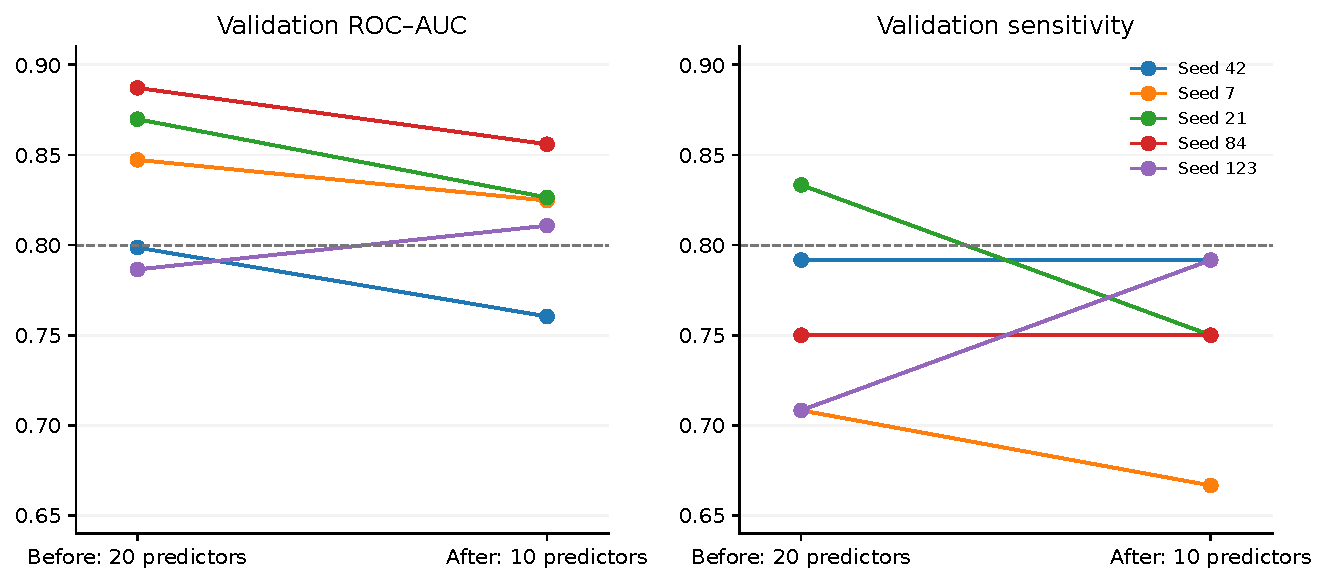
\includegraphics[width=\textwidth]{figures/modeling/iteration_comparison.pdf}
\caption{Completed feedback cycle: paired validation results before and after
reducing RFE from 20 to 10 predictors. Each line connects the same seed;
all other modelling choices are held fixed. Dashed lines mark the 0.80
project targets. Source: \protect\path{results/iteration_patterns/cycle_metrics.csv}.}
\label{fig:iteration-comparison}
\end{figure}

\paragraph{Decision and robustness boundary.}
The revision lowered AUC in four of five splits, with a mean change of $-0.0222$; sensitivity fell by 0.0083 on average. Lower between-seed variance did not compensate for lower discrimination or resolve missed cases. The 20-feature reference was therefore retained for this comparison. This tests robustness to a specific simplification, not universal superiority: validation partitions overlap across seeds, have already informed development, and neither cycle achieved mean sensitivity of 0.80. The revised model was not promoted to the saved candidate folders. Separate tuning and LOPO results remain in Sections~\ref{subsec:parameter-settings} and~\ref{subsec:statistical-patterns}; they are not independent external confirmation of this iteration.

\paragraph{Proposed next feedback cycle.}
The completed comparison shows that reducing the number of predictors alone
does not resolve missed cases. Table~\ref{tab:next-dm-cycle} translates this
finding and the remaining evaluation gaps into specific preparation and
modelling changes. These are proposed experiments, not additional completed
cycles. Each experiment should record its motivating finding, controlled
change, evaluation result and retain-or-reject decision.

\begin{table}[htbp]
\centering
\small
\caption{Proposed changes for the next CRISP-DM feedback cycle.}
\label{tab:next-dm-cycle}
\begin{tabularx}{\textwidth}{@{}p{2.3cm}XX@{}}
\toprule
Area & Proposed change and rationale & Evaluation and decision rule \\
\midrule
Feature engineering &
Test a small, prespecified set of representations or interactions, such as
overall-by-visceral adiposity, motivated by conditional model patterns.
Verify units and measurement availability; distinguish existing ratios from
newly engineered features. &
Compare against the unchanged logistic reference using paired development
folds. Fit transformations within training folds and retain changes only
when validation supports their contribution. \\
\addlinespace
Feature importance &
Use grouped permutation and refitted group ablation for correlated fluid,
adiposity and laboratory measurements, extending individual importance
estimates. &
Compare AUC, sensitivity and stability. Distinguish a fitted model's reliance
on a variable group from the performance achievable after refitting without
it; low individual importance alone does not justify removal. \\
\addlinespace
Feature selection &
Compare the 20-feature RFE reference with logistic-compatible selection,
regularised logistic regression using all eligible predictors, and a
predefined routine-measurement subset. &
Choose feature counts and penalties within inner development folds. Assess
performance and measurement burden together; the unsuccessful 10-feature
revision does not establish that every retained field is necessary. \\
\addlinespace
Calibration and threshold &
Assess probability calibration and select a threshold using a prespecified
sensitivity target and an agreed specificity or assessment-workload
constraint. &
Fit any calibrator and choose the threshold within development data using
held-out predictions. Freeze both before outer evaluation; report
calibration, sensitivity, specificity and confusion counts. \\
\addlinespace
Subgroup evaluation &
Extend the preliminary sex-specific error review to predefined sex and age
groups, checking measurement quality and sample support. &
Report group sizes, positive counts, error rates and uncertainty. Small
groups support further investigation rather than firm fairness claims. \\
\bottomrule
\end{tabularx}
\end{table}

All feature, model, calibration and threshold choices must remain inside the
development process. Because the current test partitions have already been
inspected, subsequent results on those records remain exploratory. Nested
evaluation can assess a prespecified selection procedure internally, while an
untouched external cohort is needed to examine transfer beyond this dataset.
If no candidate satisfies the predefined success criteria, the next cycle
should report that outcome rather than select a model by AUC alone.

\subsection{Return to Business Understanding and Deployment}
\label{subsec:business-objective-evaluation}

The completed cycle supports a research screening aid, not deployment or replacement of clinical assessment. Simplification can sacrifice complementary information without resolving false negatives. Repeatedly misclassified records documented in Section~\ref{subsec:building-repeated-errors} should guide source-data and subgroup review, not retrospective relabelling. The next CRISP-DM cycle should specify calibration and sensitivity-oriented threshold selection within development data, then assess the frozen pipeline on an untouched external cohort. These steps are planned, not claimed as completed.

\paragraph{Reproducibility.}
The executed comparison and pattern extraction are implemented in
\protect\path{scripts/iteration_pattern_analysis.py}, using the existing \protect\path{utils.py}.
The folder \protect\path{results/iteration_patterns/} records per-seed cycle results,
sample variances, selected fields, coefficients, validation permutation
contributions, subgroup counts, CART node counts and the source-data signature.
The analysis refits training-specific transformations from raw records; it does
not evaluate the full-data reference transformed CSV.


% \section{Limitation and Challenges of SPSS Modeler Workflow}
% \label{subsec:spss-limitations}
% Although SPSS Modeler provides a structured visual environment that aligns well with many CRISP-DM activities, several practical limitations were encountered during this project. In particular, not every CRISP-DM phase can be represented directly as a modelling node. Activities such as business understanding, interpretation of clinical requirements, and deployment planning still require substantial documentation and reasoning outside the
SPSS stream.

Model refinement was also relatively manual. Although SPSS provides automated modelling facilities for comparing multiple algorithms, detailed hyperparameter tuning often requires individual model nodes to be configured,
executed, and compared repeatedly. This makes systematic tuning less flexible than programmatic frameworks where parameter searches, cross-validation, and experiment tracking can be automated more easily.

The range of algorithms and transformations available also depends on the
installed SPSS Modeler version and extensions. Some newer machine-learning methods and specialised preprocessing techniques are less readily available
than in Python or R ecosystems. Similarly, custom feature engineering and complex pipeline logic can become difficult to maintain when a stream contains
many connected nodes.

Another challenge concerns reproducibility and workflow management. The visual stream is useful for demonstrating the sequence of CRISP-DM activities, but changes to parameters and intermediate nodes must be carefully documented to
ensure that modelling iterations can be reproduced. For this reason, key settings, transformations, partitions, selected variables, and evaluation
results were explicitly recorded in the report.

Finally, deployment in this iteration is limited to demonstrating a model-ready SPSS workflow rather than implementing a production clinical
application. A real deployment would additionally require automated data ingestion, monitoring, model versioning, security controls, and integration with healthcare information systems.

Despite these limitations, SPSS Modeler was appropriate for this iteration because its visual workflow clearly demonstrates the relationship between data understanding, preparation, transformation, modelling, and evaluation.
The limitations mainly affect scalability, automation, and production deployment rather than the ability to conduct the current proof-of-concept
classification analysis.

% \appendix


\newpage
% Acknowledgement
\section{Acknoledgement}
I acknowledge that this submission is my own original work and has been prepared in accordance with the University of Auckland's policies on academic integrity and copyright. Further information is available from the
\href{https://www.auckland.ac.nz/en/students/forms-policies-and-guidelines/student-policies-and-guidelines/academic-integrity-copyright.html}
{University of Auckland Academic Integrity and Copyright guidelines}.

I also confirm that I have the appropriate permission to use the data included in this project. Where data are owned by an organisation and are not publicly available, permission must be obtained from the relevant rights holder, including permission to upload the data to Canvas. The University of Auckland accepts no responsibility for any misuse of data by the student.

\subsection*{Use of Artificial Intelligence}
Generative artificial intelligence tools were used to support language editing, sentence restructuring, LaTeX formatting, and the organisation of the report. All project decisions, data analysis, interpretation of results, and final content were reviewed and completed by the author. No confidential, personal, or restricted data were shared with an artificial intelligence tool.

% REFERENCES
\newpage

\printbibliography[
    heading=bibintoc,
    title={References}
]

\clearpage
\appendix
\section{Instructions for Running the Submitted Workflow}
\label{app:running-workflow}
This appendix explains how to run the submitted Iteration 3 Python/Jupyter
workflow. All commands below are run from the \path{Iteration3_OpenStack}
directory unless stated otherwise. Keep the supplied directory structure intact.

\subsection{Environment and Required Files}

Install Python and create a dedicated virtual environment. The submitted
notebooks record Python 3.13.5; package requirements are minimum versions rather
than an exact environment lock. On macOS or Linux, run:

\begin{verbatim}
cd INFOSYS722/Iteration3_OpenStack
python3 -m venv .venv
source .venv/bin/activate
python -m pip install -r requirements.txt
python -m ipykernel install --sys-prefix \
  --name gallstone-iteration3 \
  --display-name "Gallstone Iteration 3"
\end{verbatim}

On Windows PowerShell, create the environment with
\texttt{python -m venv .venv} and activate it using
\path{.venv\Scripts\Activate.ps1}. Run the kernel-install command on one line,
omitting the shell continuation backslashes.

The active modelling workflow requires \path{data/raw/dataset_gallstone},
which is a CSV file with no extension. Preserve its filename and row order.
The accompanying \path{data/raw/dataset_gallstone.xlsx} is also supplied, but
does not replace the extensionless CSV used by the modelling functions.
Keep \path{utils.py}, \path{modeling.py}, \path{requirements.txt},
\path{run_workflow.py}, and the \path{notebooks/}, \path{scripts/},
\path{tests/} and \path{Report/} directories together with the raw data.

\subsection{Run the Complete Workflow}

The runner executes the stages sequentially and stops if a stage fails:

\begin{verbatim}
python run_workflow.py --list
python run_workflow.py
\end{verbatim}

The first command only lists the stages; the second runs the complete analysis,
regenerates report figures and tables, and runs the workflow checks. Execution
overwrites notebook outputs, generated data, result files and saved models.
Use a separate copy of the submission to preserve the supplied results.
Each execution records Python and installed package versions in
\path{results/runs/}. Leave-one-out evaluation and stacking involve many model
fits and can take substantially longer than the other stages.

The execution order and main outputs are:

\begin{enumerate}[leftmargin=*]
  \item \textbf{Exploration (\texttt{eda}):}
  \path{notebooks/gallstone_eda.ipynb} explores the original data.
  \item \textbf{Preparation (\texttt{prepare}):}
  \path{notebooks/transformation_feature_engineering.ipynb} exports
  training-fitted transformations and partitions to \path{data/processed/}.
  \item \textbf{Holdout evaluation (\texttt{holdout}):}
  \path{notebooks/holdout_method.ipynb} writes metrics and predictions to
  \path{results/holdout/} and pipelines to \path{models/holdout/}.
  \item \textbf{Leave-one-out evaluation (\texttt{lopo}):}
  \path{notebooks/leave_one_out_method.ipynb} evaluates 319 held-out rows
  per model family and writes \path{results/lopo/} and \path{models/lopo/}.
  \item \textbf{Parameter tuning (\texttt{tuning}):}
  \path{notebooks/tuning_model.ipynb} writes search and evaluation results
  to \path{results/tuning/} and selected models to \path{models/tuned/}.
  \item \textbf{Error analysis (\texttt{errors}):}
  \path{notebooks/error_analysis.ipynb} reads saved predictions and writes
  \path{results/error_analysis/}.
  \item \textbf{Iteration comparison (\texttt{patterns}):}
  \path{scripts/iteration_pattern_analysis.py} compares the 20- and
  10-predictor references and writes \path{results/iteration_patterns/}.
  \item \textbf{Report outputs (\texttt{figures}):}
  \path{Report/build_modeling_figures.py} regenerates modelling figures
  and evidence tables in \path{Report/figures/modeling/} and
  \path{Report/generated/} from saved results.
  \item \textbf{Verification (\texttt{check}):} unit checks cover preparation
  isolation, saved-pipeline prediction consistency and disease-positive
  label/false-negative-rate coding.
\end{enumerate}

For interactive execution, run \texttt{python -m jupyter lab}, select the
\textbf{Gallstone Iteration 3} kernel and use \textbf{Restart Kernel and Run
All Cells} for each of the six notebooks in the order above. Complete each
notebook before opening the next stage, then run:

\begin{verbatim}
python scripts/iteration_pattern_analysis.py
python Report/build_modeling_figures.py
python -m unittest discover -s tests -v
\end{verbatim}

\subsection{Resume Execution and Check Results}

To restart at a failed stage, use \texttt{--from-stage}. To run just one stage,
also specify \texttt{--to-stage}, for example:

\begin{verbatim}
python run_workflow.py --from-stage tuning
python run_workflow.py --from-stage holdout --to-stage holdout
python run_workflow.py --from-stage check
\end{verbatim}

Stage selection does not rebuild prerequisites: tuning requires prepared data,
and complete error analysis requires the preceding evaluation results. After
changing data, seeds, preparation or model settings, rerun from
\texttt{prepare} through the end; rerun exploration when raw data change.
An interrupted stage is not a completed result.

Check \path{data/processed/manifest.json} and split-membership files for seeds
42, 7, 21, 84 and 123, with 223 training, 48 validation and 48 test rows per
seed. A complete fixed holdout run produces 120 metric rows and 5,760 prediction
rows; LOPO produces six metric rows and 1,914 predictions; tuning produces
25 metric rows and 1,200 predictions. These appear in the respective
\path{results/holdout/}, \path{results/lopo/} and \path{results/tuning/}
directories as \path{metrics.csv} and \path{predictions.csv}.
The checks verify selected workflow invariants rather than every reported score.

Fixed seeds support repeatability within an environment, but package and
platform differences can change exact results. Supplied pickle files require
compatible library versions; if incompatible, regenerate preparation and
models from \texttt{prepare} onward in the new environment. Evaluation must
use the training-fitted partitions, not a new random split of the full-data
\path{transformed_dataset.csv}.

\subsection{Rebuild the Report PDF}

With saved results present, regenerate the modelling figures and tables without
retraining using the first command below. Install a LaTeX distribution with
\texttt{latexmk}, \texttt{pdflatex}, Biber and the packages declared in
\path{Report/main.tex}, then compile:

\begin{verbatim}
python Report/build_modeling_figures.py
latexmk -pdf -interaction=nonstopmode -halt-on-error \
  -cd Report/main.tex
\end{verbatim}

On PowerShell, enter the \texttt{latexmk} command on one line without the
continuation backslash. The compiled report is \path{Report/main.pdf}.
Retain all report source files, \path{references.bib}, \path{media/}, figures
and generated tables. Figure generation does not update earlier exploratory
images or manually written tables and discussion; reconcile those passages
with any changed results before compiling the final report.


\end{document}
